\documentclass{article}


\usepackage{amssymb}
\usepackage{amsmath}
\usepackage{graphicx}
\usepackage{xspace}
\usepackage{cite}
\usepackage{color}
\usepackage{tabularx}
\usepackage{multirow}
\usepackage{booktabs}
\usepackage{array}
\usepackage{ragged2e}
\usepackage{url}
%\usepackage[table]{xcolor}
\usepackage{colortbl}
%\usepackage{supertabular}
\usepackage{longtable}
\usepackage{listings}
\usepackage[normalem]{ulem}
\usepackage{subcaption}
\usepackage{placeins}

\newcommand{\DefMacro}[2]{\expandafter\newcommand\csname rmk-#1\endcsname{#2}}
\newcommand{\UseMacro}[1]{\csname rmk-#1\endcsname}

\newcolumntype{R}[1]{>{\RaggedLeft\arraybackslash}p{#1}}
\newcolumntype{L}[1]{>{\RaggedRight\arraybackslash}p{#1}}

%%% Automatically generated by run_examples.py
\DefMacro{LANG883Id}{LANG-883}
\DefMacro{LANG883OrigHisLen}{262}
\DefMacro{LANG883OrigSliceSize}{44}
\DefMacro{LANG883OrigFuncCount}{5}
\DefMacro{LANG883OrigCompCount}{2}
\DefMacro{LANG883OrigHunkCount}{37}
\DefMacro{LANG883OrigASTLineCount}{478}
\DefMacro{LANG883SplitHisLen}{504}
\DefMacro{LANG883SplitSliceSize}{8}
\DefMacro{LANG883SplitFuncCount}{5}
\DefMacro{LANG883SplitCompCount}{2}
\DefMacro{LANG883SplitHunkCount}{1}
\DefMacro{LANG883SplitASTLineCount}{478}
\DefMacro{LANG883SplitSliceSizeMapBack}{8}
\DefMacro{LANG883Reduction}{81.82}
\DefMacro{LANG993Id}{LANG-993}
\DefMacro{LANG993OrigHisLen}{262}
\DefMacro{LANG993OrigSliceSize}{62}
\DefMacro{LANG993OrigFuncCount}{2}
\DefMacro{LANG993OrigCompCount}{2}
\DefMacro{LANG993OrigHunkCount}{58}
\DefMacro{LANG993OrigASTLineCount}{407}
\DefMacro{LANG993SplitHisLen}{504}
\DefMacro{LANG993SplitSliceSize}{4}
\DefMacro{LANG993SplitFuncCount}{2}
\DefMacro{LANG993SplitCompCount}{2}
\DefMacro{LANG993SplitHunkCount}{0}
\DefMacro{LANG993SplitASTLineCount}{407}
\DefMacro{LANG993SplitSliceSizeMapBack}{4}
\DefMacro{LANG993Reduction}{93.55}
\DefMacro{LANG1006Id}{LANG-1006}
\DefMacro{LANG1006OrigHisLen}{262}
\DefMacro{LANG1006OrigSliceSize}{51}
\DefMacro{LANG1006OrigFuncCount}{3}
\DefMacro{LANG1006OrigCompCount}{2}
\DefMacro{LANG1006OrigHunkCount}{46}
\DefMacro{LANG1006OrigASTLineCount}{489}
\DefMacro{LANG1006SplitHisLen}{504}
\DefMacro{LANG1006SplitSliceSize}{7}
\DefMacro{LANG1006SplitFuncCount}{3}
\DefMacro{LANG1006SplitCompCount}{2}
\DefMacro{LANG1006SplitHunkCount}{2}
\DefMacro{LANG1006SplitASTLineCount}{489}
\DefMacro{LANG1006SplitSliceSizeMapBack}{7}
\DefMacro{LANG1006Reduction}{86.27}
\DefMacro{LANG1080Id}{LANG-1080}
\DefMacro{LANG1080OrigHisLen}{262}
\DefMacro{LANG1080OrigSliceSize}{75}
\DefMacro{LANG1080OrigFuncCount}{7}
\DefMacro{LANG1080OrigCompCount}{0}
\DefMacro{LANG1080OrigHunkCount}{68}
\DefMacro{LANG1080OrigASTLineCount}{638}
\DefMacro{LANG1080SplitHisLen}{504}
\DefMacro{LANG1080SplitSliceSize}{7}
\DefMacro{LANG1080SplitFuncCount}{7}
\DefMacro{LANG1080SplitCompCount}{0}
\DefMacro{LANG1080SplitHunkCount}{0}
\DefMacro{LANG1080SplitASTLineCount}{638}
\DefMacro{LANG1080SplitSliceSizeMapBack}{7}
\DefMacro{LANG1080Reduction}{90.67}
\DefMacro{LANG1093Id}{LANG-1093}
\DefMacro{LANG1093OrigHisLen}{262}
\DefMacro{LANG1093OrigSliceSize}{65}
\DefMacro{LANG1093OrigFuncCount}{3}
\DefMacro{LANG1093OrigCompCount}{4}
\DefMacro{LANG1093OrigHunkCount}{58}
\DefMacro{LANG1093OrigASTLineCount}{446}
\DefMacro{LANG1093SplitHisLen}{504}
\DefMacro{LANG1093SplitSliceSize}{11}
\DefMacro{LANG1093SplitFuncCount}{3}
\DefMacro{LANG1093SplitCompCount}{4}
\DefMacro{LANG1093SplitHunkCount}{4}
\DefMacro{LANG1093SplitASTLineCount}{446}
\DefMacro{LANG1093SplitSliceSizeMapBack}{11}
\DefMacro{LANG1093Reduction}{83.08}
\DefMacro{IO173Id}{IO-173}
\DefMacro{IO173OrigHisLen}{136}
\DefMacro{IO173OrigSliceSize}{21}
\DefMacro{IO173OrigFuncCount}{7}
\DefMacro{IO173OrigCompCount}{0}
\DefMacro{IO173OrigHunkCount}{14}
\DefMacro{IO173OrigASTLineCount}{315}
\DefMacro{IO173SplitHisLen}{546}
\DefMacro{IO173SplitSliceSize}{9}
\DefMacro{IO173SplitFuncCount}{8}
\DefMacro{IO173SplitCompCount}{0}
\DefMacro{IO173SplitHunkCount}{1}
\DefMacro{IO173SplitASTLineCount}{315}
\DefMacro{IO173SplitSliceSizeMapBack}{8}
\DefMacro{IO173Reduction}{61.90}
\DefMacro{IO275Id}{IO-275}
\DefMacro{IO275OrigHisLen}{136}
\DefMacro{IO275OrigSliceSize}{46}
\DefMacro{IO275OrigFuncCount}{6}
\DefMacro{IO275OrigCompCount}{0}
\DefMacro{IO275OrigHunkCount}{40}
\DefMacro{IO275OrigASTLineCount}{333}
\DefMacro{IO275SplitHisLen}{546}
\DefMacro{IO275SplitSliceSize}{13}
\DefMacro{IO275SplitFuncCount}{7}
\DefMacro{IO275SplitCompCount}{0}
\DefMacro{IO275SplitHunkCount}{6}
\DefMacro{IO275SplitASTLineCount}{333}
\DefMacro{IO275SplitSliceSizeMapBack}{12}
\DefMacro{IO275Reduction}{73.91}
\DefMacro{IO288Id}{IO-288}
\DefMacro{IO288OrigHisLen}{136}
\DefMacro{IO288OrigSliceSize}{2}
\DefMacro{IO288OrigFuncCount}{2}
\DefMacro{IO288OrigCompCount}{0}
\DefMacro{IO288OrigHunkCount}{0}
\DefMacro{IO288OrigASTLineCount}{520}
\DefMacro{IO288SplitHisLen}{546}
\DefMacro{IO288SplitSliceSize}{1}
\DefMacro{IO288SplitFuncCount}{1}
\DefMacro{IO288SplitCompCount}{0}
\DefMacro{IO288SplitHunkCount}{0}
\DefMacro{IO288SplitASTLineCount}{260}
\DefMacro{IO288SplitSliceSizeMapBack}{1}
\DefMacro{IO288Reduction}{50.00}
\DefMacro{IO290Id}{IO-290}
\DefMacro{IO290OrigHisLen}{136}
\DefMacro{IO290OrigSliceSize}{47}
\DefMacro{IO290OrigFuncCount}{5}
\DefMacro{IO290OrigCompCount}{0}
\DefMacro{IO290OrigHunkCount}{42}
\DefMacro{IO290OrigASTLineCount}{278}
\DefMacro{IO290SplitHisLen}{546}
\DefMacro{IO290SplitSliceSize}{10}
\DefMacro{IO290SplitFuncCount}{5}
\DefMacro{IO290SplitCompCount}{0}
\DefMacro{IO290SplitHunkCount}{5}
\DefMacro{IO290SplitASTLineCount}{278}
\DefMacro{IO290SplitSliceSizeMapBack}{10}
\DefMacro{IO290Reduction}{78.72}
\DefMacro{IO305Id}{IO-305}
\DefMacro{IO305OrigHisLen}{136}
\DefMacro{IO305OrigSliceSize}{59}
\DefMacro{IO305OrigFuncCount}{8}
\DefMacro{IO305OrigCompCount}{0}
\DefMacro{IO305OrigHunkCount}{51}
\DefMacro{IO305OrigASTLineCount}{571}
\DefMacro{IO305SplitHisLen}{546}
\DefMacro{IO305SplitSliceSize}{15}
\DefMacro{IO305SplitFuncCount}{8}
\DefMacro{IO305SplitCompCount}{0}
\DefMacro{IO305SplitHunkCount}{7}
\DefMacro{IO305SplitASTLineCount}{571}
\DefMacro{IO305SplitSliceSizeMapBack}{15}
\DefMacro{IO305Reduction}{74.58}
\DefMacro{COMPRESS327Id}{COMPRESS-327}
\DefMacro{COMPRESS327OrigHisLen}{148}
\DefMacro{COMPRESS327OrigSliceSize}{68}
\DefMacro{COMPRESS327OrigFuncCount}{49}
\DefMacro{COMPRESS327OrigCompCount}{1}
\DefMacro{COMPRESS327OrigHunkCount}{18}
\DefMacro{COMPRESS327OrigASTLineCount}{7213}
\DefMacro{COMPRESS327SplitHisLen}{365}
\DefMacro{COMPRESS327SplitSliceSize}{122}
\DefMacro{COMPRESS327SplitFuncCount}{112}
\DefMacro{COMPRESS327SplitCompCount}{4}
\DefMacro{COMPRESS327SplitHunkCount}{6}
\DefMacro{COMPRESS327SplitASTLineCount}{7213}
\DefMacro{COMPRESS327SplitSliceSizeMapBack}{56}
\DefMacro{COMPRESS327Reduction}{17.65}
\DefMacro{COMPRESS369Id}{COMPRESS-369}
\DefMacro{COMPRESS369OrigHisLen}{148}
\DefMacro{COMPRESS369OrigSliceSize}{68}
\DefMacro{COMPRESS369OrigFuncCount}{49}
\DefMacro{COMPRESS369OrigCompCount}{1}
\DefMacro{COMPRESS369OrigHunkCount}{18}
\DefMacro{COMPRESS369OrigASTLineCount}{7213}
\DefMacro{COMPRESS369SplitHisLen}{365}
\DefMacro{COMPRESS369SplitSliceSize}{122}
\DefMacro{COMPRESS369SplitFuncCount}{112}
\DefMacro{COMPRESS369SplitCompCount}{4}
\DefMacro{COMPRESS369SplitHunkCount}{6}
\DefMacro{COMPRESS369SplitASTLineCount}{7213}
\DefMacro{COMPRESS369SplitSliceSizeMapBack}{56}
\DefMacro{COMPRESS369Reduction}{17.65}
\DefMacro{COMPRESS373Id}{COMPRESS-373}
\DefMacro{COMPRESS373OrigHisLen}{148}
\DefMacro{COMPRESS373OrigSliceSize}{68}
\DefMacro{COMPRESS373OrigFuncCount}{49}
\DefMacro{COMPRESS373OrigCompCount}{1}
\DefMacro{COMPRESS373OrigHunkCount}{18}
\DefMacro{COMPRESS373OrigASTLineCount}{7213}
\DefMacro{COMPRESS373SplitHisLen}{365}
\DefMacro{COMPRESS373SplitSliceSize}{122}
\DefMacro{COMPRESS373SplitFuncCount}{112}
\DefMacro{COMPRESS373SplitCompCount}{4}
\DefMacro{COMPRESS373SplitHunkCount}{6}
\DefMacro{COMPRESS373SplitASTLineCount}{7213}
\DefMacro{COMPRESS373SplitSliceSizeMapBack}{56}
\DefMacro{COMPRESS373Reduction}{17.65}
\DefMacro{COMPRESS374Id}{COMPRESS-374}
\DefMacro{COMPRESS374OrigHisLen}{148}
\DefMacro{COMPRESS374OrigSliceSize}{68}
\DefMacro{COMPRESS374OrigFuncCount}{49}
\DefMacro{COMPRESS374OrigCompCount}{1}
\DefMacro{COMPRESS374OrigHunkCount}{18}
\DefMacro{COMPRESS374OrigASTLineCount}{7213}
\DefMacro{COMPRESS374SplitHisLen}{365}
\DefMacro{COMPRESS374SplitSliceSize}{122}
\DefMacro{COMPRESS374SplitFuncCount}{112}
\DefMacro{COMPRESS374SplitCompCount}{4}
\DefMacro{COMPRESS374SplitHunkCount}{6}
\DefMacro{COMPRESS374SplitASTLineCount}{7213}
\DefMacro{COMPRESS374SplitSliceSizeMapBack}{56}
\DefMacro{COMPRESS374Reduction}{17.65}
\DefMacro{COMPRESS375Id}{COMPRESS-375}
\DefMacro{COMPRESS375OrigHisLen}{148}
\DefMacro{COMPRESS375OrigSliceSize}{68}
\DefMacro{COMPRESS375OrigFuncCount}{49}
\DefMacro{COMPRESS375OrigCompCount}{1}
\DefMacro{COMPRESS375OrigHunkCount}{18}
\DefMacro{COMPRESS375OrigASTLineCount}{7213}
\DefMacro{COMPRESS375SplitHisLen}{365}
\DefMacro{COMPRESS375SplitSliceSize}{122}
\DefMacro{COMPRESS375SplitFuncCount}{112}
\DefMacro{COMPRESS375SplitCompCount}{4}
\DefMacro{COMPRESS375SplitHunkCount}{6}
\DefMacro{COMPRESS375SplitASTLineCount}{7213}
\DefMacro{COMPRESS375SplitSliceSizeMapBack}{56}
\DefMacro{COMPRESS375Reduction}{17.65}
\DefMacro{CSV159Id}{CSV-159}
\DefMacro{CSV159OrigHisLen}{79}
\DefMacro{CSV159OrigSliceSize}{17}
\DefMacro{CSV159OrigFuncCount}{9}
\DefMacro{CSV159OrigCompCount}{0}
\DefMacro{CSV159OrigHunkCount}{8}
\DefMacro{CSV159OrigASTLineCount}{1019}
\DefMacro{CSV159SplitHisLen}{115}
\DefMacro{CSV159SplitSliceSize}{16}
\DefMacro{CSV159SplitFuncCount}{11}
\DefMacro{CSV159SplitCompCount}{0}
\DefMacro{CSV159SplitHunkCount}{5}
\DefMacro{CSV159SplitASTLineCount}{1019}
\DefMacro{CSV159SplitSliceSizeMapBack}{14}
\DefMacro{CSV159Reduction}{17.65}
\DefMacro{CSV175Id}{CSV-175}
\DefMacro{CSV175OrigHisLen}{79}
\DefMacro{CSV175OrigSliceSize}{19}
\DefMacro{CSV175OrigFuncCount}{11}
\DefMacro{CSV175OrigCompCount}{0}
\DefMacro{CSV175OrigHunkCount}{8}
\DefMacro{CSV175OrigASTLineCount}{1267}
\DefMacro{CSV175SplitHisLen}{115}
\DefMacro{CSV175SplitSliceSize}{20}
\DefMacro{CSV175SplitFuncCount}{15}
\DefMacro{CSV175SplitCompCount}{0}
\DefMacro{CSV175SplitHunkCount}{5}
\DefMacro{CSV175SplitASTLineCount}{1267}
\DefMacro{CSV175SplitSliceSizeMapBack}{16}
\DefMacro{CSV175Reduction}{15.79}
\DefMacro{CSV180Id}{CSV-180}
\DefMacro{CSV180OrigHisLen}{79}
\DefMacro{CSV180OrigSliceSize}{15}
\DefMacro{CSV180OrigFuncCount}{7}
\DefMacro{CSV180OrigCompCount}{0}
\DefMacro{CSV180OrigHunkCount}{8}
\DefMacro{CSV180OrigASTLineCount}{759}
\DefMacro{CSV180SplitHisLen}{115}
\DefMacro{CSV180SplitSliceSize}{11}
\DefMacro{CSV180SplitFuncCount}{6}
\DefMacro{CSV180SplitCompCount}{0}
\DefMacro{CSV180SplitHunkCount}{5}
\DefMacro{CSV180SplitASTLineCount}{750}
\DefMacro{CSV180SplitSliceSizeMapBack}{11}
\DefMacro{CSV180Reduction}{26.67}
\DefMacro{NET525Id}{NET-525}
\DefMacro{NET525OrigHisLen}{269}
\DefMacro{NET525OrigSliceSize}{82}
\DefMacro{NET525OrigFuncCount}{2}
\DefMacro{NET525OrigCompCount}{0}
\DefMacro{NET525OrigHunkCount}{80}
\DefMacro{NET525OrigASTLineCount}{151}
\DefMacro{NET525SplitHisLen}{788}
\DefMacro{NET525SplitSliceSize}{4}
\DefMacro{NET525SplitFuncCount}{3}
\DefMacro{NET525SplitCompCount}{0}
\DefMacro{NET525SplitHunkCount}{1}
\DefMacro{NET525SplitASTLineCount}{151}
\DefMacro{NET525SplitSliceSizeMapBack}{3}
\DefMacro{NET525Reduction}{96.34}
\DefMacro{NET527Id}{NET-527}
\DefMacro{NET527OrigHisLen}{269}
\DefMacro{NET527OrigSliceSize}{86}
\DefMacro{NET527OrigFuncCount}{6}
\DefMacro{NET527OrigCompCount}{0}
\DefMacro{NET527OrigHunkCount}{80}
\DefMacro{NET527OrigASTLineCount}{458}
\DefMacro{NET527SplitHisLen}{788}
\DefMacro{NET527SplitSliceSize}{12}
\DefMacro{NET527SplitFuncCount}{6}
\DefMacro{NET527SplitCompCount}{3}
\DefMacro{NET527SplitHunkCount}{3}
\DefMacro{NET527SplitASTLineCount}{421}
\DefMacro{NET527SplitSliceSizeMapBack}{8}
\DefMacro{NET527Reduction}{90.70}
\DefMacro{LANG883OrigNumOfEdits}{3345}
\DefMacro{LANG883SplitNumOfEdits}{436}
\DefMacro{LANG883EditsReduction}{86.97}
\DefMacro{LANG993OrigNumOfEdits}{4762}
\DefMacro{LANG993SplitNumOfEdits}{482}
\DefMacro{LANG993EditsReduction}{89.88}
\DefMacro{LANG1006OrigNumOfEdits}{4042}
\DefMacro{LANG1006SplitNumOfEdits}{546}
\DefMacro{LANG1006EditsReduction}{86.49}
\DefMacro{LANG1080OrigNumOfEdits}{5328}
\DefMacro{LANG1080SplitNumOfEdits}{551}
\DefMacro{LANG1080EditsReduction}{89.66}
\DefMacro{LANG1093OrigNumOfEdits}{5366}
\DefMacro{LANG1093SplitNumOfEdits}{687}
\DefMacro{LANG1093EditsReduction}{87.20}
\DefMacro{IO173OrigNumOfEdits}{2082}
\DefMacro{IO173SplitNumOfEdits}{240}
\DefMacro{IO173EditsReduction}{88.47}
\DefMacro{IO275OrigNumOfEdits}{7690}
\DefMacro{IO275SplitNumOfEdits}{672}
\DefMacro{IO275EditsReduction}{91.26}
\DefMacro{IO288OrigNumOfEdits}{2150}
\DefMacro{IO288SplitNumOfEdits}{286}
\DefMacro{IO288EditsReduction}{86.70}
\DefMacro{IO290OrigNumOfEdits}{7242}
\DefMacro{IO290SplitNumOfEdits}{513}
\DefMacro{IO290EditsReduction}{92.92}
\DefMacro{IO305OrigNumOfEdits}{8205}
\DefMacro{IO305SplitNumOfEdits}{675}
\DefMacro{IO305EditsReduction}{91.77}
\DefMacro{COMPRESS327OrigNumOfEdits}{14019}
\DefMacro{COMPRESS327SplitNumOfEdits}{8914}
\DefMacro{COMPRESS327EditsReduction}{36.41}
\DefMacro{COMPRESS369OrigNumOfEdits}{14019}
\DefMacro{COMPRESS369SplitNumOfEdits}{8914}
\DefMacro{COMPRESS369EditsReduction}{36.41}
\DefMacro{COMPRESS373OrigNumOfEdits}{14019}
\DefMacro{COMPRESS373SplitNumOfEdits}{8914}
\DefMacro{COMPRESS373EditsReduction}{36.41}
\DefMacro{COMPRESS374OrigNumOfEdits}{14019}
\DefMacro{COMPRESS374SplitNumOfEdits}{8914}
\DefMacro{COMPRESS374EditsReduction}{36.41}
\DefMacro{COMPRESS375OrigNumOfEdits}{14019}
\DefMacro{COMPRESS375SplitNumOfEdits}{8914}
\DefMacro{COMPRESS375EditsReduction}{36.41}
\DefMacro{CSV159OrigNumOfEdits}{1963}
\DefMacro{CSV159SplitNumOfEdits}{830}
\DefMacro{CSV159EditsReduction}{57.72}
\DefMacro{CSV175OrigNumOfEdits}{2021}
\DefMacro{CSV175SplitNumOfEdits}{868}
\DefMacro{CSV175EditsReduction}{57.05}
\DefMacro{CSV180OrigNumOfEdits}{1956}
\DefMacro{CSV180SplitNumOfEdits}{798}
\DefMacro{CSV180EditsReduction}{59.20}
\DefMacro{NET525OrigNumOfEdits}{6838}
\DefMacro{NET525SplitNumOfEdits}{176}
\DefMacro{NET525EditsReduction}{97.43}
\DefMacro{NET527OrigNumOfEdits}{7051}
\DefMacro{NET527SplitNumOfEdits}{447}
\DefMacro{NET527EditsReduction}{93.66}
\DefMacro{LANG883DefinerHistSliceSize}{36}
\DefMacro{LANG993DefinerHistSliceSize}{6}
\DefMacro{LANG1006DefinerHistSliceSize}{14}
\DefMacro{LANG1080DefinerHistSliceSize}{38}
\DefMacro{LANG1093DefinerHistSliceSize}{63}
\DefMacro{IO173DefinerHistSliceSize}{32}
\DefMacro{IO275DefinerHistSliceSize}{1}
\DefMacro{IO288DefinerHistSliceSize}{16}
\DefMacro{IO290DefinerHistSliceSize}{5}
\DefMacro{IO305DefinerHistSliceSize}{83}
\DefMacro{COMPRESS327DefinerHistSliceSize}{26}
\DefMacro{COMPRESS369DefinerHistSliceSize}{10}
\DefMacro{COMPRESS373DefinerHistSliceSize}{14}
\DefMacro{COMPRESS374DefinerHistSliceSize}{15}
\DefMacro{COMPRESS375DefinerHistSliceSize}{1}
\DefMacro{CSV159DefinerHistSliceSize}{10}
\DefMacro{CSV175DefinerHistSliceSize}{48}
\DefMacro{CSV180DefinerHistSliceSize}{56}
\DefMacro{NET525DefinerHistSliceSize}{40}
\DefMacro{NET527DefinerHistSliceSize}{52}
\DefMacro{LANG883DefinerTime}{TimeOut}
\DefMacro{LANG883CSlicerOrigTime}{12.55}
\DefMacro{LANG883CSlicerSplitTime}{99.35}
\DefMacro{LANG993DefinerTime}{512.20}
\DefMacro{LANG993CSlicerOrigTime}{14.31}
\DefMacro{LANG993CSlicerSplitTime}{99.06}
\DefMacro{LANG1006DefinerTime}{1570.97}
\DefMacro{LANG1006CSlicerOrigTime}{13.84}
\DefMacro{LANG1006CSlicerSplitTime}{99.78}
\DefMacro{LANG1080DefinerTime}{TimeOut}
\DefMacro{LANG1080CSlicerOrigTime}{16.23}
\DefMacro{LANG1080CSlicerSplitTime}{100.35}
\DefMacro{LANG1093DefinerTime}{TimeOut}
\DefMacro{LANG1093CSlicerOrigTime}{14.88}
\DefMacro{LANG1093CSlicerSplitTime}{99.34}
\DefMacro{IO173DefinerTime}{291.45}
\DefMacro{IO173CSlicerOrigTime}{6.30}
\DefMacro{IO173CSlicerSplitTime}{75.43}
\DefMacro{IO275DefinerTime}{48.39}
\DefMacro{IO275CSlicerOrigTime}{7.63}
\DefMacro{IO275CSlicerSplitTime}{75.54}
\DefMacro{IO288DefinerTime}{128.83}
\DefMacro{IO288CSlicerOrigTime}{5.79}
\DefMacro{IO288CSlicerSplitTime}{74.91}
\DefMacro{IO290DefinerTime}{105.13}
\DefMacro{IO290CSlicerOrigTime}{6.90}
\DefMacro{IO290CSlicerSplitTime}{75.59}
\DefMacro{IO305DefinerTime}{810.52}
\DefMacro{IO305CSlicerOrigTime}{8.62}
\DefMacro{IO305CSlicerSplitTime}{76.19}
\DefMacro{COMPRESS327DefinerTime}{3004.14}
\DefMacro{COMPRESS327CSlicerOrigTime}{18.27}
\DefMacro{COMPRESS327CSlicerSplitTime}{80.34}
\DefMacro{COMPRESS369DefinerTime}{957.51}
\DefMacro{COMPRESS369CSlicerOrigTime}{18.62}
\DefMacro{COMPRESS369CSlicerSplitTime}{80.91}
\DefMacro{COMPRESS373DefinerTime}{1175.02}
\DefMacro{COMPRESS373CSlicerOrigTime}{18.18}
\DefMacro{COMPRESS373CSlicerSplitTime}{80.77}
\DefMacro{COMPRESS374DefinerTime}{1511.65}
\DefMacro{COMPRESS374CSlicerOrigTime}{18.19}
\DefMacro{COMPRESS374CSlicerSplitTime}{80.26}
\DefMacro{COMPRESS375DefinerTime}{213.61}
\DefMacro{COMPRESS375CSlicerOrigTime}{18.69}
\DefMacro{COMPRESS375CSlicerSplitTime}{80.81}
\DefMacro{CSV159DefinerTime}{121.36}
\DefMacro{CSV159CSlicerOrigTime}{3.72}
\DefMacro{CSV159CSlicerSplitTime}{23.05}
\DefMacro{CSV175DefinerTime}{443.87}
\DefMacro{CSV175CSlicerOrigTime}{3.70}
\DefMacro{CSV175CSlicerSplitTime}{22.42}
\DefMacro{CSV180DefinerTime}{341.24}
\DefMacro{CSV180CSlicerOrigTime}{3.17}
\DefMacro{CSV180CSlicerSplitTime}{22.37}
\DefMacro{NET525DefinerTime}{540.15}
\DefMacro{NET525CSlicerOrigTime}{20.80}
\DefMacro{NET525CSlicerSplitTime}{133.82}
\DefMacro{NET527DefinerTime}{634.86}
\DefMacro{NET527CSlicerOrigTime}{21.81}
\DefMacro{NET527CSlicerSplitTime}{133.53}

\DefMacro{IO173cslicerNumOfCommitsMapBack}{64}
\DefMacro{IO173cslicerNumOfChangedLines}{7166}
\DefMacro{IO173cslicerRunTime}{15.54}
\DefMacro{IO173cslicerCommitsReduction}{52.94\%}
\DefMacro{IO173cslicerChangedLinesReduction}{35.75\%}
\DefMacro{IO173definerNumOfCommitsMapBack}{16}
\DefMacro{IO173definerNumOfChangedLines}{1997}
\DefMacro{IO173definerRunTime}{196.31}
\DefMacro{IO173definerCommitsReduction}{88.24\%}
\DefMacro{IO173definerChangedLinesReduction}{82.09\%}
\DefMacro{IO173splitcslicerNumOfCommitsMapBack}{31}
\DefMacro{IO173splitcslicerNumOfChangedLines}{1152}
\DefMacro{IO173splitcslicerRunTime}{82.61}
\DefMacro{IO173splitcslicerCommitsReduction}{77.21\%}
\DefMacro{IO173splitcslicerChangedLinesReduction}{89.67\%}
\DefMacro{IO173splitdefinerNumOfCommitsMapBack}{1}
\DefMacro{IO173splitdefinerNumOfChangedLines}{104}
\DefMacro{IO173splitdefinerRunTime}{156.22}
\DefMacro{IO173splitdefinerCommitsReduction}{99.26\%}
\DefMacro{IO173splitdefinerChangedLinesReduction}{99.07\%}
\DefMacro{IO173cslicersplitcslicerNumOfCommitsMapBack}{31}
\DefMacro{IO173cslicersplitcslicerNumOfChangedLines}{1152}
\DefMacro{IO173cslicersplitcslicerRunTime}{65.65}
\DefMacro{IO173cslicersplitcslicerCommitsReduction}{77.21\%}
\DefMacro{IO173cslicersplitcslicerChangedLinesReduction}{89.67\%}
\DefMacro{IO173cslicersplitdefinerNumOfCommitsMapBack}{1}
\DefMacro{IO173cslicersplitdefinerNumOfChangedLines}{104}
\DefMacro{IO173cslicersplitdefinerRunTime}{310.54}
\DefMacro{IO173cslicersplitdefinerCommitsReduction}{99.26\%}
\DefMacro{IO173cslicersplitdefinerChangedLinesReduction}{99.07\%}
\DefMacro{IO173definersplitcslicerNumOfCommitsMapBack}{8}
\DefMacro{IO173definersplitcslicerNumOfChangedLines}{494}
\DefMacro{IO173definersplitcslicerRunTime}{433.31}
\DefMacro{IO173definersplitcslicerCommitsReduction}{94.12\%}
\DefMacro{IO173definersplitcslicerChangedLinesReduction}{95.57\%}
\DefMacro{IO173cslicerdefinerNumOfCommitsMapBack}{16}
\DefMacro{IO173cslicerdefinerNumOfChangedLines}{1206}
\DefMacro{IO173cslicerdefinerRunTime}{361.63}
\DefMacro{IO173cslicerdefinerCommitsReduction}{88.24\%}
\DefMacro{IO173cslicerdefinerChangedLinesReduction}{89.19\%}
\DefMacro{IO173splitcslicerdefinerNumOfCommitsMapBack}{1}
\DefMacro{IO173splitcslicerdefinerNumOfChangedLines}{104}
\DefMacro{IO173splitcslicerdefinerRunTime}{131.85}
\DefMacro{IO173splitcslicerdefinerCommitsReduction}{99.26\%}
\DefMacro{IO173splitcslicerdefinerChangedLinesReduction}{99.07\%}
\DefMacro{IO275cslicerNumOfCommitsMapBack}{64}
\DefMacro{IO275cslicerNumOfChangedLines}{7166}
\DefMacro{IO275cslicerRunTime}{13.52}
\DefMacro{IO275cslicerCommitsReduction}{52.94\%}
\DefMacro{IO275cslicerChangedLinesReduction}{35.75\%}
\DefMacro{IO275definerNumOfCommitsMapBack}{1}
\DefMacro{IO275definerNumOfChangedLines}{203}
\DefMacro{IO275definerRunTime}{75.79}
\DefMacro{IO275definerCommitsReduction}{99.26\%}
\DefMacro{IO275definerChangedLinesReduction}{98.18\%}
\DefMacro{IO275splitcslicerNumOfCommitsMapBack}{31}
\DefMacro{IO275splitcslicerNumOfChangedLines}{1152}
\DefMacro{IO275splitcslicerRunTime}{83.49}
\DefMacro{IO275splitcslicerCommitsReduction}{77.21\%}
\DefMacro{IO275splitcslicerChangedLinesReduction}{89.67\%}
\DefMacro{IO275splitdefinerNumOfCommitsMapBack}{1}
\DefMacro{IO275splitdefinerNumOfChangedLines}{97}
\DefMacro{IO275splitdefinerRunTime}{212.54}
\DefMacro{IO275splitdefinerCommitsReduction}{99.26\%}
\DefMacro{IO275splitdefinerChangedLinesReduction}{99.13\%}
\DefMacro{IO275cslicersplitcslicerNumOfCommitsMapBack}{31}
\DefMacro{IO275cslicersplitcslicerNumOfChangedLines}{1152}
\DefMacro{IO275cslicersplitcslicerRunTime}{65.61}
\DefMacro{IO275cslicersplitcslicerCommitsReduction}{77.21\%}
\DefMacro{IO275cslicersplitcslicerChangedLinesReduction}{89.67\%}
\DefMacro{IO275cslicersplitdefinerNumOfCommitsMapBack}{1}
\DefMacro{IO275cslicersplitdefinerNumOfChangedLines}{97}
\DefMacro{IO275cslicersplitdefinerRunTime}{156.51}
\DefMacro{IO275cslicersplitdefinerCommitsReduction}{99.26\%}
\DefMacro{IO275cslicersplitdefinerChangedLinesReduction}{99.13\%}
\DefMacro{IO275definersplitcslicerNumOfCommitsMapBack}{1}
\DefMacro{IO275definersplitcslicerNumOfChangedLines}{97}
\DefMacro{IO275definersplitcslicerRunTime}{73.09}
\DefMacro{IO275definersplitcslicerCommitsReduction}{99.26\%}
\DefMacro{IO275definersplitcslicerChangedLinesReduction}{99.13\%}
\DefMacro{IO275cslicerdefinerNumOfCommitsMapBack}{1}
\DefMacro{IO275cslicerdefinerNumOfChangedLines}{110}
\DefMacro{IO275cslicerdefinerRunTime}{75.80}
\DefMacro{IO275cslicerdefinerCommitsReduction}{99.26\%}
\DefMacro{IO275cslicerdefinerChangedLinesReduction}{99.01\%}
\DefMacro{IO275splitcslicerdefinerNumOfCommitsMapBack}{1}
\DefMacro{IO275splitcslicerdefinerNumOfChangedLines}{97}
\DefMacro{IO275splitcslicerdefinerRunTime}{133.03}
\DefMacro{IO275splitcslicerdefinerCommitsReduction}{99.26\%}
\DefMacro{IO275splitcslicerdefinerChangedLinesReduction}{99.13\%}
\DefMacro{IO288cslicerNumOfCommitsMapBack}{2}
\DefMacro{IO288cslicerNumOfChangedLines}{842}
\DefMacro{IO288cslicerRunTime}{12.58}
\DefMacro{IO288cslicerCommitsReduction}{98.53\%}
\DefMacro{IO288cslicerChangedLinesReduction}{92.45\%}
\DefMacro{IO288definerNumOfCommitsMapBack}{2}
\DefMacro{IO288definerNumOfChangedLines}{842}
\DefMacro{IO288definerRunTime}{142.69}
\DefMacro{IO288definerCommitsReduction}{98.53\%}
\DefMacro{IO288definerChangedLinesReduction}{92.45\%}
\DefMacro{IO288splitcslicerNumOfCommitsMapBack}{1}
\DefMacro{IO288splitcslicerNumOfChangedLines}{286}
\DefMacro{IO288splitcslicerRunTime}{83.60}
\DefMacro{IO288splitcslicerCommitsReduction}{99.26\%}
\DefMacro{IO288splitcslicerChangedLinesReduction}{97.44\%}
\DefMacro{IO288splitdefinerNumOfCommitsMapBack}{1}
\DefMacro{IO288splitdefinerNumOfChangedLines}{286}
\DefMacro{IO288splitdefinerRunTime}{339.52}
\DefMacro{IO288splitdefinerCommitsReduction}{99.26\%}
\DefMacro{IO288splitdefinerChangedLinesReduction}{97.44\%}
\DefMacro{IO288cslicersplitcslicerNumOfCommitsMapBack}{1}
\DefMacro{IO288cslicersplitcslicerNumOfChangedLines}{286}
\DefMacro{IO288cslicersplitcslicerRunTime}{14.70}
\DefMacro{IO288cslicersplitcslicerCommitsReduction}{99.26\%}
\DefMacro{IO288cslicersplitcslicerChangedLinesReduction}{97.44\%}
\DefMacro{IO288cslicersplitdefinerNumOfCommitsMapBack}{1}
\DefMacro{IO288cslicersplitdefinerNumOfChangedLines}{286}
\DefMacro{IO288cslicersplitdefinerRunTime}{38.49}
\DefMacro{IO288cslicersplitdefinerCommitsReduction}{99.26\%}
\DefMacro{IO288cslicersplitdefinerChangedLinesReduction}{97.44\%}
\DefMacro{IO288definersplitcslicerNumOfCommitsMapBack}{1}
\DefMacro{IO288definersplitcslicerNumOfChangedLines}{286}
\DefMacro{IO288definersplitcslicerRunTime}{129.28}
\DefMacro{IO288definersplitcslicerCommitsReduction}{99.26\%}
\DefMacro{IO288definersplitcslicerChangedLinesReduction}{97.44\%}
\DefMacro{IO288cslicerdefinerNumOfCommitsMapBack}{2}
\DefMacro{IO288cslicerdefinerNumOfChangedLines}{842}
\DefMacro{IO288cslicerdefinerRunTime}{27.21}
\DefMacro{IO288cslicerdefinerCommitsReduction}{98.53\%}
\DefMacro{IO288cslicerdefinerChangedLinesReduction}{92.45\%}
\DefMacro{IO288splitcslicerdefinerNumOfCommitsMapBack}{TO}
\DefMacro{IO288splitcslicerdefinerNumOfChangedLines}{TO}
\DefMacro{IO288splitcslicerdefinerRunTime}{TO}
\DefMacro{IO288splitcslicerdefinerCommitsReduction}{TO}
\DefMacro{IO288splitcslicerdefinerChangedLinesReduction}{TO}
\DefMacro{IO290cslicerNumOfCommitsMapBack}{64}
\DefMacro{IO290cslicerNumOfChangedLines}{7166}
\DefMacro{IO290cslicerRunTime}{12.73}
\DefMacro{IO290cslicerCommitsReduction}{52.94\%}
\DefMacro{IO290cslicerChangedLinesReduction}{35.75\%}
\DefMacro{IO290definerNumOfCommitsMapBack}{5}
\DefMacro{IO290definerNumOfChangedLines}{644}
\DefMacro{IO290definerRunTime}{82.29}
\DefMacro{IO290definerCommitsReduction}{96.32\%}
\DefMacro{IO290definerChangedLinesReduction}{94.23\%}
\DefMacro{IO290splitcslicerNumOfCommitsMapBack}{31}
\DefMacro{IO290splitcslicerNumOfChangedLines}{1152}
\DefMacro{IO290splitcslicerRunTime}{82.89}
\DefMacro{IO290splitcslicerCommitsReduction}{77.21\%}
\DefMacro{IO290splitcslicerChangedLinesReduction}{89.67\%}
\DefMacro{IO290splitdefinerNumOfCommitsMapBack}{1}
\DefMacro{IO290splitdefinerNumOfChangedLines}{169}
\DefMacro{IO290splitdefinerRunTime}{187.14}
\DefMacro{IO290splitdefinerCommitsReduction}{99.26\%}
\DefMacro{IO290splitdefinerChangedLinesReduction}{98.48\%}
\DefMacro{IO290cslicersplitcslicerNumOfCommitsMapBack}{31}
\DefMacro{IO290cslicersplitcslicerNumOfChangedLines}{1152}
\DefMacro{IO290cslicersplitcslicerRunTime}{65.72}
\DefMacro{IO290cslicersplitcslicerCommitsReduction}{77.21\%}
\DefMacro{IO290cslicersplitcslicerChangedLinesReduction}{89.67\%}
\DefMacro{IO290cslicersplitdefinerNumOfCommitsMapBack}{1}
\DefMacro{IO290cslicersplitdefinerNumOfChangedLines}{169}
\DefMacro{IO290cslicersplitdefinerRunTime}{208.94}
\DefMacro{IO290cslicersplitdefinerCommitsReduction}{99.26\%}
\DefMacro{IO290cslicersplitdefinerChangedLinesReduction}{98.48\%}
\DefMacro{IO290definersplitcslicerNumOfCommitsMapBack}{3}
\DefMacro{IO290definersplitcslicerNumOfChangedLines}{316}
\DefMacro{IO290definersplitcslicerRunTime}{132.63}
\DefMacro{IO290definersplitcslicerCommitsReduction}{97.79\%}
\DefMacro{IO290definersplitcslicerChangedLinesReduction}{97.17\%}
\DefMacro{IO290cslicerdefinerNumOfCommitsMapBack}{5}
\DefMacro{IO290cslicerdefinerNumOfChangedLines}{502}
\DefMacro{IO290cslicerdefinerRunTime}{114.60}
\DefMacro{IO290cslicerdefinerCommitsReduction}{96.32\%}
\DefMacro{IO290cslicerdefinerChangedLinesReduction}{95.50\%}
\DefMacro{IO290splitcslicerdefinerNumOfCommitsMapBack}{1}
\DefMacro{IO290splitcslicerdefinerNumOfChangedLines}{169}
\DefMacro{IO290splitcslicerdefinerRunTime}{125.86}
\DefMacro{IO290splitcslicerdefinerCommitsReduction}{99.26\%}
\DefMacro{IO290splitcslicerdefinerChangedLinesReduction}{98.48\%}
\DefMacro{IO305cslicerNumOfCommitsMapBack}{64}
\DefMacro{IO305cslicerNumOfChangedLines}{7166}
\DefMacro{IO305cslicerRunTime}{13.17}
\DefMacro{IO305cslicerCommitsReduction}{52.94\%}
\DefMacro{IO305cslicerChangedLinesReduction}{35.75\%}
\DefMacro{IO305definerNumOfCommitsMapBack}{26}
\DefMacro{IO305definerNumOfChangedLines}{3571}
\DefMacro{IO305definerRunTime}{996.36}
\DefMacro{IO305definerCommitsReduction}{80.88\%}
\DefMacro{IO305definerChangedLinesReduction}{67.98\%}
\DefMacro{IO305splitcslicerNumOfCommitsMapBack}{31}
\DefMacro{IO305splitcslicerNumOfChangedLines}{1152}
\DefMacro{IO305splitcslicerRunTime}{82.13}
\DefMacro{IO305splitcslicerCommitsReduction}{77.21\%}
\DefMacro{IO305splitcslicerChangedLinesReduction}{89.67\%}
\DefMacro{IO305splitdefinerNumOfCommitsMapBack}{1}
\DefMacro{IO305splitdefinerNumOfChangedLines}{90}
\DefMacro{IO305splitdefinerRunTime}{1522.46}
\DefMacro{IO305splitdefinerCommitsReduction}{99.26\%}
\DefMacro{IO305splitdefinerChangedLinesReduction}{99.19\%}
\DefMacro{IO305cslicersplitcslicerNumOfCommitsMapBack}{31}
\DefMacro{IO305cslicersplitcslicerNumOfChangedLines}{1152}
\DefMacro{IO305cslicersplitcslicerRunTime}{64.36}
\DefMacro{IO305cslicersplitcslicerCommitsReduction}{77.21\%}
\DefMacro{IO305cslicersplitcslicerChangedLinesReduction}{89.67\%}
\DefMacro{IO305cslicersplitdefinerNumOfCommitsMapBack}{1}
\DefMacro{IO305cslicersplitdefinerNumOfChangedLines}{90}
\DefMacro{IO305cslicersplitdefinerRunTime}{809.57}
\DefMacro{IO305cslicersplitdefinerCommitsReduction}{99.26\%}
\DefMacro{IO305cslicersplitdefinerChangedLinesReduction}{99.19\%}
\DefMacro{IO305definersplitcslicerNumOfCommitsMapBack}{10}
\DefMacro{IO305definersplitcslicerNumOfChangedLines}{588}
\DefMacro{IO305definersplitcslicerRunTime}{1692.13}
\DefMacro{IO305definersplitcslicerCommitsReduction}{92.65\%}
\DefMacro{IO305definersplitcslicerChangedLinesReduction}{94.73\%}
\DefMacro{IO305cslicerdefinerNumOfCommitsMapBack}{26}
\DefMacro{IO305cslicerdefinerNumOfChangedLines}{2458}
\DefMacro{IO305cslicerdefinerRunTime}{636.98}
\DefMacro{IO305cslicerdefinerCommitsReduction}{80.88\%}
\DefMacro{IO305cslicerdefinerChangedLinesReduction}{77.96\%}
\DefMacro{IO305splitcslicerdefinerNumOfCommitsMapBack}{1}
\DefMacro{IO305splitcslicerdefinerNumOfChangedLines}{90}
\DefMacro{IO305splitcslicerdefinerRunTime}{269.71}
\DefMacro{IO305splitcslicerdefinerCommitsReduction}{99.26\%}
\DefMacro{IO305splitcslicerdefinerChangedLinesReduction}{99.19\%}
\DefMacro{CSV159cslicerNumOfCommitsMapBack}{25}
\DefMacro{CSV159cslicerNumOfChangedLines}{2168}
\DefMacro{CSV159cslicerRunTime}{11.87}
\DefMacro{CSV159cslicerCommitsReduction}{68.35\%}
\DefMacro{CSV159cslicerChangedLinesReduction}{37.86\%}
\DefMacro{CSV159definerNumOfCommitsMapBack}{3}
\DefMacro{CSV159definerNumOfChangedLines}{136}
\DefMacro{CSV159definerRunTime}{73.45}
\DefMacro{CSV159definerCommitsReduction}{96.20\%}
\DefMacro{CSV159definerChangedLinesReduction}{96.10\%}
\DefMacro{CSV159splitcslicerNumOfCommitsMapBack}{23}
\DefMacro{CSV159splitcslicerNumOfChangedLines}{962}
\DefMacro{CSV159splitcslicerRunTime}{29.17}
\DefMacro{CSV159splitcslicerCommitsReduction}{70.89\%}
\DefMacro{CSV159splitcslicerChangedLinesReduction}{72.43\%}
\DefMacro{CSV159splitdefinerNumOfCommitsMapBack}{1}
\DefMacro{CSV159splitdefinerNumOfChangedLines}{81}
\DefMacro{CSV159splitdefinerRunTime}{70.72}
\DefMacro{CSV159splitdefinerCommitsReduction}{98.73\%}
\DefMacro{CSV159splitdefinerChangedLinesReduction}{97.68\%}
\DefMacro{CSV159cslicersplitcslicerNumOfCommitsMapBack}{23}
\DefMacro{CSV159cslicersplitcslicerNumOfChangedLines}{962}
\DefMacro{CSV159cslicersplitcslicerRunTime}{21.94}
\DefMacro{CSV159cslicersplitcslicerCommitsReduction}{70.89\%}
\DefMacro{CSV159cslicersplitcslicerChangedLinesReduction}{72.43\%}
\DefMacro{CSV159cslicersplitdefinerNumOfCommitsMapBack}{1}
\DefMacro{CSV159cslicersplitdefinerNumOfChangedLines}{81}
\DefMacro{CSV159cslicersplitdefinerRunTime}{75.49}
\DefMacro{CSV159cslicersplitdefinerCommitsReduction}{98.73\%}
\DefMacro{CSV159cslicersplitdefinerChangedLinesReduction}{97.68\%}
\DefMacro{CSV159definersplitcslicerNumOfCommitsMapBack}{2}
\DefMacro{CSV159definersplitcslicerNumOfChangedLines}{83}
\DefMacro{CSV159definersplitcslicerRunTime}{122.35}
\DefMacro{CSV159definersplitcslicerCommitsReduction}{97.47\%}
\DefMacro{CSV159definersplitcslicerChangedLinesReduction}{97.62\%}
\DefMacro{CSV159cslicerdefinerNumOfCommitsMapBack}{3}
\DefMacro{CSV159cslicerdefinerNumOfChangedLines}{91}
\DefMacro{CSV159cslicerdefinerRunTime}{47.10}
\DefMacro{CSV159cslicerdefinerCommitsReduction}{96.20\%}
\DefMacro{CSV159cslicerdefinerChangedLinesReduction}{97.39\%}
\DefMacro{CSV159splitcslicerdefinerNumOfCommitsMapBack}{1}
\DefMacro{CSV159splitcslicerdefinerNumOfChangedLines}{81}
\DefMacro{CSV159splitcslicerdefinerRunTime}{65.32}
\DefMacro{CSV159splitcslicerdefinerCommitsReduction}{98.73\%}
\DefMacro{CSV159splitcslicerdefinerChangedLinesReduction}{97.68\%}
\DefMacro{CSV175cslicerNumOfCommitsMapBack}{25}
\DefMacro{CSV175cslicerNumOfChangedLines}{2168}
\DefMacro{CSV175cslicerRunTime}{13.29}
\DefMacro{CSV175cslicerCommitsReduction}{68.35\%}
\DefMacro{CSV175cslicerChangedLinesReduction}{37.86\%}
\DefMacro{CSV175definerNumOfCommitsMapBack}{14}
\DefMacro{CSV175definerNumOfChangedLines}{1938}
\DefMacro{CSV175definerRunTime}{697.27}
\DefMacro{CSV175definerCommitsReduction}{82.28\%}
\DefMacro{CSV175definerChangedLinesReduction}{44.45\%}
\DefMacro{CSV175splitcslicerNumOfCommitsMapBack}{23}
\DefMacro{CSV175splitcslicerNumOfChangedLines}{962}
\DefMacro{CSV175splitcslicerRunTime}{32.36}
\DefMacro{CSV175splitcslicerCommitsReduction}{70.89\%}
\DefMacro{CSV175splitcslicerChangedLinesReduction}{72.43\%}
\DefMacro{CSV175splitdefinerNumOfCommitsMapBack}{12}
\DefMacro{CSV175splitdefinerNumOfChangedLines}{830}
\DefMacro{CSV175splitdefinerRunTime}{879.66}
\DefMacro{CSV175splitdefinerCommitsReduction}{84.81\%}
\DefMacro{CSV175splitdefinerChangedLinesReduction}{76.21\%}
\DefMacro{CSV175cslicersplitcslicerNumOfCommitsMapBack}{23}
\DefMacro{CSV175cslicersplitcslicerNumOfChangedLines}{962}
\DefMacro{CSV175cslicersplitcslicerRunTime}{25.26}
\DefMacro{CSV175cslicersplitcslicerCommitsReduction}{70.89\%}
\DefMacro{CSV175cslicersplitcslicerChangedLinesReduction}{72.43\%}
\DefMacro{CSV175cslicersplitdefinerNumOfCommitsMapBack}{12}
\DefMacro{CSV175cslicersplitdefinerNumOfChangedLines}{830}
\DefMacro{CSV175cslicersplitdefinerRunTime}{841.93}
\DefMacro{CSV175cslicersplitdefinerCommitsReduction}{84.81\%}
\DefMacro{CSV175cslicersplitdefinerChangedLinesReduction}{76.21\%}
\DefMacro{CSV175definersplitcslicerNumOfCommitsMapBack}{13}
\DefMacro{CSV175definersplitcslicerNumOfChangedLines}{845}
\DefMacro{CSV175definersplitcslicerRunTime}{1073.22}
\DefMacro{CSV175definersplitcslicerCommitsReduction}{83.54\%}
\DefMacro{CSV175definersplitcslicerChangedLinesReduction}{75.78\%}
\DefMacro{CSV175cslicerdefinerNumOfCommitsMapBack}{14}
\DefMacro{CSV175cslicerdefinerNumOfChangedLines}{862}
\DefMacro{CSV175cslicerdefinerRunTime}{260.73}
\DefMacro{CSV175cslicerdefinerCommitsReduction}{82.28\%}
\DefMacro{CSV175cslicerdefinerChangedLinesReduction}{75.29\%}
\DefMacro{CSV175splitcslicerdefinerNumOfCommitsMapBack}{12}
\DefMacro{CSV175splitcslicerdefinerNumOfChangedLines}{830}
\DefMacro{CSV175splitcslicerdefinerRunTime}{290.96}
\DefMacro{CSV175splitcslicerdefinerCommitsReduction}{84.81\%}
\DefMacro{CSV175splitcslicerdefinerChangedLinesReduction}{76.21\%}
\DefMacro{CSV180cslicerNumOfCommitsMapBack}{25}
\DefMacro{CSV180cslicerNumOfChangedLines}{2168}
\DefMacro{CSV180cslicerRunTime}{9.69}
\DefMacro{CSV180cslicerCommitsReduction}{68.35\%}
\DefMacro{CSV180cslicerChangedLinesReduction}{37.86\%}
\DefMacro{CSV180definerNumOfCommitsMapBack}{16}
\DefMacro{CSV180definerNumOfChangedLines}{2001}
\DefMacro{CSV180definerRunTime}{733.82}
\DefMacro{CSV180definerCommitsReduction}{79.75\%}
\DefMacro{CSV180definerChangedLinesReduction}{42.65\%}
\DefMacro{CSV180splitcslicerNumOfCommitsMapBack}{23}
\DefMacro{CSV180splitcslicerNumOfChangedLines}{962}
\DefMacro{CSV180splitcslicerRunTime}{29.51}
\DefMacro{CSV180splitcslicerCommitsReduction}{70.89\%}
\DefMacro{CSV180splitcslicerChangedLinesReduction}{72.43\%}
\DefMacro{CSV180splitdefinerNumOfCommitsMapBack}{12}
\DefMacro{CSV180splitdefinerNumOfChangedLines}{843}
\DefMacro{CSV180splitdefinerRunTime}{1069.12}
\DefMacro{CSV180splitdefinerCommitsReduction}{84.81\%}
\DefMacro{CSV180splitdefinerChangedLinesReduction}{75.84\%}
\DefMacro{CSV180cslicersplitcslicerNumOfCommitsMapBack}{23}
\DefMacro{CSV180cslicersplitcslicerNumOfChangedLines}{962}
\DefMacro{CSV180cslicersplitcslicerRunTime}{21.48}
\DefMacro{CSV180cslicersplitcslicerCommitsReduction}{70.89\%}
\DefMacro{CSV180cslicersplitcslicerChangedLinesReduction}{72.43\%}
\DefMacro{CSV180cslicersplitdefinerNumOfCommitsMapBack}{12}
\DefMacro{CSV180cslicersplitdefinerNumOfChangedLines}{843}
\DefMacro{CSV180cslicersplitdefinerRunTime}{531.30}
\DefMacro{CSV180cslicersplitdefinerCommitsReduction}{84.81\%}
\DefMacro{CSV180cslicersplitdefinerChangedLinesReduction}{75.84\%}
\DefMacro{CSV180definersplitcslicerNumOfCommitsMapBack}{14}
\DefMacro{CSV180definersplitcslicerNumOfChangedLines}{878}
\DefMacro{CSV180definersplitcslicerRunTime}{615.93}
\DefMacro{CSV180definersplitcslicerCommitsReduction}{82.28\%}
\DefMacro{CSV180definersplitcslicerChangedLinesReduction}{74.84\%}
\DefMacro{CSV180cslicerdefinerNumOfCommitsMapBack}{16}
\DefMacro{CSV180cslicerdefinerNumOfChangedLines}{899}
\DefMacro{CSV180cslicerdefinerRunTime}{202.73}
\DefMacro{CSV180cslicerdefinerCommitsReduction}{79.75\%}
\DefMacro{CSV180cslicerdefinerChangedLinesReduction}{74.23\%}
\DefMacro{CSV180splitcslicerdefinerNumOfCommitsMapBack}{12}
\DefMacro{CSV180splitcslicerdefinerNumOfChangedLines}{843}
\DefMacro{CSV180splitcslicerdefinerRunTime}{278.70}
\DefMacro{CSV180splitcslicerdefinerCommitsReduction}{84.81\%}
\DefMacro{CSV180splitcslicerdefinerChangedLinesReduction}{75.84\%}
\DefMacro{NET525cslicerNumOfCommitsMapBack}{105}
\DefMacro{NET525cslicerNumOfChangedLines}{7674}
\DefMacro{NET525cslicerRunTime}{38.58}
\DefMacro{NET525cslicerCommitsReduction}{60.97\%}
\DefMacro{NET525cslicerChangedLinesReduction}{36.90\%}
\DefMacro{NET525definerNumOfCommitsMapBack}{14}
\DefMacro{NET525definerNumOfChangedLines}{1329}
\DefMacro{NET525definerRunTime}{617.96}
\DefMacro{NET525definerCommitsReduction}{94.80\%}
\DefMacro{NET525definerChangedLinesReduction}{89.07\%}
\DefMacro{NET525splitcslicerNumOfCommitsMapBack}{6}
\DefMacro{NET525splitcslicerNumOfChangedLines}{256}
\DefMacro{NET525splitcslicerRunTime}{140.56}
\DefMacro{NET525splitcslicerCommitsReduction}{97.77\%}
\DefMacro{NET525splitcslicerChangedLinesReduction}{97.90\%}
\DefMacro{NET525splitdefinerNumOfCommitsMapBack}{1}
\DefMacro{NET525splitdefinerNumOfChangedLines}{166}
\DefMacro{NET525splitdefinerRunTime}{271.76}
\DefMacro{NET525splitdefinerCommitsReduction}{99.63\%}
\DefMacro{NET525splitdefinerChangedLinesReduction}{98.64\%}
\DefMacro{NET525cslicersplitcslicerNumOfCommitsMapBack}{6}
\DefMacro{NET525cslicersplitcslicerNumOfChangedLines}{256}
\DefMacro{NET525cslicersplitcslicerRunTime}{120.06}
\DefMacro{NET525cslicersplitcslicerCommitsReduction}{97.77\%}
\DefMacro{NET525cslicersplitcslicerChangedLinesReduction}{97.90\%}
\DefMacro{NET525cslicersplitdefinerNumOfCommitsMapBack}{1}
\DefMacro{NET525cslicersplitdefinerNumOfChangedLines}{166}
\DefMacro{NET525cslicersplitdefinerRunTime}{477.89}
\DefMacro{NET525cslicersplitdefinerCommitsReduction}{99.63\%}
\DefMacro{NET525cslicersplitdefinerChangedLinesReduction}{98.64\%}
\DefMacro{NET525definersplitcslicerNumOfCommitsMapBack}{1}
\DefMacro{NET525definersplitcslicerNumOfChangedLines}{166}
\DefMacro{NET525definersplitcslicerRunTime}{1034.23}
\DefMacro{NET525definersplitcslicerCommitsReduction}{99.63\%}
\DefMacro{NET525definersplitcslicerChangedLinesReduction}{98.64\%}
\DefMacro{NET525cslicerdefinerNumOfCommitsMapBack}{14}
\DefMacro{NET525cslicerdefinerNumOfChangedLines}{1267}
\DefMacro{NET525cslicerdefinerRunTime}{847.53}
\DefMacro{NET525cslicerdefinerCommitsReduction}{94.80\%}
\DefMacro{NET525cslicerdefinerChangedLinesReduction}{89.58\%}
\DefMacro{NET525splitcslicerdefinerNumOfCommitsMapBack}{1}
\DefMacro{NET525splitcslicerdefinerNumOfChangedLines}{166}
\DefMacro{NET525splitcslicerdefinerRunTime}{181.06}
\DefMacro{NET525splitcslicerdefinerCommitsReduction}{99.63\%}
\DefMacro{NET525splitcslicerdefinerChangedLinesReduction}{98.64\%}
\DefMacro{NET527cslicerNumOfCommitsMapBack}{106}
\DefMacro{NET527cslicerNumOfChangedLines}{7682}
\DefMacro{NET527cslicerRunTime}{39.68}
\DefMacro{NET527cslicerCommitsReduction}{60.59\%}
\DefMacro{NET527cslicerChangedLinesReduction}{36.84\%}
\DefMacro{NET527definerNumOfCommitsMapBack}{20}
\DefMacro{NET527definerNumOfChangedLines}{1861}
\DefMacro{NET527definerRunTime}{1735.43}
\DefMacro{NET527definerCommitsReduction}{92.57\%}
\DefMacro{NET527definerChangedLinesReduction}{84.70\%}
\DefMacro{NET527splitcslicerNumOfCommitsMapBack}{8}
\DefMacro{NET527splitcslicerNumOfChangedLines}{498}
\DefMacro{NET527splitcslicerRunTime}{140.90}
\DefMacro{NET527splitcslicerCommitsReduction}{97.03\%}
\DefMacro{NET527splitcslicerChangedLinesReduction}{95.91\%}
\DefMacro{NET527splitdefinerNumOfCommitsMapBack}{2}
\DefMacro{NET527splitdefinerNumOfChangedLines}{343}
\DefMacro{NET527splitdefinerRunTime}{795.47}
\DefMacro{NET527splitdefinerCommitsReduction}{99.26\%}
\DefMacro{NET527splitdefinerChangedLinesReduction}{97.18\%}
\DefMacro{NET527cslicersplitcslicerNumOfCommitsMapBack}{8}
\DefMacro{NET527cslicersplitcslicerNumOfChangedLines}{498}
\DefMacro{NET527cslicersplitcslicerRunTime}{121.33}
\DefMacro{NET527cslicersplitcslicerCommitsReduction}{97.03\%}
\DefMacro{NET527cslicersplitcslicerChangedLinesReduction}{95.91\%}
\DefMacro{NET527cslicersplitdefinerNumOfCommitsMapBack}{2}
\DefMacro{NET527cslicersplitdefinerNumOfChangedLines}{343}
\DefMacro{NET527cslicersplitdefinerRunTime}{1251.51}
\DefMacro{NET527cslicersplitdefinerCommitsReduction}{99.26\%}
\DefMacro{NET527cslicersplitdefinerChangedLinesReduction}{97.18\%}
\DefMacro{NET527definersplitcslicerNumOfCommitsMapBack}{2}
\DefMacro{NET527definersplitcslicerNumOfChangedLines}{394}
\DefMacro{NET527definersplitcslicerRunTime}{1557.44}
\DefMacro{NET527definersplitcslicerCommitsReduction}{99.26\%}
\DefMacro{NET527definersplitcslicerChangedLinesReduction}{96.76\%}
\DefMacro{NET527cslicerdefinerNumOfCommitsMapBack}{20}
\DefMacro{NET527cslicerdefinerNumOfChangedLines}{1708}
\DefMacro{NET527cslicerdefinerRunTime}{706.69}
\DefMacro{NET527cslicerdefinerCommitsReduction}{92.57\%}
\DefMacro{NET527cslicerdefinerChangedLinesReduction}{85.96\%}
\DefMacro{NET527splitcslicerdefinerNumOfCommitsMapBack}{2}
\DefMacro{NET527splitcslicerdefinerNumOfChangedLines}{343}
\DefMacro{NET527splitcslicerdefinerRunTime}{234.89}
\DefMacro{NET527splitcslicerdefinerCommitsReduction}{99.26\%}
\DefMacro{NET527splitcslicerdefinerChangedLinesReduction}{97.18\%}
\DefMacro{cslicerAvgNumOfCommitsMapBack}{54}
\DefMacro{cslicerAvgNumOfChangedLines}{5136}
\DefMacro{cslicerAvgCommitsReduction}{63.69\%}
\DefMacro{cslicerAvgChangedLinesReduction}{42.28\%}
\DefMacro{cslicerAvgRunTime}{18.06}
\DefMacro{definerAvgNumOfCommitsMapBack}{11}
\DefMacro{definerAvgNumOfChangedLines}{1452}
\DefMacro{definerAvgCommitsReduction}{90.88\%}
\DefMacro{definerAvgChangedLinesReduction}{79.19\%}
\DefMacro{definerAvgRunTime}{535.14}
\DefMacro{splitcslicerAvgNumOfCommitsMapBack}{20}
\DefMacro{splitcslicerAvgNumOfChangedLines}{853}
\DefMacro{splitcslicerAvgCommitsReduction}{81.55\%}
\DefMacro{splitcslicerAvgChangedLinesReduction}{86.72\%}
\DefMacro{splitcslicerAvgRunTime}{78.72}
\DefMacro{splitdefinerAvgNumOfCommitsMapBack}{3}
\DefMacro{splitdefinerAvgNumOfChangedLines}{300}
\DefMacro{splitdefinerAvgCommitsReduction}{96.36\%}
\DefMacro{splitdefinerAvgChangedLinesReduction}{93.89\%}
\DefMacro{splitdefinerAvgRunTime}{550.46}
\DefMacro{cslicersplitcslicerAvgNumOfCommitsMapBack}{20}
\DefMacro{cslicersplitcslicerAvgNumOfChangedLines}{853}
\DefMacro{cslicersplitcslicerAvgCommitsReduction}{81.55\%}
\DefMacro{cslicersplitcslicerAvgChangedLinesReduction}{86.72\%}
\DefMacro{cslicersplitcslicerAvgRunTime}{58.61}
\DefMacro{cslicersplitdefinerAvgNumOfCommitsMapBack}{3}
\DefMacro{cslicersplitdefinerAvgNumOfChangedLines}{300}
\DefMacro{cslicersplitdefinerAvgCommitsReduction}{96.36\%}
\DefMacro{cslicersplitdefinerAvgChangedLinesReduction}{93.89\%}
\DefMacro{cslicersplitdefinerAvgRunTime}{470.22}
\DefMacro{definersplitcslicerAvgNumOfCommitsMapBack}{5}
\DefMacro{definersplitcslicerAvgNumOfChangedLines}{414}
\DefMacro{definersplitcslicerAvgCommitsReduction}{94.53\%}
\DefMacro{definersplitcslicerAvgChangedLinesReduction}{92.77\%}
\DefMacro{definersplitcslicerAvgRunTime}{686.36}
\DefMacro{cslicerdefinerAvgNumOfCommitsMapBack}{11}
\DefMacro{cslicerdefinerAvgNumOfChangedLines}{994}
\DefMacro{cslicerdefinerAvgCommitsReduction}{90.88\%}
\DefMacro{cslicerdefinerAvgChangedLinesReduction}{87.66\%}
\DefMacro{cslicerdefinerAvgRunTime}{328.10}
\DefMacro{splitcslicerdefinerAvgNumOfCommitsMapBack}{3}
\DefMacro{splitcslicerdefinerAvgNumOfChangedLines}{302}
\DefMacro{splitcslicerdefinerAvgCommitsReduction}{96.03\%}
\DefMacro{splitcslicerdefinerAvgChangedLinesReduction}{93.49\%}
\DefMacro{splitcslicerdefinerAvgRunTime}{190.15}

\DefMacro{MNG4904definerdefinerNumOfCommitsMapBack}{7}
\DefMacro{MNG4904definerdefinerNumOfChangedLines}{207}
\DefMacro{MNG4904definerdefinerRunTime}{1136.13}
\DefMacro{MNG4904definerdefinerCommitsReduction}{86.27\%}
\DefMacro{MNG4904definerdefinerChangedLinesReduction}{92.22\%}
\DefMacro{MNG4904splitdefinerdefinerNumOfCommitsMapBack}{TO}
\DefMacro{MNG4904splitdefinerdefinerNumOfChangedLines}{TO}
\DefMacro{MNG4904splitdefinerdefinerRunTime}{TO}
\DefMacro{MNG4904splitdefinerdefinerCommitsReduction}{TO}
\DefMacro{MNG4904splitdefinerdefinerChangedLinesReduction}{TO}
\DefMacro{MNG4904cslicerdefinerdefinerNumOfCommitsMapBack}{6}
\DefMacro{MNG4904cslicerdefinerdefinerNumOfChangedLines}{204}
\DefMacro{MNG4904cslicerdefinerdefinerRunTime}{324.57}
\DefMacro{MNG4904cslicerdefinerdefinerCommitsReduction}{88.24\%}
\DefMacro{MNG4904cslicerdefinerdefinerChangedLinesReduction}{92.33\%}
\DefMacro{MNG4904definersplitdefinerNumOfCommitsMapBack}{7}
\DefMacro{MNG4904definersplitdefinerNumOfChangedLines}{164}
\DefMacro{MNG4904definersplitdefinerRunTime}{1835.16}
\DefMacro{MNG4904definersplitdefinerCommitsReduction}{86.27\%}
\DefMacro{MNG4904definersplitdefinerChangedLinesReduction}{93.84\%}
\DefMacro{MNG4904definercslicerdefinerNumOfCommitsMapBack}{1}
\DefMacro{MNG4904definercslicerdefinerNumOfChangedLines}{45}
\DefMacro{MNG4904definercslicerdefinerRunTime}{1098.12}
\DefMacro{MNG4904definercslicerdefinerCommitsReduction}{98.04\%}
\DefMacro{MNG4904definercslicerdefinerChangedLinesReduction}{98.31\%}
\DefMacro{MNG4904splitcslicerdefinerdefinerNumOfCommitsMapBack}{6}
\DefMacro{MNG4904splitcslicerdefinerdefinerNumOfChangedLines}{154}
\DefMacro{MNG4904splitcslicerdefinerdefinerRunTime}{403.50}
\DefMacro{MNG4904splitcslicerdefinerdefinerCommitsReduction}{88.24\%}
\DefMacro{MNG4904splitcslicerdefinerdefinerChangedLinesReduction}{94.21\%}
\DefMacro{MNG4904splitdefinercslicerdefinerNumOfCommitsMapBack}{TO}
\DefMacro{MNG4904splitdefinercslicerdefinerNumOfChangedLines}{TO}
\DefMacro{MNG4904splitdefinercslicerdefinerRunTime}{TO}
\DefMacro{MNG4904splitdefinercslicerdefinerCommitsReduction}{TO}
\DefMacro{MNG4904splitdefinercslicerdefinerChangedLinesReduction}{TO}
\DefMacro{MNG4904cslicersplitdefinerdefinerNumOfCommitsMapBack}{6}
\DefMacro{MNG4904cslicersplitdefinerdefinerNumOfChangedLines}{204}
\DefMacro{MNG4904cslicersplitdefinerdefinerRunTime}{576.17}
\DefMacro{MNG4904cslicersplitdefinerdefinerCommitsReduction}{88.24\%}
\DefMacro{MNG4904cslicersplitdefinerdefinerChangedLinesReduction}{92.33\%}
\DefMacro{MNG4904cslicerdefinersplitdefinerNumOfCommitsMapBack}{6}
\DefMacro{MNG4904cslicerdefinersplitdefinerNumOfChangedLines}{204}
\DefMacro{MNG4904cslicerdefinersplitdefinerRunTime}{447.76}
\DefMacro{MNG4904cslicerdefinersplitdefinerCommitsReduction}{88.24\%}
\DefMacro{MNG4904cslicerdefinersplitdefinerChangedLinesReduction}{92.33\%}
\DefMacro{MNG4904definersplitcslicerdefinerNumOfCommitsMapBack}{1}
\DefMacro{MNG4904definersplitcslicerdefinerNumOfChangedLines}{2}
\DefMacro{MNG4904definersplitcslicerdefinerRunTime}{1109.79}
\DefMacro{MNG4904definersplitcslicerdefinerCommitsReduction}{98.04\%}
\DefMacro{MNG4904definersplitcslicerdefinerChangedLinesReduction}{99.92\%}
\DefMacro{MNG4904definercslicersplitdefinerNumOfCommitsMapBack}{1}
\DefMacro{MNG4904definercslicersplitdefinerNumOfChangedLines}{45}
\DefMacro{MNG4904definercslicersplitdefinerRunTime}{1146.71}
\DefMacro{MNG4904definercslicersplitdefinerCommitsReduction}{98.04\%}
\DefMacro{MNG4904definercslicersplitdefinerChangedLinesReduction}{98.31\%}
\DefMacro{MNG4904cslicerdefinersplitcslicerdefinerNumOfCommitsMapBack}{6}
\DefMacro{MNG4904cslicerdefinersplitcslicerdefinerNumOfChangedLines}{154}
\DefMacro{MNG4904cslicerdefinersplitcslicerdefinerRunTime}{355.29}
\DefMacro{MNG4904cslicerdefinersplitcslicerdefinerCommitsReduction}{88.24\%}
\DefMacro{MNG4904cslicerdefinersplitcslicerdefinerChangedLinesReduction}{94.21\%}
\DefMacro{MNG4904cslicersplitdefinercslicerdefinerNumOfCommitsMapBack}{6}
\DefMacro{MNG4904cslicersplitdefinercslicerdefinerNumOfChangedLines}{154}
\DefMacro{MNG4904cslicersplitdefinercslicerdefinerRunTime}{483.75}
\DefMacro{MNG4904cslicersplitdefinercslicerdefinerCommitsReduction}{88.24\%}
\DefMacro{MNG4904cslicersplitdefinercslicerdefinerChangedLinesReduction}{94.21\%}
\DefMacro{MNG4904OrigHisLen}{51}
\DefMacro{MNG4904OrigNumOfChangedLines}{2661}
\DefMacro{MNG4904OrigAvgNumOfChangedFilesPerCommit}{2.96}
\DefMacro{MNG4904OrigAvgNumOfFeaturesPerCommit}{0.71}
\DefMacro{MNG4904SplitHisLen}{148}
\DefMacro{FLUME2056definerdefinerNumOfCommitsMapBack}{7}
\DefMacro{FLUME2056definerdefinerNumOfChangedLines}{1415}
\DefMacro{FLUME2056definerdefinerRunTime}{1182.31}
\DefMacro{FLUME2056definerdefinerCommitsReduction}{93.07\%}
\DefMacro{FLUME2056definerdefinerChangedLinesReduction}{93.15\%}
\DefMacro{FLUME2056splitdefinerdefinerNumOfCommitsMapBack}{7}
\DefMacro{FLUME2056splitdefinerdefinerNumOfChangedLines}{274}
\DefMacro{FLUME2056splitdefinerdefinerRunTime}{2570.19}
\DefMacro{FLUME2056splitdefinerdefinerCommitsReduction}{93.07\%}
\DefMacro{FLUME2056splitdefinerdefinerChangedLinesReduction}{98.67\%}
\DefMacro{FLUME2056cslicerdefinerdefinerNumOfCommitsMapBack}{11}
\DefMacro{FLUME2056cslicerdefinerdefinerNumOfChangedLines}{4825}
\DefMacro{FLUME2056cslicerdefinerdefinerRunTime}{211.00}
\DefMacro{FLUME2056cslicerdefinerdefinerCommitsReduction}{89.11\%}
\DefMacro{FLUME2056cslicerdefinerdefinerChangedLinesReduction}{76.65\%}
\DefMacro{FLUME2056definersplitdefinerNumOfCommitsMapBack}{7}
\DefMacro{FLUME2056definersplitdefinerNumOfChangedLines}{274}
\DefMacro{FLUME2056definersplitdefinerRunTime}{1521.62}
\DefMacro{FLUME2056definersplitdefinerCommitsReduction}{93.07\%}
\DefMacro{FLUME2056definersplitdefinerChangedLinesReduction}{98.67\%}
\DefMacro{FLUME2056definercslicerdefinerNumOfCommitsMapBack}{5}
\DefMacro{FLUME2056definercslicerdefinerNumOfChangedLines}{1401}
\DefMacro{FLUME2056definercslicerdefinerRunTime}{1188.10}
\DefMacro{FLUME2056definercslicerdefinerCommitsReduction}{95.05\%}
\DefMacro{FLUME2056definercslicerdefinerChangedLinesReduction}{93.22\%}
\DefMacro{FLUME2056splitcslicerdefinerdefinerNumOfCommitsMapBack}{11}
\DefMacro{FLUME2056splitcslicerdefinerdefinerNumOfChangedLines}{562}
\DefMacro{FLUME2056splitcslicerdefinerdefinerRunTime}{341.59}
\DefMacro{FLUME2056splitcslicerdefinerdefinerCommitsReduction}{89.11\%}
\DefMacro{FLUME2056splitcslicerdefinerdefinerChangedLinesReduction}{97.28\%}
\DefMacro{FLUME2056splitdefinercslicerdefinerNumOfCommitsMapBack}{5}
\DefMacro{FLUME2056splitdefinercslicerdefinerNumOfChangedLines}{233}
\DefMacro{FLUME2056splitdefinercslicerdefinerRunTime}{2634.33}
\DefMacro{FLUME2056splitdefinercslicerdefinerCommitsReduction}{95.05\%}
\DefMacro{FLUME2056splitdefinercslicerdefinerChangedLinesReduction}{98.87\%}
\DefMacro{FLUME2056cslicersplitdefinerdefinerNumOfCommitsMapBack}{11}
\DefMacro{FLUME2056cslicersplitdefinerdefinerNumOfChangedLines}{4825}
\DefMacro{FLUME2056cslicersplitdefinerdefinerRunTime}{1160.72}
\DefMacro{FLUME2056cslicersplitdefinerdefinerCommitsReduction}{89.11\%}
\DefMacro{FLUME2056cslicersplitdefinerdefinerChangedLinesReduction}{76.65\%}
\DefMacro{FLUME2056cslicerdefinersplitdefinerNumOfCommitsMapBack}{11}
\DefMacro{FLUME2056cslicerdefinersplitdefinerNumOfChangedLines}{4825}
\DefMacro{FLUME2056cslicerdefinersplitdefinerRunTime}{690.44}
\DefMacro{FLUME2056cslicerdefinersplitdefinerCommitsReduction}{89.11\%}
\DefMacro{FLUME2056cslicerdefinersplitdefinerChangedLinesReduction}{76.65\%}
\DefMacro{FLUME2056definersplitcslicerdefinerNumOfCommitsMapBack}{5}
\DefMacro{FLUME2056definersplitcslicerdefinerNumOfChangedLines}{233}
\DefMacro{FLUME2056definersplitcslicerdefinerRunTime}{1224.53}
\DefMacro{FLUME2056definersplitcslicerdefinerCommitsReduction}{95.05\%}
\DefMacro{FLUME2056definersplitcslicerdefinerChangedLinesReduction}{98.87\%}
\DefMacro{FLUME2056definercslicersplitdefinerNumOfCommitsMapBack}{5}
\DefMacro{FLUME2056definercslicersplitdefinerNumOfChangedLines}{1401}
\DefMacro{FLUME2056definercslicersplitdefinerRunTime}{1336.21}
\DefMacro{FLUME2056definercslicersplitdefinerCommitsReduction}{95.05\%}
\DefMacro{FLUME2056definercslicersplitdefinerChangedLinesReduction}{93.22\%}
\DefMacro{FLUME2056cslicerdefinersplitcslicerdefinerNumOfCommitsMapBack}{11}
\DefMacro{FLUME2056cslicerdefinersplitcslicerdefinerNumOfChangedLines}{562}
\DefMacro{FLUME2056cslicerdefinersplitcslicerdefinerRunTime}{250.89}
\DefMacro{FLUME2056cslicerdefinersplitcslicerdefinerCommitsReduction}{89.11\%}
\DefMacro{FLUME2056cslicerdefinersplitcslicerdefinerChangedLinesReduction}{97.28\%}
\DefMacro{FLUME2056cslicersplitdefinercslicerdefinerNumOfCommitsMapBack}{11}
\DefMacro{FLUME2056cslicersplitdefinercslicerdefinerNumOfChangedLines}{562}
\DefMacro{FLUME2056cslicersplitdefinercslicerdefinerRunTime}{716.03}
\DefMacro{FLUME2056cslicersplitdefinercslicerdefinerCommitsReduction}{89.11\%}
\DefMacro{FLUME2056cslicersplitdefinercslicerdefinerChangedLinesReduction}{97.28\%}
\DefMacro{FLUME2056OrigHisLen}{101}
\DefMacro{FLUME2056OrigNumOfChangedLines}{20665}
\DefMacro{FLUME2056OrigAvgNumOfChangedFilesPerCommit}{3.42}
\DefMacro{FLUME2056OrigAvgNumOfFeaturesPerCommit}{0.76}
\DefMacro{FLUME2056SplitHisLen}{345}
\DefMacro{PDFBOX3069definerdefinerNumOfCommitsMapBack}{1}
\DefMacro{PDFBOX3069definerdefinerNumOfChangedLines}{558}
\DefMacro{PDFBOX3069definerdefinerRunTime}{236.94}
\DefMacro{PDFBOX3069definerdefinerCommitsReduction}{99.63\%}
\DefMacro{PDFBOX3069definerdefinerChangedLinesReduction}{96.60\%}
\DefMacro{PDFBOX3069splitdefinerdefinerNumOfCommitsMapBack}{1}
\DefMacro{PDFBOX3069splitdefinerdefinerNumOfChangedLines}{419}
\DefMacro{PDFBOX3069splitdefinerdefinerRunTime}{622.18}
\DefMacro{PDFBOX3069splitdefinerdefinerCommitsReduction}{99.63\%}
\DefMacro{PDFBOX3069splitdefinerdefinerChangedLinesReduction}{97.44\%}
\DefMacro{PDFBOX3069cslicerdefinerdefinerNumOfCommitsMapBack}{1}
\DefMacro{PDFBOX3069cslicerdefinerdefinerNumOfChangedLines}{558}
\DefMacro{PDFBOX3069cslicerdefinerdefinerRunTime}{276.47}
\DefMacro{PDFBOX3069cslicerdefinerdefinerCommitsReduction}{99.63\%}
\DefMacro{PDFBOX3069cslicerdefinerdefinerChangedLinesReduction}{96.60\%}
\DefMacro{PDFBOX3069definersplitdefinerNumOfCommitsMapBack}{1}
\DefMacro{PDFBOX3069definersplitdefinerNumOfChangedLines}{419}
\DefMacro{PDFBOX3069definersplitdefinerRunTime}{274.58}
\DefMacro{PDFBOX3069definersplitdefinerCommitsReduction}{99.63\%}
\DefMacro{PDFBOX3069definersplitdefinerChangedLinesReduction}{97.44\%}
\DefMacro{PDFBOX3069definercslicerdefinerNumOfCommitsMapBack}{1}
\DefMacro{PDFBOX3069definercslicerdefinerNumOfChangedLines}{558}
\DefMacro{PDFBOX3069definercslicerdefinerRunTime}{289.74}
\DefMacro{PDFBOX3069definercslicerdefinerCommitsReduction}{99.63\%}
\DefMacro{PDFBOX3069definercslicerdefinerChangedLinesReduction}{96.60\%}
\DefMacro{PDFBOX3069splitcslicerdefinerdefinerNumOfCommitsMapBack}{1}
\DefMacro{PDFBOX3069splitcslicerdefinerdefinerNumOfChangedLines}{419}
\DefMacro{PDFBOX3069splitcslicerdefinerdefinerRunTime}{625.15}
\DefMacro{PDFBOX3069splitcslicerdefinerdefinerCommitsReduction}{99.63\%}
\DefMacro{PDFBOX3069splitcslicerdefinerdefinerChangedLinesReduction}{97.44\%}
\DefMacro{PDFBOX3069splitdefinercslicerdefinerNumOfCommitsMapBack}{1}
\DefMacro{PDFBOX3069splitdefinercslicerdefinerNumOfChangedLines}{419}
\DefMacro{PDFBOX3069splitdefinercslicerdefinerRunTime}{673.04}
\DefMacro{PDFBOX3069splitdefinercslicerdefinerCommitsReduction}{99.63\%}
\DefMacro{PDFBOX3069splitdefinercslicerdefinerChangedLinesReduction}{97.44\%}
\DefMacro{PDFBOX3069cslicersplitdefinerdefinerNumOfCommitsMapBack}{1}
\DefMacro{PDFBOX3069cslicersplitdefinerdefinerNumOfChangedLines}{419}
\DefMacro{PDFBOX3069cslicersplitdefinerdefinerRunTime}{634.85}
\DefMacro{PDFBOX3069cslicersplitdefinerdefinerCommitsReduction}{99.63\%}
\DefMacro{PDFBOX3069cslicersplitdefinerdefinerChangedLinesReduction}{97.44\%}
\DefMacro{PDFBOX3069cslicerdefinersplitdefinerNumOfCommitsMapBack}{1}
\DefMacro{PDFBOX3069cslicerdefinersplitdefinerNumOfChangedLines}{419}
\DefMacro{PDFBOX3069cslicerdefinersplitdefinerRunTime}{318.26}
\DefMacro{PDFBOX3069cslicerdefinersplitdefinerCommitsReduction}{99.63\%}
\DefMacro{PDFBOX3069cslicerdefinersplitdefinerChangedLinesReduction}{97.44\%}
\DefMacro{PDFBOX3069definersplitcslicerdefinerNumOfCommitsMapBack}{1}
\DefMacro{PDFBOX3069definersplitcslicerdefinerNumOfChangedLines}{419}
\DefMacro{PDFBOX3069definersplitcslicerdefinerRunTime}{317.56}
\DefMacro{PDFBOX3069definersplitcslicerdefinerCommitsReduction}{99.63\%}
\DefMacro{PDFBOX3069definersplitcslicerdefinerChangedLinesReduction}{97.44\%}
\DefMacro{PDFBOX3069definercslicersplitdefinerNumOfCommitsMapBack}{1}
\DefMacro{PDFBOX3069definercslicersplitdefinerNumOfChangedLines}{419}
\DefMacro{PDFBOX3069definercslicersplitdefinerRunTime}{324.92}
\DefMacro{PDFBOX3069definercslicersplitdefinerCommitsReduction}{99.63\%}
\DefMacro{PDFBOX3069definercslicersplitdefinerChangedLinesReduction}{97.44\%}
\DefMacro{PDFBOX3069cslicerdefinersplitcslicerdefinerNumOfCommitsMapBack}{1}
\DefMacro{PDFBOX3069cslicerdefinersplitcslicerdefinerNumOfChangedLines}{419}
\DefMacro{PDFBOX3069cslicerdefinersplitcslicerdefinerRunTime}{314.16}
\DefMacro{PDFBOX3069cslicerdefinersplitcslicerdefinerCommitsReduction}{99.63\%}
\DefMacro{PDFBOX3069cslicerdefinersplitcslicerdefinerChangedLinesReduction}{97.44\%}
\DefMacro{PDFBOX3069cslicersplitdefinercslicerdefinerNumOfCommitsMapBack}{1}
\DefMacro{PDFBOX3069cslicersplitdefinercslicerdefinerNumOfChangedLines}{419}
\DefMacro{PDFBOX3069cslicersplitdefinercslicerdefinerRunTime}{620.68}
\DefMacro{PDFBOX3069cslicersplitdefinercslicerdefinerCommitsReduction}{99.63\%}
\DefMacro{PDFBOX3069cslicersplitdefinercslicerdefinerChangedLinesReduction}{97.44\%}
\DefMacro{PDFBOX3069OrigHisLen}{272}
\DefMacro{PDFBOX3069OrigNumOfChangedLines}{16393}
\DefMacro{PDFBOX3069OrigAvgNumOfChangedFilesPerCommit}{1.81}
\DefMacro{PDFBOX3069OrigAvgNumOfFeaturesPerCommit}{1.0}
\DefMacro{PDFBOX3069SplitHisLen}{482}
\DefMacro{CONFIGURATION624definerdefinerNumOfCommitsMapBack}{8}
\DefMacro{CONFIGURATION624definerdefinerNumOfChangedLines}{803}
\DefMacro{CONFIGURATION624definerdefinerRunTime}{320.08}
\DefMacro{CONFIGURATION624definerdefinerCommitsReduction}{84.00\%}
\DefMacro{CONFIGURATION624definerdefinerChangedLinesReduction}{74.67\%}
\DefMacro{CONFIGURATION624splitdefinerdefinerNumOfCommitsMapBack}{4}
\DefMacro{CONFIGURATION624splitdefinerdefinerNumOfChangedLines}{305}
\DefMacro{CONFIGURATION624splitdefinerdefinerRunTime}{543.79}
\DefMacro{CONFIGURATION624splitdefinerdefinerCommitsReduction}{92.00\%}
\DefMacro{CONFIGURATION624splitdefinerdefinerChangedLinesReduction}{90.38\%}
\DefMacro{CONFIGURATION624cslicerdefinerdefinerNumOfCommitsMapBack}{8}
\DefMacro{CONFIGURATION624cslicerdefinerdefinerNumOfChangedLines}{803}
\DefMacro{CONFIGURATION624cslicerdefinerdefinerRunTime}{211.01}
\DefMacro{CONFIGURATION624cslicerdefinerdefinerCommitsReduction}{84.00\%}
\DefMacro{CONFIGURATION624cslicerdefinerdefinerChangedLinesReduction}{74.67\%}
\DefMacro{CONFIGURATION624definersplitdefinerNumOfCommitsMapBack}{4}
\DefMacro{CONFIGURATION624definersplitdefinerNumOfChangedLines}{305}
\DefMacro{CONFIGURATION624definersplitdefinerRunTime}{524.22}
\DefMacro{CONFIGURATION624definersplitdefinerCommitsReduction}{92.00\%}
\DefMacro{CONFIGURATION624definersplitdefinerChangedLinesReduction}{90.38\%}
\DefMacro{CONFIGURATION624definercslicerdefinerNumOfCommitsMapBack}{8}
\DefMacro{CONFIGURATION624definercslicerdefinerNumOfChangedLines}{803}
\DefMacro{CONFIGURATION624definercslicerdefinerRunTime}{340.00}
\DefMacro{CONFIGURATION624definercslicerdefinerCommitsReduction}{84.00\%}
\DefMacro{CONFIGURATION624definercslicerdefinerChangedLinesReduction}{74.67\%}
\DefMacro{CONFIGURATION624splitcslicerdefinerdefinerNumOfCommitsMapBack}{8}
\DefMacro{CONFIGURATION624splitcslicerdefinerdefinerNumOfChangedLines}{451}
\DefMacro{CONFIGURATION624splitcslicerdefinerdefinerRunTime}{276.90}
\DefMacro{CONFIGURATION624splitcslicerdefinerdefinerCommitsReduction}{84.00\%}
\DefMacro{CONFIGURATION624splitcslicerdefinerdefinerChangedLinesReduction}{85.77\%}
\DefMacro{CONFIGURATION624splitdefinercslicerdefinerNumOfCommitsMapBack}{2}
\DefMacro{CONFIGURATION624splitdefinercslicerdefinerNumOfChangedLines}{268}
\DefMacro{CONFIGURATION624splitdefinercslicerdefinerRunTime}{540.66}
\DefMacro{CONFIGURATION624splitdefinercslicerdefinerCommitsReduction}{96.00\%}
\DefMacro{CONFIGURATION624splitdefinercslicerdefinerChangedLinesReduction}{91.55\%}
\DefMacro{CONFIGURATION624cslicersplitdefinerdefinerNumOfCommitsMapBack}{4}
\DefMacro{CONFIGURATION624cslicersplitdefinerdefinerNumOfChangedLines}{305}
\DefMacro{CONFIGURATION624cslicersplitdefinerdefinerRunTime}{408.71}
\DefMacro{CONFIGURATION624cslicersplitdefinerdefinerCommitsReduction}{92.00\%}
\DefMacro{CONFIGURATION624cslicersplitdefinerdefinerChangedLinesReduction}{90.38\%}
\DefMacro{CONFIGURATION624cslicerdefinersplitdefinerNumOfCommitsMapBack}{4}
\DefMacro{CONFIGURATION624cslicerdefinersplitdefinerNumOfChangedLines}{305}
\DefMacro{CONFIGURATION624cslicerdefinersplitdefinerRunTime}{414.22}
\DefMacro{CONFIGURATION624cslicerdefinersplitdefinerCommitsReduction}{92.00\%}
\DefMacro{CONFIGURATION624cslicerdefinersplitdefinerChangedLinesReduction}{90.38\%}
\DefMacro{CONFIGURATION624definersplitcslicerdefinerNumOfCommitsMapBack}{2}
\DefMacro{CONFIGURATION624definersplitcslicerdefinerNumOfChangedLines}{268}
\DefMacro{CONFIGURATION624definersplitcslicerdefinerRunTime}{321.21}
\DefMacro{CONFIGURATION624definersplitcslicerdefinerCommitsReduction}{96.00\%}
\DefMacro{CONFIGURATION624definersplitcslicerdefinerChangedLinesReduction}{91.55\%}
\DefMacro{CONFIGURATION624definercslicersplitdefinerNumOfCommitsMapBack}{4}
\DefMacro{CONFIGURATION624definercslicersplitdefinerNumOfChangedLines}{305}
\DefMacro{CONFIGURATION624definercslicersplitdefinerRunTime}{543.00}
\DefMacro{CONFIGURATION624definercslicersplitdefinerCommitsReduction}{92.00\%}
\DefMacro{CONFIGURATION624definercslicersplitdefinerChangedLinesReduction}{90.38\%}
\DefMacro{CONFIGURATION624cslicerdefinersplitcslicerdefinerNumOfCommitsMapBack}{2}
\DefMacro{CONFIGURATION624cslicerdefinersplitcslicerdefinerNumOfChangedLines}{268}
\DefMacro{CONFIGURATION624cslicerdefinersplitcslicerdefinerRunTime}{195.32}
\DefMacro{CONFIGURATION624cslicerdefinersplitcslicerdefinerCommitsReduction}{96.00\%}
\DefMacro{CONFIGURATION624cslicerdefinersplitcslicerdefinerChangedLinesReduction}{91.55\%}
\DefMacro{CONFIGURATION624cslicersplitdefinercslicerdefinerNumOfCommitsMapBack}{2}
\DefMacro{CONFIGURATION624cslicersplitdefinercslicerdefinerNumOfChangedLines}{268}
\DefMacro{CONFIGURATION624cslicersplitdefinercslicerdefinerRunTime}{392.17}
\DefMacro{CONFIGURATION624cslicersplitdefinercslicerdefinerCommitsReduction}{96.00\%}
\DefMacro{CONFIGURATION624cslicersplitdefinercslicerdefinerChangedLinesReduction}{91.55\%}
\DefMacro{CONFIGURATION624OrigHisLen}{50}
\DefMacro{CONFIGURATION624OrigNumOfChangedLines}{3170}
\DefMacro{CONFIGURATION624OrigAvgNumOfChangedFilesPerCommit}{1.8}
\DefMacro{CONFIGURATION624OrigAvgNumOfFeaturesPerCommit}{0.46}
\DefMacro{CONFIGURATION624SplitHisLen}{90}
\DefMacro{MNG4909definerdefinerNumOfCommitsMapBack}{7}
\DefMacro{MNG4909definerdefinerNumOfChangedLines}{816}
\DefMacro{MNG4909definerdefinerRunTime}{1598.54}
\DefMacro{MNG4909definerdefinerCommitsReduction}{86.27\%}
\DefMacro{MNG4909definerdefinerChangedLinesReduction}{69.33\%}
\DefMacro{MNG4909splitdefinerdefinerNumOfCommitsMapBack}{TO}
\DefMacro{MNG4909splitdefinerdefinerNumOfChangedLines}{TO}
\DefMacro{MNG4909splitdefinerdefinerRunTime}{TO}
\DefMacro{MNG4909splitdefinerdefinerCommitsReduction}{TO}
\DefMacro{MNG4909splitdefinerdefinerChangedLinesReduction}{TO}
\DefMacro{MNG4909cslicerdefinerdefinerNumOfCommitsMapBack}{2}
\DefMacro{MNG4909cslicerdefinerdefinerNumOfChangedLines}{675}
\DefMacro{MNG4909cslicerdefinerdefinerRunTime}{165.70}
\DefMacro{MNG4909cslicerdefinerdefinerCommitsReduction}{96.08\%}
\DefMacro{MNG4909cslicerdefinerdefinerChangedLinesReduction}{74.63\%}
\DefMacro{MNG4909definersplitdefinerNumOfCommitsMapBack}{7}
\DefMacro{MNG4909definersplitdefinerNumOfChangedLines}{177}
\DefMacro{MNG4909definersplitdefinerRunTime}{2849.45}
\DefMacro{MNG4909definersplitdefinerCommitsReduction}{86.27\%}
\DefMacro{MNG4909definersplitdefinerChangedLinesReduction}{93.35\%}
\DefMacro{MNG4909definercslicerdefinerNumOfCommitsMapBack}{1}
\DefMacro{MNG4909definercslicerdefinerNumOfChangedLines}{654}
\DefMacro{MNG4909definercslicerdefinerRunTime}{1518.10}
\DefMacro{MNG4909definercslicerdefinerCommitsReduction}{98.04\%}
\DefMacro{MNG4909definercslicerdefinerChangedLinesReduction}{75.42\%}
\DefMacro{MNG4909splitcslicerdefinerdefinerNumOfCommitsMapBack}{2}
\DefMacro{MNG4909splitcslicerdefinerdefinerNumOfChangedLines}{27}
\DefMacro{MNG4909splitcslicerdefinerdefinerRunTime}{190.29}
\DefMacro{MNG4909splitcslicerdefinerdefinerCommitsReduction}{96.08\%}
\DefMacro{MNG4909splitcslicerdefinerdefinerChangedLinesReduction}{98.99\%}
\DefMacro{MNG4909splitdefinercslicerdefinerNumOfCommitsMapBack}{1}
\DefMacro{MNG4909splitdefinercslicerdefinerNumOfChangedLines}{15}
\DefMacro{MNG4909splitdefinercslicerdefinerRunTime}{3882.11}
\DefMacro{MNG4909splitdefinercslicerdefinerCommitsReduction}{98.04\%}
\DefMacro{MNG4909splitdefinercslicerdefinerChangedLinesReduction}{99.44\%}
\DefMacro{MNG4909cslicersplitdefinerdefinerNumOfCommitsMapBack}{2}
\DefMacro{MNG4909cslicersplitdefinerdefinerNumOfChangedLines}{675}
\DefMacro{MNG4909cslicersplitdefinerdefinerRunTime}{583.83}
\DefMacro{MNG4909cslicersplitdefinerdefinerCommitsReduction}{96.08\%}
\DefMacro{MNG4909cslicersplitdefinerdefinerChangedLinesReduction}{74.63\%}
\DefMacro{MNG4909cslicerdefinersplitdefinerNumOfCommitsMapBack}{2}
\DefMacro{MNG4909cslicerdefinersplitdefinerNumOfChangedLines}{675}
\DefMacro{MNG4909cslicerdefinersplitdefinerRunTime}{371.45}
\DefMacro{MNG4909cslicerdefinersplitdefinerCommitsReduction}{96.08\%}
\DefMacro{MNG4909cslicerdefinersplitdefinerChangedLinesReduction}{74.63\%}
\DefMacro{MNG4909definersplitcslicerdefinerNumOfCommitsMapBack}{1}
\DefMacro{MNG4909definersplitcslicerdefinerNumOfChangedLines}{15}
\DefMacro{MNG4909definersplitcslicerdefinerRunTime}{1528.89}
\DefMacro{MNG4909definersplitcslicerdefinerCommitsReduction}{98.04\%}
\DefMacro{MNG4909definersplitcslicerdefinerChangedLinesReduction}{99.44\%}
\DefMacro{MNG4909definercslicersplitdefinerNumOfCommitsMapBack}{1}
\DefMacro{MNG4909definercslicersplitdefinerNumOfChangedLines}{654}
\DefMacro{MNG4909definercslicersplitdefinerRunTime}{1664.72}
\DefMacro{MNG4909definercslicersplitdefinerCommitsReduction}{98.04\%}
\DefMacro{MNG4909definercslicersplitdefinerChangedLinesReduction}{75.42\%}
\DefMacro{MNG4909cslicerdefinersplitcslicerdefinerNumOfCommitsMapBack}{2}
\DefMacro{MNG4909cslicerdefinersplitcslicerdefinerNumOfChangedLines}{27}
\DefMacro{MNG4909cslicerdefinersplitcslicerdefinerRunTime}{165.89}
\DefMacro{MNG4909cslicerdefinersplitcslicerdefinerCommitsReduction}{96.08\%}
\DefMacro{MNG4909cslicerdefinersplitcslicerdefinerChangedLinesReduction}{98.99\%}
\DefMacro{MNG4909cslicersplitdefinercslicerdefinerNumOfCommitsMapBack}{2}
\DefMacro{MNG4909cslicersplitdefinercslicerdefinerNumOfChangedLines}{27}
\DefMacro{MNG4909cslicersplitdefinercslicerdefinerRunTime}{379.42}
\DefMacro{MNG4909cslicersplitdefinercslicerdefinerCommitsReduction}{96.08\%}
\DefMacro{MNG4909cslicersplitdefinercslicerdefinerChangedLinesReduction}{98.99\%}
\DefMacro{MNG4909OrigHisLen}{51}
\DefMacro{MNG4909OrigNumOfChangedLines}{2661}
\DefMacro{MNG4909OrigAvgNumOfChangedFilesPerCommit}{2.96}
\DefMacro{MNG4909OrigAvgNumOfFeaturesPerCommit}{0.71}
\DefMacro{MNG4909SplitHisLen}{148}
\DefMacro{MNG4910definerdefinerNumOfCommitsMapBack}{7}
\DefMacro{MNG4910definerdefinerNumOfChangedLines}{335}
\DefMacro{MNG4910definerdefinerRunTime}{1427.01}
\DefMacro{MNG4910definerdefinerCommitsReduction}{86.27\%}
\DefMacro{MNG4910definerdefinerChangedLinesReduction}{87.41\%}
\DefMacro{MNG4910splitdefinerdefinerNumOfCommitsMapBack}{7}
\DefMacro{MNG4910splitdefinerdefinerNumOfChangedLines}{202}
\DefMacro{MNG4910splitdefinerdefinerRunTime}{4445.62}
\DefMacro{MNG4910splitdefinerdefinerCommitsReduction}{86.27\%}
\DefMacro{MNG4910splitdefinerdefinerChangedLinesReduction}{92.41\%}
\DefMacro{MNG4910cslicerdefinerdefinerNumOfCommitsMapBack}{1}
\DefMacro{MNG4910cslicerdefinerdefinerNumOfChangedLines}{173}
\DefMacro{MNG4910cslicerdefinerdefinerRunTime}{140.10}
\DefMacro{MNG4910cslicerdefinerdefinerCommitsReduction}{98.04\%}
\DefMacro{MNG4910cslicerdefinerdefinerChangedLinesReduction}{93.50\%}
\DefMacro{MNG4910definersplitdefinerNumOfCommitsMapBack}{7}
\DefMacro{MNG4910definersplitdefinerNumOfChangedLines}{202}
\DefMacro{MNG4910definersplitdefinerRunTime}{2544.32}
\DefMacro{MNG4910definersplitdefinerCommitsReduction}{86.27\%}
\DefMacro{MNG4910definersplitdefinerChangedLinesReduction}{92.41\%}
\DefMacro{MNG4910definercslicerdefinerNumOfCommitsMapBack}{1}
\DefMacro{MNG4910definercslicerdefinerNumOfChangedLines}{173}
\DefMacro{MNG4910definercslicerdefinerRunTime}{1349.14}
\DefMacro{MNG4910definercslicerdefinerCommitsReduction}{98.04\%}
\DefMacro{MNG4910definercslicerdefinerChangedLinesReduction}{93.50\%}
\DefMacro{MNG4910splitcslicerdefinerdefinerNumOfCommitsMapBack}{1}
\DefMacro{MNG4910splitcslicerdefinerdefinerNumOfChangedLines}{40}
\DefMacro{MNG4910splitcslicerdefinerdefinerRunTime}{263.69}
\DefMacro{MNG4910splitcslicerdefinerdefinerCommitsReduction}{98.04\%}
\DefMacro{MNG4910splitcslicerdefinerdefinerChangedLinesReduction}{98.50\%}
\DefMacro{MNG4910splitdefinercslicerdefinerNumOfCommitsMapBack}{1}
\DefMacro{MNG4910splitdefinercslicerdefinerNumOfChangedLines}{40}
\DefMacro{MNG4910splitdefinercslicerdefinerRunTime}{3747.60}
\DefMacro{MNG4910splitdefinercslicerdefinerCommitsReduction}{98.04\%}
\DefMacro{MNG4910splitdefinercslicerdefinerChangedLinesReduction}{98.50\%}
\DefMacro{MNG4910cslicersplitdefinerdefinerNumOfCommitsMapBack}{1}
\DefMacro{MNG4910cslicersplitdefinerdefinerNumOfChangedLines}{173}
\DefMacro{MNG4910cslicersplitdefinerdefinerRunTime}{353.37}
\DefMacro{MNG4910cslicersplitdefinerdefinerCommitsReduction}{98.04\%}
\DefMacro{MNG4910cslicersplitdefinerdefinerChangedLinesReduction}{93.50\%}
\DefMacro{MNG4910cslicerdefinersplitdefinerNumOfCommitsMapBack}{1}
\DefMacro{MNG4910cslicerdefinersplitdefinerNumOfChangedLines}{173}
\DefMacro{MNG4910cslicerdefinersplitdefinerRunTime}{248.53}
\DefMacro{MNG4910cslicerdefinersplitdefinerCommitsReduction}{98.04\%}
\DefMacro{MNG4910cslicerdefinersplitdefinerChangedLinesReduction}{93.50\%}
\DefMacro{MNG4910definersplitcslicerdefinerNumOfCommitsMapBack}{1}
\DefMacro{MNG4910definersplitcslicerdefinerNumOfChangedLines}{40}
\DefMacro{MNG4910definersplitcslicerdefinerRunTime}{1407.43}
\DefMacro{MNG4910definersplitcslicerdefinerCommitsReduction}{98.04\%}
\DefMacro{MNG4910definersplitcslicerdefinerChangedLinesReduction}{98.50\%}
\DefMacro{MNG4910definercslicersplitdefinerNumOfCommitsMapBack}{1}
\DefMacro{MNG4910definercslicersplitdefinerNumOfChangedLines}{173}
\DefMacro{MNG4910definercslicersplitdefinerRunTime}{1460.98}
\DefMacro{MNG4910definercslicersplitdefinerCommitsReduction}{98.04\%}
\DefMacro{MNG4910definercslicersplitdefinerChangedLinesReduction}{93.50\%}
\DefMacro{MNG4910cslicerdefinersplitcslicerdefinerNumOfCommitsMapBack}{1}
\DefMacro{MNG4910cslicerdefinersplitcslicerdefinerNumOfChangedLines}{40}
\DefMacro{MNG4910cslicerdefinersplitcslicerdefinerRunTime}{195.11}
\DefMacro{MNG4910cslicerdefinersplitcslicerdefinerCommitsReduction}{98.04\%}
\DefMacro{MNG4910cslicerdefinersplitcslicerdefinerChangedLinesReduction}{98.50\%}
\DefMacro{MNG4910cslicersplitdefinercslicerdefinerNumOfCommitsMapBack}{1}
\DefMacro{MNG4910cslicersplitdefinercslicerdefinerNumOfChangedLines}{40}
\DefMacro{MNG4910cslicersplitdefinercslicerdefinerRunTime}{300.06}
\DefMacro{MNG4910cslicersplitdefinercslicerdefinerCommitsReduction}{98.04\%}
\DefMacro{MNG4910cslicersplitdefinercslicerdefinerChangedLinesReduction}{98.50\%}
\DefMacro{MNG4910OrigHisLen}{51}
\DefMacro{MNG4910OrigNumOfChangedLines}{2661}
\DefMacro{MNG4910OrigAvgNumOfChangedFilesPerCommit}{2.96}
\DefMacro{MNG4910OrigAvgNumOfFeaturesPerCommit}{0.71}
\DefMacro{MNG4910SplitHisLen}{148}
\DefMacro{FLUME2130definerdefinerNumOfCommitsMapBack}{5}
\DefMacro{FLUME2130definerdefinerNumOfChangedLines}{1174}
\DefMacro{FLUME2130definerdefinerRunTime}{1448.23}
\DefMacro{FLUME2130definerdefinerCommitsReduction}{95.05\%}
\DefMacro{FLUME2130definerdefinerChangedLinesReduction}{94.32\%}
\DefMacro{FLUME2130splitdefinerdefinerNumOfCommitsMapBack}{5}
\DefMacro{FLUME2130splitdefinerdefinerNumOfChangedLines}{70}
\DefMacro{FLUME2130splitdefinerdefinerRunTime}{2891.36}
\DefMacro{FLUME2130splitdefinerdefinerCommitsReduction}{95.05\%}
\DefMacro{FLUME2130splitdefinerdefinerChangedLinesReduction}{99.66\%}
\DefMacro{FLUME2130cslicerdefinerdefinerNumOfCommitsMapBack}{6}
\DefMacro{FLUME2130cslicerdefinerdefinerNumOfChangedLines}{4140}
\DefMacro{FLUME2130cslicerdefinerdefinerRunTime}{187.32}
\DefMacro{FLUME2130cslicerdefinerdefinerCommitsReduction}{94.06\%}
\DefMacro{FLUME2130cslicerdefinerdefinerChangedLinesReduction}{79.97\%}
\DefMacro{FLUME2130definersplitdefinerNumOfCommitsMapBack}{5}
\DefMacro{FLUME2130definersplitdefinerNumOfChangedLines}{70}
\DefMacro{FLUME2130definersplitdefinerRunTime}{1688.24}
\DefMacro{FLUME2130definersplitdefinerCommitsReduction}{95.05\%}
\DefMacro{FLUME2130definersplitdefinerChangedLinesReduction}{99.66\%}
\DefMacro{FLUME2130definercslicerdefinerNumOfCommitsMapBack}{3}
\DefMacro{FLUME2130definercslicerdefinerNumOfChangedLines}{1160}
\DefMacro{FLUME2130definercslicerdefinerRunTime}{1476.18}
\DefMacro{FLUME2130definercslicerdefinerCommitsReduction}{97.03\%}
\DefMacro{FLUME2130definercslicerdefinerChangedLinesReduction}{94.39\%}
\DefMacro{FLUME2130splitcslicerdefinerdefinerNumOfCommitsMapBack}{6}
\DefMacro{FLUME2130splitcslicerdefinerdefinerNumOfChangedLines}{195}
\DefMacro{FLUME2130splitcslicerdefinerdefinerRunTime}{339.09}
\DefMacro{FLUME2130splitcslicerdefinerdefinerCommitsReduction}{94.06\%}
\DefMacro{FLUME2130splitcslicerdefinerdefinerChangedLinesReduction}{99.06\%}
\DefMacro{FLUME2130splitdefinercslicerdefinerNumOfCommitsMapBack}{3}
\DefMacro{FLUME2130splitdefinercslicerdefinerNumOfChangedLines}{60}
\DefMacro{FLUME2130splitdefinercslicerdefinerRunTime}{2933.21}
\DefMacro{FLUME2130splitdefinercslicerdefinerCommitsReduction}{97.03\%}
\DefMacro{FLUME2130splitdefinercslicerdefinerChangedLinesReduction}{99.71\%}
\DefMacro{FLUME2130cslicersplitdefinerdefinerNumOfCommitsMapBack}{6}
\DefMacro{FLUME2130cslicersplitdefinerdefinerNumOfChangedLines}{4140}
\DefMacro{FLUME2130cslicersplitdefinerdefinerRunTime}{1134.88}
\DefMacro{FLUME2130cslicersplitdefinerdefinerCommitsReduction}{94.06\%}
\DefMacro{FLUME2130cslicersplitdefinerdefinerChangedLinesReduction}{79.97\%}
\DefMacro{FLUME2130cslicerdefinersplitdefinerNumOfCommitsMapBack}{6}
\DefMacro{FLUME2130cslicerdefinersplitdefinerNumOfChangedLines}{4140}
\DefMacro{FLUME2130cslicerdefinersplitdefinerRunTime}{664.64}
\DefMacro{FLUME2130cslicerdefinersplitdefinerCommitsReduction}{94.06\%}
\DefMacro{FLUME2130cslicerdefinersplitdefinerChangedLinesReduction}{79.97\%}
\DefMacro{FLUME2130definersplitcslicerdefinerNumOfCommitsMapBack}{3}
\DefMacro{FLUME2130definersplitcslicerdefinerNumOfChangedLines}{100}
\DefMacro{FLUME2130definersplitcslicerdefinerRunTime}{1486.77}
\DefMacro{FLUME2130definersplitcslicerdefinerCommitsReduction}{97.03\%}
\DefMacro{FLUME2130definersplitcslicerdefinerChangedLinesReduction}{99.52\%}
\DefMacro{FLUME2130definercslicersplitdefinerNumOfCommitsMapBack}{3}
\DefMacro{FLUME2130definercslicersplitdefinerNumOfChangedLines}{1160}
\DefMacro{FLUME2130definercslicersplitdefinerRunTime}{1545.37}
\DefMacro{FLUME2130definercslicersplitdefinerCommitsReduction}{97.03\%}
\DefMacro{FLUME2130definercslicersplitdefinerChangedLinesReduction}{94.39\%}
\DefMacro{FLUME2130cslicerdefinersplitcslicerdefinerNumOfCommitsMapBack}{6}
\DefMacro{FLUME2130cslicerdefinersplitcslicerdefinerNumOfChangedLines}{195}
\DefMacro{FLUME2130cslicerdefinersplitcslicerdefinerRunTime}{227.90}
\DefMacro{FLUME2130cslicerdefinersplitcslicerdefinerCommitsReduction}{94.06\%}
\DefMacro{FLUME2130cslicerdefinersplitcslicerdefinerChangedLinesReduction}{99.06\%}
\DefMacro{FLUME2130cslicersplitdefinercslicerdefinerNumOfCommitsMapBack}{6}
\DefMacro{FLUME2130cslicersplitdefinercslicerdefinerNumOfChangedLines}{195}
\DefMacro{FLUME2130cslicersplitdefinercslicerdefinerRunTime}{700.08}
\DefMacro{FLUME2130cslicersplitdefinercslicerdefinerCommitsReduction}{94.06\%}
\DefMacro{FLUME2130cslicersplitdefinercslicerdefinerChangedLinesReduction}{99.06\%}
\DefMacro{FLUME2130OrigHisLen}{101}
\DefMacro{FLUME2130OrigNumOfChangedLines}{20665}
\DefMacro{FLUME2130OrigAvgNumOfChangedFilesPerCommit}{3.42}
\DefMacro{FLUME2130OrigAvgNumOfFeaturesPerCommit}{0.76}
\DefMacro{FLUME2130SplitHisLen}{345}
\DefMacro{FLUME2206definerdefinerNumOfCommitsMapBack}{6}
\DefMacro{FLUME2206definerdefinerNumOfChangedLines}{2533}
\DefMacro{FLUME2206definerdefinerRunTime}{2208.55}
\DefMacro{FLUME2206definerdefinerCommitsReduction}{94.06\%}
\DefMacro{FLUME2206definerdefinerChangedLinesReduction}{87.74\%}
\DefMacro{FLUME2206splitdefinerdefinerNumOfCommitsMapBack}{TO}
\DefMacro{FLUME2206splitdefinerdefinerNumOfChangedLines}{TO}
\DefMacro{FLUME2206splitdefinerdefinerRunTime}{TO}
\DefMacro{FLUME2206splitdefinerdefinerCommitsReduction}{TO}
\DefMacro{FLUME2206splitdefinerdefinerChangedLinesReduction}{TO}
\DefMacro{FLUME2206cslicerdefinerdefinerNumOfCommitsMapBack}{4}
\DefMacro{FLUME2206cslicerdefinerdefinerNumOfChangedLines}{2519}
\DefMacro{FLUME2206cslicerdefinerdefinerRunTime}{163.21}
\DefMacro{FLUME2206cslicerdefinerdefinerCommitsReduction}{96.04\%}
\DefMacro{FLUME2206cslicerdefinerdefinerChangedLinesReduction}{87.81\%}
\DefMacro{FLUME2206definersplitdefinerNumOfCommitsMapBack}{5}
\DefMacro{FLUME2206definersplitdefinerNumOfChangedLines}{1186}
\DefMacro{FLUME2206definersplitdefinerRunTime}{3337.14}
\DefMacro{FLUME2206definersplitdefinerCommitsReduction}{95.05\%}
\DefMacro{FLUME2206definersplitdefinerChangedLinesReduction}{94.26\%}
\DefMacro{FLUME2206definercslicerdefinerNumOfCommitsMapBack}{4}
\DefMacro{FLUME2206definercslicerdefinerNumOfChangedLines}{2519}
\DefMacro{FLUME2206definercslicerdefinerRunTime}{2208.29}
\DefMacro{FLUME2206definercslicerdefinerCommitsReduction}{96.04\%}
\DefMacro{FLUME2206definercslicerdefinerChangedLinesReduction}{87.81\%}
\DefMacro{FLUME2206splitcslicerdefinerdefinerNumOfCommitsMapBack}{3}
\DefMacro{FLUME2206splitcslicerdefinerdefinerNumOfChangedLines}{1136}
\DefMacro{FLUME2206splitcslicerdefinerdefinerRunTime}{591.72}
\DefMacro{FLUME2206splitcslicerdefinerdefinerCommitsReduction}{97.03\%}
\DefMacro{FLUME2206splitcslicerdefinerdefinerChangedLinesReduction}{94.50\%}
\DefMacro{FLUME2206splitdefinercslicerdefinerNumOfCommitsMapBack}{TO}
\DefMacro{FLUME2206splitdefinercslicerdefinerNumOfChangedLines}{TO}
\DefMacro{FLUME2206splitdefinercslicerdefinerRunTime}{TO}
\DefMacro{FLUME2206splitdefinercslicerdefinerCommitsReduction}{TO}
\DefMacro{FLUME2206splitdefinercslicerdefinerChangedLinesReduction}{TO}
\DefMacro{FLUME2206cslicersplitdefinerdefinerNumOfCommitsMapBack}{4}
\DefMacro{FLUME2206cslicersplitdefinerdefinerNumOfChangedLines}{2519}
\DefMacro{FLUME2206cslicersplitdefinerdefinerRunTime}{1127.74}
\DefMacro{FLUME2206cslicersplitdefinerdefinerCommitsReduction}{96.04\%}
\DefMacro{FLUME2206cslicersplitdefinerdefinerChangedLinesReduction}{87.81\%}
\DefMacro{FLUME2206cslicerdefinersplitdefinerNumOfCommitsMapBack}{4}
\DefMacro{FLUME2206cslicerdefinersplitdefinerNumOfChangedLines}{2519}
\DefMacro{FLUME2206cslicerdefinersplitdefinerRunTime}{655.18}
\DefMacro{FLUME2206cslicerdefinersplitdefinerCommitsReduction}{96.04\%}
\DefMacro{FLUME2206cslicerdefinersplitdefinerChangedLinesReduction}{87.81\%}
\DefMacro{FLUME2206definersplitcslicerdefinerNumOfCommitsMapBack}{3}
\DefMacro{FLUME2206definersplitcslicerdefinerNumOfChangedLines}{1136}
\DefMacro{FLUME2206definersplitcslicerdefinerRunTime}{2386.36}
\DefMacro{FLUME2206definersplitcslicerdefinerCommitsReduction}{97.03\%}
\DefMacro{FLUME2206definersplitcslicerdefinerChangedLinesReduction}{94.50\%}
\DefMacro{FLUME2206definercslicersplitdefinerNumOfCommitsMapBack}{4}
\DefMacro{FLUME2206definercslicersplitdefinerNumOfChangedLines}{2519}
\DefMacro{FLUME2206definercslicersplitdefinerRunTime}{2692.95}
\DefMacro{FLUME2206definercslicersplitdefinerCommitsReduction}{96.04\%}
\DefMacro{FLUME2206definercslicersplitdefinerChangedLinesReduction}{87.81\%}
\DefMacro{FLUME2206cslicerdefinersplitcslicerdefinerNumOfCommitsMapBack}{3}
\DefMacro{FLUME2206cslicerdefinersplitcslicerdefinerNumOfChangedLines}{1136}
\DefMacro{FLUME2206cslicerdefinersplitcslicerdefinerRunTime}{349.72}
\DefMacro{FLUME2206cslicerdefinersplitcslicerdefinerCommitsReduction}{97.03\%}
\DefMacro{FLUME2206cslicerdefinersplitcslicerdefinerChangedLinesReduction}{94.50\%}
\DefMacro{FLUME2206cslicersplitdefinercslicerdefinerNumOfCommitsMapBack}{3}
\DefMacro{FLUME2206cslicersplitdefinercslicerdefinerNumOfChangedLines}{1136}
\DefMacro{FLUME2206cslicersplitdefinercslicerdefinerRunTime}{826.63}
\DefMacro{FLUME2206cslicersplitdefinercslicerdefinerCommitsReduction}{97.03\%}
\DefMacro{FLUME2206cslicersplitdefinercslicerdefinerChangedLinesReduction}{94.50\%}
\DefMacro{FLUME2206OrigHisLen}{101}
\DefMacro{FLUME2206OrigNumOfChangedLines}{20665}
\DefMacro{FLUME2206OrigAvgNumOfChangedFilesPerCommit}{3.42}
\DefMacro{FLUME2206OrigAvgNumOfFeaturesPerCommit}{0.76}
\DefMacro{FLUME2206SplitHisLen}{345}
\DefMacro{PDFBOX3418definerdefinerNumOfCommitsMapBack}{3}
\DefMacro{PDFBOX3418definerdefinerNumOfChangedLines}{331}
\DefMacro{PDFBOX3418definerdefinerRunTime}{432.91}
\DefMacro{PDFBOX3418definerdefinerCommitsReduction}{98.90\%}
\DefMacro{PDFBOX3418definerdefinerChangedLinesReduction}{97.98\%}
\DefMacro{PDFBOX3418splitdefinerdefinerNumOfCommitsMapBack}{2}
\DefMacro{PDFBOX3418splitdefinerdefinerNumOfChangedLines}{156}
\DefMacro{PDFBOX3418splitdefinerdefinerRunTime}{928.80}
\DefMacro{PDFBOX3418splitdefinerdefinerCommitsReduction}{99.26\%}
\DefMacro{PDFBOX3418splitdefinerdefinerChangedLinesReduction}{99.05\%}
\DefMacro{PDFBOX3418cslicerdefinerdefinerNumOfCommitsMapBack}{3}
\DefMacro{PDFBOX3418cslicerdefinerdefinerNumOfChangedLines}{331}
\DefMacro{PDFBOX3418cslicerdefinerdefinerRunTime}{178.95}
\DefMacro{PDFBOX3418cslicerdefinerdefinerCommitsReduction}{98.90\%}
\DefMacro{PDFBOX3418cslicerdefinerdefinerChangedLinesReduction}{97.98\%}
\DefMacro{PDFBOX3418definersplitdefinerNumOfCommitsMapBack}{2}
\DefMacro{PDFBOX3418definersplitdefinerNumOfChangedLines}{156}
\DefMacro{PDFBOX3418definersplitdefinerRunTime}{474.43}
\DefMacro{PDFBOX3418definersplitdefinerCommitsReduction}{99.26\%}
\DefMacro{PDFBOX3418definersplitdefinerChangedLinesReduction}{99.05\%}
\DefMacro{PDFBOX3418definercslicerdefinerNumOfCommitsMapBack}{3}
\DefMacro{PDFBOX3418definercslicerdefinerNumOfChangedLines}{331}
\DefMacro{PDFBOX3418definercslicerdefinerRunTime}{477.43}
\DefMacro{PDFBOX3418definercslicerdefinerCommitsReduction}{98.90\%}
\DefMacro{PDFBOX3418definercslicerdefinerChangedLinesReduction}{97.98\%}
\DefMacro{PDFBOX3418splitcslicerdefinerdefinerNumOfCommitsMapBack}{2}
\DefMacro{PDFBOX3418splitcslicerdefinerdefinerNumOfChangedLines}{156}
\DefMacro{PDFBOX3418splitcslicerdefinerdefinerRunTime}{253.15}
\DefMacro{PDFBOX3418splitcslicerdefinerdefinerCommitsReduction}{99.26\%}
\DefMacro{PDFBOX3418splitcslicerdefinerdefinerChangedLinesReduction}{99.05\%}
\DefMacro{PDFBOX3418splitdefinercslicerdefinerNumOfCommitsMapBack}{2}
\DefMacro{PDFBOX3418splitdefinercslicerdefinerNumOfChangedLines}{156}
\DefMacro{PDFBOX3418splitdefinercslicerdefinerRunTime}{980.00}
\DefMacro{PDFBOX3418splitdefinercslicerdefinerCommitsReduction}{99.26\%}
\DefMacro{PDFBOX3418splitdefinercslicerdefinerChangedLinesReduction}{99.05\%}
\DefMacro{PDFBOX3418cslicersplitdefinerdefinerNumOfCommitsMapBack}{2}
\DefMacro{PDFBOX3418cslicersplitdefinerdefinerNumOfChangedLines}{156}
\DefMacro{PDFBOX3418cslicersplitdefinerdefinerRunTime}{213.34}
\DefMacro{PDFBOX3418cslicersplitdefinerdefinerCommitsReduction}{99.26\%}
\DefMacro{PDFBOX3418cslicersplitdefinerdefinerChangedLinesReduction}{99.05\%}
\DefMacro{PDFBOX3418cslicerdefinersplitdefinerNumOfCommitsMapBack}{2}
\DefMacro{PDFBOX3418cslicerdefinersplitdefinerNumOfChangedLines}{156}
\DefMacro{PDFBOX3418cslicerdefinersplitdefinerRunTime}{218.90}
\DefMacro{PDFBOX3418cslicerdefinersplitdefinerCommitsReduction}{99.26\%}
\DefMacro{PDFBOX3418cslicerdefinersplitdefinerChangedLinesReduction}{99.05\%}
\DefMacro{PDFBOX3418definersplitcslicerdefinerNumOfCommitsMapBack}{2}
\DefMacro{PDFBOX3418definersplitcslicerdefinerNumOfChangedLines}{156}
\DefMacro{PDFBOX3418definersplitcslicerdefinerRunTime}{467.14}
\DefMacro{PDFBOX3418definersplitcslicerdefinerCommitsReduction}{99.26\%}
\DefMacro{PDFBOX3418definersplitcslicerdefinerChangedLinesReduction}{99.05\%}
\DefMacro{PDFBOX3418definercslicersplitdefinerNumOfCommitsMapBack}{2}
\DefMacro{PDFBOX3418definercslicersplitdefinerNumOfChangedLines}{156}
\DefMacro{PDFBOX3418definercslicersplitdefinerRunTime}{518.55}
\DefMacro{PDFBOX3418definercslicersplitdefinerCommitsReduction}{99.26\%}
\DefMacro{PDFBOX3418definercslicersplitdefinerChangedLinesReduction}{99.05\%}
\DefMacro{PDFBOX3418cslicerdefinersplitcslicerdefinerNumOfCommitsMapBack}{2}
\DefMacro{PDFBOX3418cslicerdefinersplitcslicerdefinerNumOfChangedLines}{156}
\DefMacro{PDFBOX3418cslicerdefinersplitcslicerdefinerRunTime}{178.66}
\DefMacro{PDFBOX3418cslicerdefinersplitcslicerdefinerCommitsReduction}{99.26\%}
\DefMacro{PDFBOX3418cslicerdefinersplitcslicerdefinerChangedLinesReduction}{99.05\%}
\DefMacro{PDFBOX3418cslicersplitdefinercslicerdefinerNumOfCommitsMapBack}{2}
\DefMacro{PDFBOX3418cslicersplitdefinercslicerdefinerNumOfChangedLines}{156}
\DefMacro{PDFBOX3418cslicersplitdefinercslicerdefinerRunTime}{218.00}
\DefMacro{PDFBOX3418cslicersplitdefinercslicerdefinerCommitsReduction}{99.26\%}
\DefMacro{PDFBOX3418cslicersplitdefinercslicerdefinerChangedLinesReduction}{99.05\%}
\DefMacro{PDFBOX3418OrigHisLen}{272}
\DefMacro{PDFBOX3418OrigNumOfChangedLines}{16393}
\DefMacro{PDFBOX3418OrigAvgNumOfChangedFilesPerCommit}{1.81}
\DefMacro{PDFBOX3418OrigAvgNumOfFeaturesPerCommit}{1.0}
\DefMacro{PDFBOX3418SplitHisLen}{482}
\DefMacro{PDFBOX3461definerdefinerNumOfCommitsMapBack}{3}
\DefMacro{PDFBOX3461definerdefinerNumOfChangedLines}{335}
\DefMacro{PDFBOX3461definerdefinerRunTime}{2830.16}
\DefMacro{PDFBOX3461definerdefinerCommitsReduction}{98.90\%}
\DefMacro{PDFBOX3461definerdefinerChangedLinesReduction}{97.96\%}
\DefMacro{PDFBOX3461splitdefinerdefinerNumOfCommitsMapBack}{TO}
\DefMacro{PDFBOX3461splitdefinerdefinerNumOfChangedLines}{TO}
\DefMacro{PDFBOX3461splitdefinerdefinerRunTime}{TO}
\DefMacro{PDFBOX3461splitdefinerdefinerCommitsReduction}{TO}
\DefMacro{PDFBOX3461splitdefinerdefinerChangedLinesReduction}{TO}
\DefMacro{PDFBOX3461cslicerdefinerdefinerNumOfCommitsMapBack}{3}
\DefMacro{PDFBOX3461cslicerdefinerdefinerNumOfChangedLines}{335}
\DefMacro{PDFBOX3461cslicerdefinerdefinerRunTime}{1121.68}
\DefMacro{PDFBOX3461cslicerdefinerdefinerCommitsReduction}{98.90\%}
\DefMacro{PDFBOX3461cslicerdefinerdefinerChangedLinesReduction}{97.96\%}
\DefMacro{PDFBOX3461definersplitdefinerNumOfCommitsMapBack}{3}
\DefMacro{PDFBOX3461definersplitdefinerNumOfChangedLines}{9}
\DefMacro{PDFBOX3461definersplitdefinerRunTime}{2899.16}
\DefMacro{PDFBOX3461definersplitdefinerCommitsReduction}{98.90\%}
\DefMacro{PDFBOX3461definersplitdefinerChangedLinesReduction}{99.95\%}
\DefMacro{PDFBOX3461definercslicerdefinerNumOfCommitsMapBack}{3}
\DefMacro{PDFBOX3461definercslicerdefinerNumOfChangedLines}{335}
\DefMacro{PDFBOX3461definercslicerdefinerRunTime}{2879.40}
\DefMacro{PDFBOX3461definercslicerdefinerCommitsReduction}{98.90\%}
\DefMacro{PDFBOX3461definercslicerdefinerChangedLinesReduction}{97.96\%}
\DefMacro{PDFBOX3461splitcslicerdefinerdefinerNumOfCommitsMapBack}{TO}
\DefMacro{PDFBOX3461splitcslicerdefinerdefinerNumOfChangedLines}{TO}
\DefMacro{PDFBOX3461splitcslicerdefinerdefinerRunTime}{TO}
\DefMacro{PDFBOX3461splitcslicerdefinerdefinerCommitsReduction}{TO}
\DefMacro{PDFBOX3461splitcslicerdefinerdefinerChangedLinesReduction}{TO}
\DefMacro{PDFBOX3461splitdefinercslicerdefinerNumOfCommitsMapBack}{TO}
\DefMacro{PDFBOX3461splitdefinercslicerdefinerNumOfChangedLines}{TO}
\DefMacro{PDFBOX3461splitdefinercslicerdefinerRunTime}{TO}
\DefMacro{PDFBOX3461splitdefinercslicerdefinerCommitsReduction}{TO}
\DefMacro{PDFBOX3461splitdefinercslicerdefinerChangedLinesReduction}{TO}
\DefMacro{PDFBOX3461cslicersplitdefinerdefinerNumOfCommitsMapBack}{TO}
\DefMacro{PDFBOX3461cslicersplitdefinerdefinerNumOfChangedLines}{TO}
\DefMacro{PDFBOX3461cslicersplitdefinerdefinerRunTime}{TO}
\DefMacro{PDFBOX3461cslicersplitdefinerdefinerCommitsReduction}{TO}
\DefMacro{PDFBOX3461cslicersplitdefinerdefinerChangedLinesReduction}{TO}
\DefMacro{PDFBOX3461cslicerdefinersplitdefinerNumOfCommitsMapBack}{3}
\DefMacro{PDFBOX3461cslicerdefinersplitdefinerNumOfChangedLines}{9}
\DefMacro{PDFBOX3461cslicerdefinersplitdefinerRunTime}{1110.19}
\DefMacro{PDFBOX3461cslicerdefinersplitdefinerCommitsReduction}{98.90\%}
\DefMacro{PDFBOX3461cslicerdefinersplitdefinerChangedLinesReduction}{99.95\%}
\DefMacro{PDFBOX3461definersplitcslicerdefinerNumOfCommitsMapBack}{3}
\DefMacro{PDFBOX3461definersplitcslicerdefinerNumOfChangedLines}{9}
\DefMacro{PDFBOX3461definersplitcslicerdefinerRunTime}{2890.34}
\DefMacro{PDFBOX3461definersplitcslicerdefinerCommitsReduction}{98.90\%}
\DefMacro{PDFBOX3461definersplitcslicerdefinerChangedLinesReduction}{99.95\%}
\DefMacro{PDFBOX3461definercslicersplitdefinerNumOfCommitsMapBack}{3}
\DefMacro{PDFBOX3461definercslicersplitdefinerNumOfChangedLines}{9}
\DefMacro{PDFBOX3461definercslicersplitdefinerRunTime}{2976.00}
\DefMacro{PDFBOX3461definercslicersplitdefinerCommitsReduction}{98.90\%}
\DefMacro{PDFBOX3461definercslicersplitdefinerChangedLinesReduction}{99.95\%}
\DefMacro{PDFBOX3461cslicerdefinersplitcslicerdefinerNumOfCommitsMapBack}{3}
\DefMacro{PDFBOX3461cslicerdefinersplitcslicerdefinerNumOfChangedLines}{9}
\DefMacro{PDFBOX3461cslicerdefinersplitcslicerdefinerRunTime}{1068.92}
\DefMacro{PDFBOX3461cslicerdefinersplitcslicerdefinerCommitsReduction}{98.90\%}
\DefMacro{PDFBOX3461cslicerdefinersplitcslicerdefinerChangedLinesReduction}{99.95\%}
\DefMacro{PDFBOX3461cslicersplitdefinercslicerdefinerNumOfCommitsMapBack}{TO}
\DefMacro{PDFBOX3461cslicersplitdefinercslicerdefinerNumOfChangedLines}{TO}
\DefMacro{PDFBOX3461cslicersplitdefinercslicerdefinerRunTime}{TO}
\DefMacro{PDFBOX3461cslicersplitdefinercslicerdefinerCommitsReduction}{TO}
\DefMacro{PDFBOX3461cslicersplitdefinercslicerdefinerChangedLinesReduction}{TO}
\DefMacro{PDFBOX3461OrigHisLen}{272}
\DefMacro{PDFBOX3461OrigNumOfChangedLines}{16393}
\DefMacro{PDFBOX3461OrigAvgNumOfChangedFilesPerCommit}{1.81}
\DefMacro{PDFBOX3461OrigAvgNumOfFeaturesPerCommit}{1.0}
\DefMacro{PDFBOX3461SplitHisLen}{482}
\DefMacro{CONFIGURATION626definerdefinerNumOfCommitsMapBack}{1}
\DefMacro{CONFIGURATION626definerdefinerNumOfChangedLines}{1238}
\DefMacro{CONFIGURATION626definerdefinerRunTime}{208.44}
\DefMacro{CONFIGURATION626definerdefinerCommitsReduction}{98.00\%}
\DefMacro{CONFIGURATION626definerdefinerChangedLinesReduction}{60.95\%}
\DefMacro{CONFIGURATION626splitdefinerdefinerNumOfCommitsMapBack}{1}
\DefMacro{CONFIGURATION626splitdefinerdefinerNumOfChangedLines}{32}
\DefMacro{CONFIGURATION626splitdefinerdefinerRunTime}{169.00}
\DefMacro{CONFIGURATION626splitdefinerdefinerCommitsReduction}{98.00\%}
\DefMacro{CONFIGURATION626splitdefinerdefinerChangedLinesReduction}{98.99\%}
\DefMacro{CONFIGURATION626cslicerdefinerdefinerNumOfCommitsMapBack}{1}
\DefMacro{CONFIGURATION626cslicerdefinerdefinerNumOfChangedLines}{1238}
\DefMacro{CONFIGURATION626cslicerdefinerdefinerRunTime}{136.55}
\DefMacro{CONFIGURATION626cslicerdefinerdefinerCommitsReduction}{98.00\%}
\DefMacro{CONFIGURATION626cslicerdefinerdefinerChangedLinesReduction}{60.95\%}
\DefMacro{CONFIGURATION626definersplitdefinerNumOfCommitsMapBack}{1}
\DefMacro{CONFIGURATION626definersplitdefinerNumOfChangedLines}{32}
\DefMacro{CONFIGURATION626definersplitdefinerRunTime}{208.79}
\DefMacro{CONFIGURATION626definersplitdefinerCommitsReduction}{98.00\%}
\DefMacro{CONFIGURATION626definersplitdefinerChangedLinesReduction}{98.99\%}
\DefMacro{CONFIGURATION626definercslicerdefinerNumOfCommitsMapBack}{1}
\DefMacro{CONFIGURATION626definercslicerdefinerNumOfChangedLines}{1238}
\DefMacro{CONFIGURATION626definercslicerdefinerRunTime}{224.19}
\DefMacro{CONFIGURATION626definercslicerdefinerCommitsReduction}{98.00\%}
\DefMacro{CONFIGURATION626definercslicerdefinerChangedLinesReduction}{60.95\%}
\DefMacro{CONFIGURATION626splitcslicerdefinerdefinerNumOfCommitsMapBack}{1}
\DefMacro{CONFIGURATION626splitcslicerdefinerdefinerNumOfChangedLines}{32}
\DefMacro{CONFIGURATION626splitcslicerdefinerdefinerRunTime}{125.24}
\DefMacro{CONFIGURATION626splitcslicerdefinerdefinerCommitsReduction}{98.00\%}
\DefMacro{CONFIGURATION626splitcslicerdefinerdefinerChangedLinesReduction}{98.99\%}
\DefMacro{CONFIGURATION626splitdefinercslicerdefinerNumOfCommitsMapBack}{1}
\DefMacro{CONFIGURATION626splitdefinercslicerdefinerNumOfChangedLines}{32}
\DefMacro{CONFIGURATION626splitdefinercslicerdefinerRunTime}{185.44}
\DefMacro{CONFIGURATION626splitdefinercslicerdefinerCommitsReduction}{98.00\%}
\DefMacro{CONFIGURATION626splitdefinercslicerdefinerChangedLinesReduction}{98.99\%}
\DefMacro{CONFIGURATION626cslicersplitdefinerdefinerNumOfCommitsMapBack}{1}
\DefMacro{CONFIGURATION626cslicersplitdefinerdefinerNumOfChangedLines}{32}
\DefMacro{CONFIGURATION626cslicersplitdefinerdefinerRunTime}{185.12}
\DefMacro{CONFIGURATION626cslicersplitdefinerdefinerCommitsReduction}{98.00\%}
\DefMacro{CONFIGURATION626cslicersplitdefinerdefinerChangedLinesReduction}{98.99\%}
\DefMacro{CONFIGURATION626cslicerdefinersplitdefinerNumOfCommitsMapBack}{1}
\DefMacro{CONFIGURATION626cslicerdefinersplitdefinerNumOfChangedLines}{32}
\DefMacro{CONFIGURATION626cslicerdefinersplitdefinerRunTime}{136.21}
\DefMacro{CONFIGURATION626cslicerdefinersplitdefinerCommitsReduction}{98.00\%}
\DefMacro{CONFIGURATION626cslicerdefinersplitdefinerChangedLinesReduction}{98.99\%}
\DefMacro{CONFIGURATION626definersplitcslicerdefinerNumOfCommitsMapBack}{1}
\DefMacro{CONFIGURATION626definersplitcslicerdefinerNumOfChangedLines}{32}
\DefMacro{CONFIGURATION626definersplitcslicerdefinerRunTime}{224.53}
\DefMacro{CONFIGURATION626definersplitcslicerdefinerCommitsReduction}{98.00\%}
\DefMacro{CONFIGURATION626definersplitcslicerdefinerChangedLinesReduction}{98.99\%}
\DefMacro{CONFIGURATION626definercslicersplitdefinerNumOfCommitsMapBack}{1}
\DefMacro{CONFIGURATION626definercslicersplitdefinerNumOfChangedLines}{32}
\DefMacro{CONFIGURATION626definercslicersplitdefinerRunTime}{225.11}
\DefMacro{CONFIGURATION626definercslicersplitdefinerCommitsReduction}{98.00\%}
\DefMacro{CONFIGURATION626definercslicersplitdefinerChangedLinesReduction}{98.99\%}
\DefMacro{CONFIGURATION626cslicerdefinersplitcslicerdefinerNumOfCommitsMapBack}{1}
\DefMacro{CONFIGURATION626cslicerdefinersplitcslicerdefinerNumOfChangedLines}{32}
\DefMacro{CONFIGURATION626cslicerdefinersplitcslicerdefinerRunTime}{139.66}
\DefMacro{CONFIGURATION626cslicerdefinersplitcslicerdefinerCommitsReduction}{98.00\%}
\DefMacro{CONFIGURATION626cslicerdefinersplitcslicerdefinerChangedLinesReduction}{98.99\%}
\DefMacro{CONFIGURATION626cslicersplitdefinercslicerdefinerNumOfCommitsMapBack}{1}
\DefMacro{CONFIGURATION626cslicersplitdefinercslicerdefinerNumOfChangedLines}{32}
\DefMacro{CONFIGURATION626cslicersplitdefinercslicerdefinerRunTime}{187.52}
\DefMacro{CONFIGURATION626cslicersplitdefinercslicerdefinerCommitsReduction}{98.00\%}
\DefMacro{CONFIGURATION626cslicersplitdefinercslicerdefinerChangedLinesReduction}{98.99\%}
\DefMacro{CONFIGURATION626OrigHisLen}{50}
\DefMacro{CONFIGURATION626OrigNumOfChangedLines}{3170}
\DefMacro{CONFIGURATION626OrigAvgNumOfChangedFilesPerCommit}{1.8}
\DefMacro{CONFIGURATION626OrigAvgNumOfFeaturesPerCommit}{0.46}
\DefMacro{CONFIGURATION626SplitHisLen}{90}
\DefMacro{AvgOrigHisLen}{124}
\DefMacro{AvgOrigNumOfChangedLines}{11408}
\DefMacro{definerdefinerAvgNumOfCommitsMapBack}{5}
\DefMacro{definerdefinerAvgNumOfChangedLines}{885}
\DefMacro{definerdefinerAvgCommitsReduction}{92.77\%}
\DefMacro{definerdefinerAvgChangedLinesReduction}{86.58\%}
\DefMacro{definerdefinerAvgRunTime}{1184.48}
\DefMacro{splitdefinerdefinerAvgNumOfCommitsMapBack}{3}
\DefMacro{splitdefinerdefinerAvgNumOfChangedLines}{208}
\DefMacro{splitdefinerdefinerAvgCommitsReduction}{94.76\%}
\DefMacro{splitdefinerdefinerAvgChangedLinesReduction}{96.66\%}
\DefMacro{splitdefinerdefinerAvgRunTime}{1738.70}
\DefMacro{cslicerdefinerdefinerAvgNumOfCommitsMapBack}{4}
\DefMacro{cslicerdefinerdefinerAvgNumOfChangedLines}{1436}
\DefMacro{cslicerdefinerdefinerAvgCommitsReduction}{94.64\%}
\DefMacro{cslicerdefinerdefinerAvgChangedLinesReduction}{84.82\%}
\DefMacro{cslicerdefinerdefinerAvgRunTime}{283.32}
\DefMacro{definersplitdefinerAvgNumOfCommitsMapBack}{4}
\DefMacro{definersplitdefinerAvgNumOfChangedLines}{272}
\DefMacro{definersplitdefinerAvgCommitsReduction}{93.62\%}
\DefMacro{definersplitdefinerAvgChangedLinesReduction}{96.18\%}
\DefMacro{definersplitdefinerAvgRunTime}{1650.65}
\DefMacro{definercslicerdefinerAvgNumOfCommitsMapBack}{2}
\DefMacro{definercslicerdefinerAvgNumOfChangedLines}{837}
\DefMacro{definercslicerdefinerAvgCommitsReduction}{96.51\%}
\DefMacro{definercslicerdefinerAvgChangedLinesReduction}{88.25\%}
\DefMacro{definercslicerdefinerAvgRunTime}{1186.24}
\DefMacro{splitcslicerdefinerdefinerAvgNumOfCommitsMapBack}{4}
\DefMacro{splitcslicerdefinerdefinerAvgNumOfChangedLines}{317}
\DefMacro{splitcslicerdefinerdefinerAvgCommitsReduction}{94.34\%}
\DefMacro{splitcslicerdefinerdefinerAvgChangedLinesReduction}{96.38\%}
\DefMacro{splitcslicerdefinerdefinerAvgRunTime}{341.03}
\DefMacro{splitdefinercslicerdefinerAvgNumOfCommitsMapBack}{2}
\DefMacro{splitdefinercslicerdefinerAvgNumOfChangedLines}{152}
\DefMacro{splitdefinercslicerdefinerAvgCommitsReduction}{97.63\%}
\DefMacro{splitdefinercslicerdefinerAvgChangedLinesReduction}{97.94\%}
\DefMacro{splitdefinercslicerdefinerAvgRunTime}{1947.05}
\DefMacro{cslicersplitdefinerdefinerAvgNumOfCommitsMapBack}{3}
\DefMacro{cslicersplitdefinerdefinerAvgNumOfChangedLines}{1344}
\DefMacro{cslicersplitdefinerdefinerAvgCommitsReduction}{95.05\%}
\DefMacro{cslicersplitdefinerdefinerAvgChangedLinesReduction}{89.08\%}
\DefMacro{cslicersplitdefinerdefinerAvgRunTime}{637.87}
\DefMacro{cslicerdefinersplitdefinerAvgNumOfCommitsMapBack}{3}
\DefMacro{cslicerdefinersplitdefinerAvgNumOfChangedLines}{1223}
\DefMacro{cslicerdefinersplitdefinerAvgCommitsReduction}{95.40\%}
\DefMacro{cslicerdefinersplitdefinerAvgChangedLinesReduction}{90.06\%}
\DefMacro{cslicerdefinersplitdefinerAvgRunTime}{479.62}
\DefMacro{definersplitcslicerdefinerAvgNumOfCommitsMapBack}{2}
\DefMacro{definersplitcslicerdefinerAvgNumOfChangedLines}{219}
\DefMacro{definersplitcslicerdefinerAvgCommitsReduction}{97.73\%}
\DefMacro{definersplitcslicerdefinerAvgChangedLinesReduction}{97.97\%}
\DefMacro{definersplitcslicerdefinerAvgRunTime}{1214.96}
\DefMacro{definercslicersplitdefinerAvgNumOfCommitsMapBack}{2}
\DefMacro{definercslicersplitdefinerAvgNumOfChangedLines}{624}
\DefMacro{definercslicersplitdefinerAvgCommitsReduction}{97.28\%}
\DefMacro{definercslicersplitdefinerAvgChangedLinesReduction}{93.50\%}
\DefMacro{definercslicersplitdefinerAvgRunTime}{1312.23}
\DefMacro{cslicerdefinersplitcslicerdefinerAvgNumOfCommitsMapBack}{3}
\DefMacro{cslicerdefinersplitcslicerdefinerAvgNumOfChangedLines}{272}
\DefMacro{cslicerdefinersplitcslicerdefinerAvgCommitsReduction}{95.85\%}
\DefMacro{cslicerdefinersplitcslicerdefinerAvgChangedLinesReduction}{97.23\%}
\DefMacro{cslicerdefinersplitcslicerdefinerAvgRunTime}{312.86}
\DefMacro{cslicersplitdefinercslicerdefinerAvgNumOfCommitsMapBack}{3}
\DefMacro{cslicersplitdefinercslicerdefinerAvgNumOfChangedLines}{298}
\DefMacro{cslicersplitdefinercslicerdefinerAvgCommitsReduction}{95.54\%}
\DefMacro{cslicersplitdefinercslicerdefinerAvgChangedLinesReduction}{96.96\%}
\DefMacro{cslicersplitdefinercslicerdefinerAvgRunTime}{482.43}

\DefMacro{IO173NoOpEndToEndTime}{2191.50}
\DefMacro{IO173SharePrefixEndToEndTime}{857.08}
\DefMacro{IO173ShareSuffixEndToEndTime}{2013.96}
\DefMacro{IO173SharePrefixSavingPercentage}{60.89\%}
\DefMacro{IO173ShareSuffixSavingPercentage}{8.10\%}
\DefMacro{IO275NoOpEndToEndTime}{1330.27}
\DefMacro{IO275SharePrefixEndToEndTime}{585.74}
\DefMacro{IO275ShareSuffixEndToEndTime}{1221.47}
\DefMacro{IO275SharePrefixSavingPercentage}{55.97\%}
\DefMacro{IO275ShareSuffixSavingPercentage}{8.18\%}
\DefMacro{IO288NoOpEndToEndTime}{1545.54}
\DefMacro{IO288SharePrefixEndToEndTime}{686.18}
\DefMacro{IO288ShareSuffixEndToEndTime}{1376.33}
\DefMacro{IO288SharePrefixSavingPercentage}{55.60\%}
\DefMacro{IO288ShareSuffixSavingPercentage}{10.95\%}
\DefMacro{IO290NoOpEndToEndTime}{1415.67}
\DefMacro{IO290SharePrefixEndToEndTime}{635.87}
\DefMacro{IO290ShareSuffixEndToEndTime}{1300.23}
\DefMacro{IO290SharePrefixSavingPercentage}{55.08\%}
\DefMacro{IO290ShareSuffixSavingPercentage}{8.15\%}
\DefMacro{IO305NoOpEndToEndTime}{7809.46}
\DefMacro{IO305SharePrefixEndToEndTime}{2717.47}
\DefMacro{IO305ShareSuffixEndToEndTime}{7471.36}
\DefMacro{IO305SharePrefixSavingPercentage}{65.20\%}
\DefMacro{IO305ShareSuffixSavingPercentage}{4.33\%}
\DefMacro{CSV159NoOpEndToEndTime}{772.07}
\DefMacro{CSV159SharePrefixEndToEndTime}{385.72}
\DefMacro{CSV159ShareSuffixEndToEndTime}{660.61}
\DefMacro{CSV159SharePrefixSavingPercentage}{50.04\%}
\DefMacro{CSV159ShareSuffixSavingPercentage}{14.44\%}
\DefMacro{CSV175NoOpEndToEndTime}{6306.39}
\DefMacro{CSV175SharePrefixEndToEndTime}{2945.17}
\DefMacro{CSV175ShareSuffixEndToEndTime}{5776.95}
\DefMacro{CSV175SharePrefixSavingPercentage}{53.30\%}
\DefMacro{CSV175ShareSuffixSavingPercentage}{8.40\%}
\DefMacro{CSV180NoOpEndToEndTime}{7639.87}
\DefMacro{CSV180SharePrefixEndToEndTime}{3613.32}
\DefMacro{CSV180ShareSuffixEndToEndTime}{6762.66}
\DefMacro{CSV180SharePrefixSavingPercentage}{52.70\%}
\DefMacro{CSV180ShareSuffixSavingPercentage}{11.48\%}
\DefMacro{NET525NoOpEndToEndTime}{6054.33}
\DefMacro{NET525SharePrefixEndToEndTime}{1863.88}
\DefMacro{NET525ShareSuffixEndToEndTime}{5901.05}
\DefMacro{NET525SharePrefixSavingPercentage}{69.21\%}
\DefMacro{NET525ShareSuffixSavingPercentage}{2.53\%}
\DefMacro{AllExamplesNoOpEndToEndTime}{35065.11}
\DefMacro{AllExamplesSharePrefixEndToEndTime}{14290.43}
\DefMacro{AllExamplesShareSuffixEndToEndTime}{32484.62}
\DefMacro{AvgNoOpEndToEndTime}{3896.12}
\DefMacro{AvgSharePrefixEndToEndTime}{1587.83}
\DefMacro{AvgShareSuffixEndToEndTime}{3609.40}
\DefMacro{AvgSharePrefixSavingPercentage}{57.56\%}
\DefMacro{AvgShareSuffixSavingPercentage}{8.51\%}


\newcommand{\TableCaptionExamples}{Result of Examples}
\newcommand{\TableHeadExampleId}{\textbf{Id}}
%\newcommand{\TableHeadOrigHisLen}{\textbf{His.Len}}
\newcommand{\TableHeadOrigSliceSize}{\textbf{Slice}}
\newcommand{\TableHeadOrigNumOfEdits}{\textbf{\#Edits}}
\newcommand{\TableHeadSplitHisLen}{\textbf{Split.His.Len}}
\newcommand{\TableHeadSplitSliceSize}{\textbf{Split.Slice}}
\newcommand{\TableHeadSplitNumOfEdits}{\textbf{\#Split.Edits}}
\newcommand{\TableHeadSplitSliceSizeMapBack}{\textbf{Split.Slice.Map.Back}}
\newcommand{\TableHeadReduction}{\textbf{Reduction}}
\newcommand{\TableHeadDefinerHistSliceSize}{\textbf{Definer.Slice}}

\newcommand{\TableHeadNumOfFilesChanged}{\textbf{Split.\#Cmts}}
\newcommand{\TableHeadAvgNumOfChangedFilesPerCommit}{\textbf{\# Changed Files/Commit}}
\newcommand{\TableHeadAvgNumOfFeaturesPerCommit}{\textbf{\# Features/Commit}}
\newcommand{\TableCaptionSmallHistoryInfo}{History information}

\newcommand{\TableCaptionTime}{Run Time (Time out = 2 hrs)}
\newcommand{\TableHeadOrigTime}{\textbf{CSlicer.Orig.Time (s)}}
\newcommand{\TableHeadSplitTime}{\textbf{CSlicer.Split.Time (s)}}
\newcommand{\TableHeadDefinerTime}{\textbf{Definer.Time (s)}}

\newcommand{\TableCaptionASTLines}{Atomic Change Lines}
\newcommand{\TableHeadOrigASTLinesCount}{\textbf{Orig.Atomic.Lines}}
\newcommand{\TableHeadSplitASTLinesCount}{\textbf{Split.Atomic.Lines}}

% ----------
\newcommand{\TableCaptionAllConfigs}{All configurations of experiments}
\newcommand{\TableHeadCSlicerStandalone}{\textbf{CSlicer}}
\newcommand{\TableHeadDefinerStandalone}{\textbf{Definer}}
\newcommand{\TableHeadSplitCSlicer}{\textbf{Split-CSlicer}}
\newcommand{\TableHeadSplitDefiner}{\textbf{Split-Definer}}
\newcommand{\TableHeadCSlicerSplitCSlicer}{\textbf{CSlicer-Split-CSlicer}}
\newcommand{\TableHeadCSlicerSplitDefiner}{\textbf{CSlicer-Split-Definer}}
\newcommand{\TableHeadDefinerSplitCSlicer}{\textbf{Definer-Split-CSlicer}}
\newcommand{\TableHeadDefinerSplitDefiner}{\textbf{Definer-Split-Definer}}
\newcommand{\TableHeadCSlicerDefinerSplitCSlicer}{\textbf{CSlicer-Definer-Split-CSlicer}}
\newcommand{\TableHeadCSlicerDefinerSplitDefiner}{\textbf{CSlicer-Definer-Split-Definer}}
\newcommand{\TableHeadCSlicerDefiner}{\textbf{CSlicer-Definer}}
\newcommand{\TableHeadSplitCSlicerDefiner}{\textbf{Split-CSlicer-Definer}}

\newcommand{\TableHeadDefinerDefiner}{\textbf{Definer-Definer}}
\newcommand{\TableHeadSplitDefinerDefiner}{\textbf{Split-Definer-Definer}}
\newcommand{\TableHeadCSlicerDefinerDefiner}{\textbf{CSlicer-Definer-Definer}}
\newcommand{\TableHeadDefinerCSlicerDefiner}{\textbf{Definer-CSlicer-Definer}}
\newcommand{\TableHeadSplitCSlicerDefinerDefiner}{\textbf{Split-CSlicer-Definer-Definer}}
\newcommand{\TableHeadSplitDefinerCSlicerDefiner}{\textbf{Split-Definer-CSlicer-Definer}}
\newcommand{\TableHeadCSlicerSplitDefinerDefiner}{\textbf{CSlicer-Split-Definer-Definer}}
\newcommand{\TableHeadDefinerSplitCSlicerDefiner}{\textbf{Definer-Split-CSlicer-Definer}}
\newcommand{\TableHeadDefinerCSlicerSplitDefiner}{\textbf{Definer-CSlicer-Split-Definer}}
\newcommand{\TableHeadCSlicerDefinerSplitCSlicerDefiner}{\textbf{CSlicer-Definer-Split-CSlicer-Definer}}
\newcommand{\TableHeadCSlicerSplitDefinerCSlicerDefiner}{\textbf{CSlicer-Split-Definer-CSlicer-Definer}}

\newcommand{\TableHeadNumOfCommits}{\textbf{\#Cmts}}
\newcommand{\TableHeadNumOfChangedLines}{\textbf{\#LOC}}
\newcommand{\TableHeadCommitsReduction}{\textbf{Cmts.Red}}
\newcommand{\TableHeadChangedLinesReduction}{\textbf{LOC.Red}}
\newcommand{\TableHeadRunTime}{\textbf{Time(s)}}
\newcommand{\TableHeadOrigHisLen}{\textbf{Orig.\#Cmts}}
\newcommand{\TableHeadOrigNumOfChangedLines}{\textbf{Orig.\#LOC}}
\newcommand{\TableRowAvg}{Average}

\newcommand{\TableCaptionEndToEndTime}{Total Time (CDSC-CDSD-SCDD-DSCD-CSDD-DCSD-SDCD-DSD-CDD-DCD-SDD-DD-CDSCD-CSDCD)}
\newcommand{\TableHeadSevenConfigsTime}{C$+$D$+$CD$+$CSD$+$SCD$+$SC$+$SD}
\newcommand{\TableHeadFiveConfigsTime}{D$+$CD$+$CSD$+$SCD$+$SD}
\newcommand{\TableHeadSharedConfigsTime}{D$+$C$+$(CD$-$C)$+$(CSD$-$C)$+$S$+$(SCD$-$S)$+$(SD$-$S)}
\newcommand{\TableHeadTimeWithPrefixCache}{\textbf{Prefix Sharing (s)}}
\newcommand{\TableHeadTimeWithoutCache}{\textbf{No Optimization (s)}}
\newcommand{\TableHeadTimeWithSuffixCache}{\textbf{Suffix Sharing (s)}}
\newcommand{\TableHeadPrefixCacheSavingPercentage}{\textbf{Saving (Pre)}}
\newcommand{\TableHeadSuffixCacheSavingPercentage}{\textbf{Saving (Suf)}}

\newcommand{\ConfigsWithCache}{CDSC-(CDS)D-SCDD-DSCD-(C)SDD-(D)CSD-(S)DCD-(DS)D-(CD)D-(DC)D-(SD)D-(D)D}
\newcommand{\ConfigsWithSuffixCache}{CDSC-CDSD-SCDD-DSCD-CSD(D)-DC(SD)-SDC(D)-D(SD)-CDD-DC(D)-SD(D)-D(D)}
\newcommand{\ConfigsWithoutCache}{CDSC-CDSD-SCDD-DSCD-CSDD-DCSD-SDCD-DSD-CDD-DCD-SDD-DD}


\begin{document}

%\documentclass{article}

\usepackage{tikz}
\usepackage{pgfplots}
\usetikzlibrary{patterns}
\usetikzlibrary{pgfplots.groupplots}
\usetikzlibrary{matrix}
\usepgfplotslibrary{external}
\tikzexternalize

\pgfplotsset{compat=1.13}

\begin{document}
  
\begin{tikzpicture}
\begin{groupplot}[
group style={
  group name=myplot,
  group size=4 by 3,
  %xlabels at=edge bottom,
  %ylabels at=edge left,
  %xticklabels at=edge bottom,
  %yticklabels at=edge left,
  vertical sep=20pt,
  horizontal sep=25pt
},
%ylabel={$|H^*|$},
%xlabel={\# test runs},
%ytick = {30,60,...,150},
%xtick = {30,60,...,120},
footnotesize,
width=7cm,
height=4cm,
xmin=0, xmax=150,
ymin=0, ymax=150,
tickpos=left
]
% IO-173
\nextgroupplot[xlabel=\textsf{IO-173}, xlabel shift=-4pt, xmax=50, ymax=300, xtick 
={10,20,...,50}, ytick={0,50,100,...,300}]
\addplot [const plot] table[x=t,y=h,col sep=comma]{IO-173-sd.dat}; \label{plots:plot1}
\addplot [const plot, mark=*, blue] table[x=t,y=h,col sep=comma]{IO-173-csd.dat}; \label{plots:plot2}
% IO-173
% IO-275
\nextgroupplot[xlabel=\textsf{IO-275}, xlabel shift=-4pt, xmax=50, ymax=300, xtick 
={10,20,...,50}, ytick={0,50,100,...,300}]
\addplot [const plot] table[x=t,y=h,col sep=comma]{IO-275-sd.dat}; \label{plots:plot1}
\addplot [const plot, mark=*, blue] table[x=t,y=h,col sep=comma]{IO-275-csd.dat}; \label{plots:plot2}
% IO-275
% IO-288
\nextgroupplot[xlabel=\textsf{IO-288}, xlabel shift=-4pt, xmax=50, ymax=300, xtick 
={10,20,...,50}, ytick={0,50,100,...,300}]
\addplot [const plot] table[x=t,y=h,col sep=comma]{IO-288-sd.dat}; \label{plots:plot1}
\addplot [const plot, mark=*, blue] table[x=t,y=h,col sep=comma]{IO-288-csd.dat}; \label{plots:plot2}
% IO-288
% IO-290
\nextgroupplot[xlabel=\textsf{IO-290}, xlabel shift=-4pt, xmax=50, ymax=300, xtick 
={10,20,...,50}, ytick={0,50,100,...,300}]
\addplot [const plot] table[x=t,y=h,col sep=comma]{IO-290-sd.dat}; \label{plots:plot1}
\addplot [const plot, mark=*, blue] table[x=t,y=h,col sep=comma]{IO-290-csd.dat}; \label{plots:plot2}
% IO-290
% IO-305
\nextgroupplot[xlabel=\textsf{IO-305}, xlabel shift=-4pt, xmax=100, ymax=300, xtick 
={10,20,...,100}, ytick={0,50,100,...,300}]
\addplot [const plot] table[x=t,y=h,col sep=comma]{IO-305-sd.dat}; \label{plots:plot1}
\addplot [const plot, mark=*, blue] table[x=t,y=h,col sep=comma]{IO-305-csd.dat}; \label{plots:plot2}
% IO-305
% CSV-159
\nextgroupplot[xlabel=\textsf{CSV-159}, xlabel shift=-4pt, xmax=200, ymax=120, xtick 
={10,50,...,200}, ytick={0,20,...,120}]
\addplot [const plot] table[x=t,y=h,col sep=comma]{CSV-159-sd.dat}; \label{plots:plot1}
\addplot [const plot, mark=*, blue] table[x=t,y=h,col sep=comma]{CSV-159-csd.dat}; \label{plots:plot2}
% CSV-159
% CSV-175
\nextgroupplot[xlabel=\textsf{CSV-175}, xlabel shift=-4pt, xmax=200, ymax=120, xtick 
={10,50,...,200}, ytick={0,20,...,120}]
\addplot [const plot] table[x=t,y=h,col sep=comma]{CSV-175-sd.dat}; \label{plots:plot1}
\addplot [const plot, mark=*, blue] table[x=t,y=h,col sep=comma]{CSV-175-csd.dat}; \label{plots:plot2}
% CSV-159
% CSV-180
\nextgroupplot[xlabel=\textsf{CSV-180}, xlabel shift=-4pt, xmax=200, ymax=120, xtick 
={10,50,...,200}, ytick={0,20,...,120}]
\addplot [const plot] table[x=t,y=h,col sep=comma]{CSV-180-sd.dat}; \label{plots:plot1}
\addplot [const plot, mark=*, blue] table[x=t,y=h,col sep=comma]{CSV-180-csd.dat}; \label{plots:plot2}
% CSV-180
\end{groupplot}
% legend
\path (myplot c1r1.north west|-current bounding box.north)--
coordinate(legendpos)
(myplot c2r1.north east|-current bounding box.north);
\matrix[
matrix of nodes,
anchor=south,
draw,
inner sep=0.2em,
draw
]at([yshift=1ex]legendpos)
{
  \ref{plots:plot1}& \textbf{split-definer} &[5pt]
  \ref{plots:plot2}& \textbf{cslicer-split-definer}\\};
\end{tikzpicture}

\end{document}


Columns:

\TableHeadNumOfCommits: The number of commits in history slice (mapped back to original commits)

\TableHeadNumOfChangedLines: The number of changed lines in history slice

\TableHeadCommitsReduction: (\TableHeadOrigHisLen - \TableHeadNumOfCommits) / \TableHeadOrigHisLen

\TableHeadChangedLinesReduction: (\TableHeadOrigNumOfChangedLines - \TableHeadNumOfChangedLines) / \TableHeadOrigNumOfChangedLines

\TableHeadRunTime: Run time in seconds

\TableHeadOrigHisLen: The number of commits in the original range of history

\TableHeadOrigNumOfChangedLines: The number of changed lines in the original range of history
\FloatBarrier


{\setlength{\tabcolsep}{3pt}
%\begin{table}
\begin{scriptsize}
\begin{center}
\vspace{-8pt}
\caption{\TableCaptionAllConfigs}
\makebox[\linewidth][c]{\begin{tabular}{l|rrR{1.2cm}rr|rrR{1.2cm}rr|R{1.5cm}R{1.5cm}}
\toprule
\multirow{2}{*}{} & \multicolumn{5}{c}{\TableHeadCSlicerStandalone} & \multicolumn{5}{c}{\TableHeadDefinerStandalone} & & \\
 & \TableHeadNumOfCommits & \TableHeadNumOfChangedLines & \TableHeadCommitsReduction & \TableHeadChangedLinesReduction & \TableHeadRunTime & \TableHeadNumOfCommits & \TableHeadNumOfChangedLines & \TableHeadCommitsReduction & \TableHeadChangedLinesReduction & \TableHeadRunTime & \TableHeadOrigHisLen & \TableHeadOrigNumOfChangedLines \\
\midrule
IO-173 & \UseMacro{IO173cslicerNumOfCommitsMapBack} & \UseMacro{IO173cslicerNumOfChangedLines} & \UseMacro{IO173cslicerCommitsReduction} & \UseMacro{IO173cslicerChangedLinesReduction} & \UseMacro{IO173cslicerRunTime} & \UseMacro{IO173definerNumOfCommitsMapBack} & \UseMacro{IO173definerNumOfChangedLines} & \UseMacro{IO173definerCommitsReduction} & \UseMacro{IO173definerChangedLinesReduction} & \UseMacro{IO173definerRunTime} & \UseMacro{IO173OrigHisLen} & \UseMacro{IO173OrigNumOfChangedLines}\\
IO-275 & \UseMacro{IO275cslicerNumOfCommitsMapBack} & \UseMacro{IO275cslicerNumOfChangedLines} & \UseMacro{IO275cslicerCommitsReduction} & \UseMacro{IO275cslicerChangedLinesReduction} & \UseMacro{IO275cslicerRunTime} & \UseMacro{IO275definerNumOfCommitsMapBack} & \UseMacro{IO275definerNumOfChangedLines} & \UseMacro{IO275definerCommitsReduction} & \UseMacro{IO275definerChangedLinesReduction} & \UseMacro{IO275definerRunTime} & \UseMacro{IO275OrigHisLen} & \UseMacro{IO275OrigNumOfChangedLines}\\
IO-288 & \UseMacro{IO288cslicerNumOfCommitsMapBack} & \UseMacro{IO288cslicerNumOfChangedLines} & \UseMacro{IO288cslicerCommitsReduction} & \UseMacro{IO288cslicerChangedLinesReduction} & \UseMacro{IO288cslicerRunTime} & \UseMacro{IO288definerNumOfCommitsMapBack} & \UseMacro{IO288definerNumOfChangedLines} & \UseMacro{IO288definerCommitsReduction} & \UseMacro{IO288definerChangedLinesReduction} & \UseMacro{IO288definerRunTime} & \UseMacro{IO288OrigHisLen} & \UseMacro{IO288OrigNumOfChangedLines}\\
IO-290 & \UseMacro{IO290cslicerNumOfCommitsMapBack} & \UseMacro{IO290cslicerNumOfChangedLines} & \UseMacro{IO290cslicerCommitsReduction} & \UseMacro{IO290cslicerChangedLinesReduction} & \UseMacro{IO290cslicerRunTime} & \UseMacro{IO290definerNumOfCommitsMapBack} & \UseMacro{IO290definerNumOfChangedLines} & \UseMacro{IO290definerCommitsReduction} & \UseMacro{IO290definerChangedLinesReduction} & \UseMacro{IO290definerRunTime} & \UseMacro{IO290OrigHisLen} & \UseMacro{IO290OrigNumOfChangedLines}\\
IO-305 & \UseMacro{IO305cslicerNumOfCommitsMapBack} & \UseMacro{IO305cslicerNumOfChangedLines} & \UseMacro{IO305cslicerCommitsReduction} & \UseMacro{IO305cslicerChangedLinesReduction} & \UseMacro{IO305cslicerRunTime} & \UseMacro{IO305definerNumOfCommitsMapBack} & \UseMacro{IO305definerNumOfChangedLines} & \UseMacro{IO305definerCommitsReduction} & \UseMacro{IO305definerChangedLinesReduction} & \UseMacro{IO305definerRunTime} & \UseMacro{IO305OrigHisLen} & \UseMacro{IO305OrigNumOfChangedLines}\\
CSV-159 & \UseMacro{CSV159cslicerNumOfCommitsMapBack} & \UseMacro{CSV159cslicerNumOfChangedLines} & \UseMacro{CSV159cslicerCommitsReduction} & \UseMacro{CSV159cslicerChangedLinesReduction} & \UseMacro{CSV159cslicerRunTime} & \UseMacro{CSV159definerNumOfCommitsMapBack} & \UseMacro{CSV159definerNumOfChangedLines} & \UseMacro{CSV159definerCommitsReduction} & \UseMacro{CSV159definerChangedLinesReduction} & \UseMacro{CSV159definerRunTime} & \UseMacro{CSV159OrigHisLen} & \UseMacro{CSV159OrigNumOfChangedLines}\\
CSV-175 & \UseMacro{CSV175cslicerNumOfCommitsMapBack} & \UseMacro{CSV175cslicerNumOfChangedLines} & \UseMacro{CSV175cslicerCommitsReduction} & \UseMacro{CSV175cslicerChangedLinesReduction} & \UseMacro{CSV175cslicerRunTime} & \UseMacro{CSV175definerNumOfCommitsMapBack} & \UseMacro{CSV175definerNumOfChangedLines} & \UseMacro{CSV175definerCommitsReduction} & \UseMacro{CSV175definerChangedLinesReduction} & \UseMacro{CSV175definerRunTime} & \UseMacro{CSV175OrigHisLen} & \UseMacro{CSV175OrigNumOfChangedLines}\\
CSV-180 & \UseMacro{CSV180cslicerNumOfCommitsMapBack} & \UseMacro{CSV180cslicerNumOfChangedLines} & \UseMacro{CSV180cslicerCommitsReduction} & \UseMacro{CSV180cslicerChangedLinesReduction} & \UseMacro{CSV180cslicerRunTime} & \UseMacro{CSV180definerNumOfCommitsMapBack} & \UseMacro{CSV180definerNumOfChangedLines} & \UseMacro{CSV180definerCommitsReduction} & \UseMacro{CSV180definerChangedLinesReduction} & \UseMacro{CSV180definerRunTime} & \UseMacro{CSV180OrigHisLen} & \UseMacro{CSV180OrigNumOfChangedLines}\\
NET-525 & \UseMacro{NET525cslicerNumOfCommitsMapBack} & \UseMacro{NET525cslicerNumOfChangedLines} & \UseMacro{NET525cslicerCommitsReduction} & \UseMacro{NET525cslicerChangedLinesReduction} & \UseMacro{NET525cslicerRunTime} & \UseMacro{NET525definerNumOfCommitsMapBack} & \UseMacro{NET525definerNumOfChangedLines} & \UseMacro{NET525definerCommitsReduction} & \UseMacro{NET525definerChangedLinesReduction} & \UseMacro{NET525definerRunTime} & \UseMacro{NET525OrigHisLen} & \UseMacro{NET525OrigNumOfChangedLines}\\
NET-527 & \UseMacro{NET527cslicerNumOfCommitsMapBack} & \UseMacro{NET527cslicerNumOfChangedLines} & \UseMacro{NET527cslicerCommitsReduction} & \UseMacro{NET527cslicerChangedLinesReduction} & \UseMacro{NET527cslicerRunTime} & \UseMacro{NET527definerNumOfCommitsMapBack} & \UseMacro{NET527definerNumOfChangedLines} & \UseMacro{NET527definerCommitsReduction} & \UseMacro{NET527definerChangedLinesReduction} & \UseMacro{NET527definerRunTime} & \UseMacro{NET527OrigHisLen} & \UseMacro{NET527OrigNumOfChangedLines}\\
\midrule
\TableRowAvg & \UseMacro{cslicerAvgNumOfCommitsMapBack} & \UseMacro{cslicerAvgNumOfChangedLines} & \UseMacro{cslicerAvgCommitsReduction} & \UseMacro{cslicerAvgChangedLinesReduction} & \UseMacro{cslicerAvgRunTime} & \UseMacro{definerAvgNumOfCommitsMapBack} & \UseMacro{definerAvgNumOfChangedLines} & \UseMacro{definerAvgCommitsReduction} & \UseMacro{definerAvgChangedLinesReduction} & \UseMacro{definerAvgRunTime} & \UseMacro{AvgOrigHisLen} & \UseMacro{AvgOrigNumOfChangedLines}\\
\bottomrule
\end{tabular}
}
\end{center}
\end{scriptsize}
\end{table}

%\begin{table}
\begin{scriptsize}
\begin{center}
\vspace{-8pt}
\caption{\TableCaptionAllConfigs}
\makebox[\linewidth][c]{\begin{tabular}{l|rrR{1.2cm}rr|rrR{1.2cm}rr|R{1.5cm}R{1.5cm}}
\toprule
\multirow{2}{*}{} & \multicolumn{5}{c}{\TableHeadSplitCSlicer} & \multicolumn{5}{c}{\TableHeadSplitDefiner} & & \\
 & \TableHeadNumOfCommits & \TableHeadNumOfChangedLines & \TableHeadCommitsReduction & \TableHeadChangedLinesReduction & \TableHeadRunTime & \TableHeadNumOfCommits & \TableHeadNumOfChangedLines & \TableHeadCommitsReduction & \TableHeadChangedLinesReduction & \TableHeadRunTime & \TableHeadOrigHisLen & \TableHeadOrigNumOfChangedLines \\
\midrule
IO-173 & \UseMacro{IO173splitcslicerNumOfCommitsMapBack} & \UseMacro{IO173splitcslicerNumOfChangedLines} & \UseMacro{IO173splitcslicerCommitsReduction} & \UseMacro{IO173splitcslicerChangedLinesReduction} & \UseMacro{IO173splitcslicerRunTime} & \UseMacro{IO173splitdefinerNumOfCommitsMapBack} & \UseMacro{IO173splitdefinerNumOfChangedLines} & \UseMacro{IO173splitdefinerCommitsReduction} & \UseMacro{IO173splitdefinerChangedLinesReduction} & \UseMacro{IO173splitdefinerRunTime} & \UseMacro{IO173OrigHisLen} & \UseMacro{IO173OrigNumOfChangedLines}\\
IO-275 & \UseMacro{IO275splitcslicerNumOfCommitsMapBack} & \UseMacro{IO275splitcslicerNumOfChangedLines} & \UseMacro{IO275splitcslicerCommitsReduction} & \UseMacro{IO275splitcslicerChangedLinesReduction} & \UseMacro{IO275splitcslicerRunTime} & \UseMacro{IO275splitdefinerNumOfCommitsMapBack} & \UseMacro{IO275splitdefinerNumOfChangedLines} & \UseMacro{IO275splitdefinerCommitsReduction} & \UseMacro{IO275splitdefinerChangedLinesReduction} & \UseMacro{IO275splitdefinerRunTime} & \UseMacro{IO275OrigHisLen} & \UseMacro{IO275OrigNumOfChangedLines}\\
IO-288 & \UseMacro{IO288splitcslicerNumOfCommitsMapBack} & \UseMacro{IO288splitcslicerNumOfChangedLines} & \UseMacro{IO288splitcslicerCommitsReduction} & \UseMacro{IO288splitcslicerChangedLinesReduction} & \UseMacro{IO288splitcslicerRunTime} & \UseMacro{IO288splitdefinerNumOfCommitsMapBack} & \UseMacro{IO288splitdefinerNumOfChangedLines} & \UseMacro{IO288splitdefinerCommitsReduction} & \UseMacro{IO288splitdefinerChangedLinesReduction} & \UseMacro{IO288splitdefinerRunTime} & \UseMacro{IO288OrigHisLen} & \UseMacro{IO288OrigNumOfChangedLines}\\
IO-290 & \UseMacro{IO290splitcslicerNumOfCommitsMapBack} & \UseMacro{IO290splitcslicerNumOfChangedLines} & \UseMacro{IO290splitcslicerCommitsReduction} & \UseMacro{IO290splitcslicerChangedLinesReduction} & \UseMacro{IO290splitcslicerRunTime} & \UseMacro{IO290splitdefinerNumOfCommitsMapBack} & \UseMacro{IO290splitdefinerNumOfChangedLines} & \UseMacro{IO290splitdefinerCommitsReduction} & \UseMacro{IO290splitdefinerChangedLinesReduction} & \UseMacro{IO290splitdefinerRunTime} & \UseMacro{IO290OrigHisLen} & \UseMacro{IO290OrigNumOfChangedLines}\\
IO-305 & \UseMacro{IO305splitcslicerNumOfCommitsMapBack} & \UseMacro{IO305splitcslicerNumOfChangedLines} & \UseMacro{IO305splitcslicerCommitsReduction} & \UseMacro{IO305splitcslicerChangedLinesReduction} & \UseMacro{IO305splitcslicerRunTime} & \UseMacro{IO305splitdefinerNumOfCommitsMapBack} & \UseMacro{IO305splitdefinerNumOfChangedLines} & \UseMacro{IO305splitdefinerCommitsReduction} & \UseMacro{IO305splitdefinerChangedLinesReduction} & \UseMacro{IO305splitdefinerRunTime} & \UseMacro{IO305OrigHisLen} & \UseMacro{IO305OrigNumOfChangedLines}\\
CSV-159 & \UseMacro{CSV159splitcslicerNumOfCommitsMapBack} & \UseMacro{CSV159splitcslicerNumOfChangedLines} & \UseMacro{CSV159splitcslicerCommitsReduction} & \UseMacro{CSV159splitcslicerChangedLinesReduction} & \UseMacro{CSV159splitcslicerRunTime} & \UseMacro{CSV159splitdefinerNumOfCommitsMapBack} & \UseMacro{CSV159splitdefinerNumOfChangedLines} & \UseMacro{CSV159splitdefinerCommitsReduction} & \UseMacro{CSV159splitdefinerChangedLinesReduction} & \UseMacro{CSV159splitdefinerRunTime} & \UseMacro{CSV159OrigHisLen} & \UseMacro{CSV159OrigNumOfChangedLines}\\
CSV-175 & \UseMacro{CSV175splitcslicerNumOfCommitsMapBack} & \UseMacro{CSV175splitcslicerNumOfChangedLines} & \UseMacro{CSV175splitcslicerCommitsReduction} & \UseMacro{CSV175splitcslicerChangedLinesReduction} & \UseMacro{CSV175splitcslicerRunTime} & \UseMacro{CSV175splitdefinerNumOfCommitsMapBack} & \UseMacro{CSV175splitdefinerNumOfChangedLines} & \UseMacro{CSV175splitdefinerCommitsReduction} & \UseMacro{CSV175splitdefinerChangedLinesReduction} & \UseMacro{CSV175splitdefinerRunTime} & \UseMacro{CSV175OrigHisLen} & \UseMacro{CSV175OrigNumOfChangedLines}\\
CSV-180 & \UseMacro{CSV180splitcslicerNumOfCommitsMapBack} & \UseMacro{CSV180splitcslicerNumOfChangedLines} & \UseMacro{CSV180splitcslicerCommitsReduction} & \UseMacro{CSV180splitcslicerChangedLinesReduction} & \UseMacro{CSV180splitcslicerRunTime} & \UseMacro{CSV180splitdefinerNumOfCommitsMapBack} & \UseMacro{CSV180splitdefinerNumOfChangedLines} & \UseMacro{CSV180splitdefinerCommitsReduction} & \UseMacro{CSV180splitdefinerChangedLinesReduction} & \UseMacro{CSV180splitdefinerRunTime} & \UseMacro{CSV180OrigHisLen} & \UseMacro{CSV180OrigNumOfChangedLines}\\
NET-525 & \UseMacro{NET525splitcslicerNumOfCommitsMapBack} & \UseMacro{NET525splitcslicerNumOfChangedLines} & \UseMacro{NET525splitcslicerCommitsReduction} & \UseMacro{NET525splitcslicerChangedLinesReduction} & \UseMacro{NET525splitcslicerRunTime} & \UseMacro{NET525splitdefinerNumOfCommitsMapBack} & \UseMacro{NET525splitdefinerNumOfChangedLines} & \UseMacro{NET525splitdefinerCommitsReduction} & \UseMacro{NET525splitdefinerChangedLinesReduction} & \UseMacro{NET525splitdefinerRunTime} & \UseMacro{NET525OrigHisLen} & \UseMacro{NET525OrigNumOfChangedLines}\\
NET-527 & \UseMacro{NET527splitcslicerNumOfCommitsMapBack} & \UseMacro{NET527splitcslicerNumOfChangedLines} & \UseMacro{NET527splitcslicerCommitsReduction} & \UseMacro{NET527splitcslicerChangedLinesReduction} & \UseMacro{NET527splitcslicerRunTime} & \UseMacro{NET527splitdefinerNumOfCommitsMapBack} & \UseMacro{NET527splitdefinerNumOfChangedLines} & \UseMacro{NET527splitdefinerCommitsReduction} & \UseMacro{NET527splitdefinerChangedLinesReduction} & \UseMacro{NET527splitdefinerRunTime} & \UseMacro{NET527OrigHisLen} & \UseMacro{NET527OrigNumOfChangedLines}\\
\midrule
\TableRowAvg & \UseMacro{splitcslicerAvgNumOfCommitsMapBack} & \UseMacro{splitcslicerAvgNumOfChangedLines} & \UseMacro{splitcslicerAvgCommitsReduction} & \UseMacro{splitcslicerAvgChangedLinesReduction} & \UseMacro{splitcslicerAvgRunTime} & \UseMacro{splitdefinerAvgNumOfCommitsMapBack} & \UseMacro{splitdefinerAvgNumOfChangedLines} & \UseMacro{splitdefinerAvgCommitsReduction} & \UseMacro{splitdefinerAvgChangedLinesReduction} & \UseMacro{splitdefinerAvgRunTime} & \UseMacro{AvgOrigHisLen} & \UseMacro{AvgOrigNumOfChangedLines}\\
\bottomrule
\end{tabular}
}
\end{center}
\end{scriptsize}
\end{table}

%\begin{table}
\begin{scriptsize}
\begin{center}
\vspace{-8pt}
\caption{\TableCaptionAllConfigs}
\makebox[\linewidth][c]{\begin{tabular}{l|rrR{1.2cm}rr|rrR{1.2cm}rr|R{1.5cm}R{1.5cm}}
\toprule
\multirow{2}{*}{} & \multicolumn{5}{c}{\TableHeadCSlicerSplitCSlicer} & \multicolumn{5}{c}{\TableHeadCSlicerSplitDefiner} & & \\
 & \TableHeadNumOfCommits & \TableHeadNumOfChangedLines & \TableHeadCommitsReduction & \TableHeadChangedLinesReduction & \TableHeadRunTime & \TableHeadNumOfCommits & \TableHeadNumOfChangedLines & \TableHeadCommitsReduction & \TableHeadChangedLinesReduction & \TableHeadRunTime & \TableHeadOrigHisLen & \TableHeadOrigNumOfChangedLines \\
\midrule
IO-173 & \UseMacro{IO173cslicersplitcslicerNumOfCommitsMapBack} & \UseMacro{IO173cslicersplitcslicerNumOfChangedLines} & \UseMacro{IO173cslicersplitcslicerCommitsReduction} & \UseMacro{IO173cslicersplitcslicerChangedLinesReduction} & \UseMacro{IO173cslicersplitcslicerRunTime} & \UseMacro{IO173cslicersplitdefinerNumOfCommitsMapBack} & \UseMacro{IO173cslicersplitdefinerNumOfChangedLines} & \UseMacro{IO173cslicersplitdefinerCommitsReduction} & \UseMacro{IO173cslicersplitdefinerChangedLinesReduction} & \UseMacro{IO173cslicersplitdefinerRunTime} & \UseMacro{IO173OrigHisLen} & \UseMacro{IO173OrigNumOfChangedLines}\\
IO-275 & \UseMacro{IO275cslicersplitcslicerNumOfCommitsMapBack} & \UseMacro{IO275cslicersplitcslicerNumOfChangedLines} & \UseMacro{IO275cslicersplitcslicerCommitsReduction} & \UseMacro{IO275cslicersplitcslicerChangedLinesReduction} & \UseMacro{IO275cslicersplitcslicerRunTime} & \UseMacro{IO275cslicersplitdefinerNumOfCommitsMapBack} & \UseMacro{IO275cslicersplitdefinerNumOfChangedLines} & \UseMacro{IO275cslicersplitdefinerCommitsReduction} & \UseMacro{IO275cslicersplitdefinerChangedLinesReduction} & \UseMacro{IO275cslicersplitdefinerRunTime} & \UseMacro{IO275OrigHisLen} & \UseMacro{IO275OrigNumOfChangedLines}\\
IO-288 & \UseMacro{IO288cslicersplitcslicerNumOfCommitsMapBack} & \UseMacro{IO288cslicersplitcslicerNumOfChangedLines} & \UseMacro{IO288cslicersplitcslicerCommitsReduction} & \UseMacro{IO288cslicersplitcslicerChangedLinesReduction} & \UseMacro{IO288cslicersplitcslicerRunTime} & \UseMacro{IO288cslicersplitdefinerNumOfCommitsMapBack} & \UseMacro{IO288cslicersplitdefinerNumOfChangedLines} & \UseMacro{IO288cslicersplitdefinerCommitsReduction} & \UseMacro{IO288cslicersplitdefinerChangedLinesReduction} & \UseMacro{IO288cslicersplitdefinerRunTime} & \UseMacro{IO288OrigHisLen} & \UseMacro{IO288OrigNumOfChangedLines}\\
IO-290 & \UseMacro{IO290cslicersplitcslicerNumOfCommitsMapBack} & \UseMacro{IO290cslicersplitcslicerNumOfChangedLines} & \UseMacro{IO290cslicersplitcslicerCommitsReduction} & \UseMacro{IO290cslicersplitcslicerChangedLinesReduction} & \UseMacro{IO290cslicersplitcslicerRunTime} & \UseMacro{IO290cslicersplitdefinerNumOfCommitsMapBack} & \UseMacro{IO290cslicersplitdefinerNumOfChangedLines} & \UseMacro{IO290cslicersplitdefinerCommitsReduction} & \UseMacro{IO290cslicersplitdefinerChangedLinesReduction} & \UseMacro{IO290cslicersplitdefinerRunTime} & \UseMacro{IO290OrigHisLen} & \UseMacro{IO290OrigNumOfChangedLines}\\
IO-305 & \UseMacro{IO305cslicersplitcslicerNumOfCommitsMapBack} & \UseMacro{IO305cslicersplitcslicerNumOfChangedLines} & \UseMacro{IO305cslicersplitcslicerCommitsReduction} & \UseMacro{IO305cslicersplitcslicerChangedLinesReduction} & \UseMacro{IO305cslicersplitcslicerRunTime} & \UseMacro{IO305cslicersplitdefinerNumOfCommitsMapBack} & \UseMacro{IO305cslicersplitdefinerNumOfChangedLines} & \UseMacro{IO305cslicersplitdefinerCommitsReduction} & \UseMacro{IO305cslicersplitdefinerChangedLinesReduction} & \UseMacro{IO305cslicersplitdefinerRunTime} & \UseMacro{IO305OrigHisLen} & \UseMacro{IO305OrigNumOfChangedLines}\\
CSV-159 & \UseMacro{CSV159cslicersplitcslicerNumOfCommitsMapBack} & \UseMacro{CSV159cslicersplitcslicerNumOfChangedLines} & \UseMacro{CSV159cslicersplitcslicerCommitsReduction} & \UseMacro{CSV159cslicersplitcslicerChangedLinesReduction} & \UseMacro{CSV159cslicersplitcslicerRunTime} & \UseMacro{CSV159cslicersplitdefinerNumOfCommitsMapBack} & \UseMacro{CSV159cslicersplitdefinerNumOfChangedLines} & \UseMacro{CSV159cslicersplitdefinerCommitsReduction} & \UseMacro{CSV159cslicersplitdefinerChangedLinesReduction} & \UseMacro{CSV159cslicersplitdefinerRunTime} & \UseMacro{CSV159OrigHisLen} & \UseMacro{CSV159OrigNumOfChangedLines}\\
CSV-175 & \UseMacro{CSV175cslicersplitcslicerNumOfCommitsMapBack} & \UseMacro{CSV175cslicersplitcslicerNumOfChangedLines} & \UseMacro{CSV175cslicersplitcslicerCommitsReduction} & \UseMacro{CSV175cslicersplitcslicerChangedLinesReduction} & \UseMacro{CSV175cslicersplitcslicerRunTime} & \UseMacro{CSV175cslicersplitdefinerNumOfCommitsMapBack} & \UseMacro{CSV175cslicersplitdefinerNumOfChangedLines} & \UseMacro{CSV175cslicersplitdefinerCommitsReduction} & \UseMacro{CSV175cslicersplitdefinerChangedLinesReduction} & \UseMacro{CSV175cslicersplitdefinerRunTime} & \UseMacro{CSV175OrigHisLen} & \UseMacro{CSV175OrigNumOfChangedLines}\\
CSV-180 & \UseMacro{CSV180cslicersplitcslicerNumOfCommitsMapBack} & \UseMacro{CSV180cslicersplitcslicerNumOfChangedLines} & \UseMacro{CSV180cslicersplitcslicerCommitsReduction} & \UseMacro{CSV180cslicersplitcslicerChangedLinesReduction} & \UseMacro{CSV180cslicersplitcslicerRunTime} & \UseMacro{CSV180cslicersplitdefinerNumOfCommitsMapBack} & \UseMacro{CSV180cslicersplitdefinerNumOfChangedLines} & \UseMacro{CSV180cslicersplitdefinerCommitsReduction} & \UseMacro{CSV180cslicersplitdefinerChangedLinesReduction} & \UseMacro{CSV180cslicersplitdefinerRunTime} & \UseMacro{CSV180OrigHisLen} & \UseMacro{CSV180OrigNumOfChangedLines}\\
NET-525 & \UseMacro{NET525cslicersplitcslicerNumOfCommitsMapBack} & \UseMacro{NET525cslicersplitcslicerNumOfChangedLines} & \UseMacro{NET525cslicersplitcslicerCommitsReduction} & \UseMacro{NET525cslicersplitcslicerChangedLinesReduction} & \UseMacro{NET525cslicersplitcslicerRunTime} & \UseMacro{NET525cslicersplitdefinerNumOfCommitsMapBack} & \UseMacro{NET525cslicersplitdefinerNumOfChangedLines} & \UseMacro{NET525cslicersplitdefinerCommitsReduction} & \UseMacro{NET525cslicersplitdefinerChangedLinesReduction} & \UseMacro{NET525cslicersplitdefinerRunTime} & \UseMacro{NET525OrigHisLen} & \UseMacro{NET525OrigNumOfChangedLines}\\
NET-527 & \UseMacro{NET527cslicersplitcslicerNumOfCommitsMapBack} & \UseMacro{NET527cslicersplitcslicerNumOfChangedLines} & \UseMacro{NET527cslicersplitcslicerCommitsReduction} & \UseMacro{NET527cslicersplitcslicerChangedLinesReduction} & \UseMacro{NET527cslicersplitcslicerRunTime} & \UseMacro{NET527cslicersplitdefinerNumOfCommitsMapBack} & \UseMacro{NET527cslicersplitdefinerNumOfChangedLines} & \UseMacro{NET527cslicersplitdefinerCommitsReduction} & \UseMacro{NET527cslicersplitdefinerChangedLinesReduction} & \UseMacro{NET527cslicersplitdefinerRunTime} & \UseMacro{NET527OrigHisLen} & \UseMacro{NET527OrigNumOfChangedLines}\\
\midrule
\TableRowAvg & \UseMacro{cslicersplitcslicerAvgNumOfCommitsMapBack} & \UseMacro{cslicersplitcslicerAvgNumOfChangedLines} & \UseMacro{cslicersplitcslicerAvgCommitsReduction} & \UseMacro{cslicersplitcslicerAvgChangedLinesReduction} & \UseMacro{cslicersplitcslicerAvgRunTime} & \UseMacro{cslicersplitdefinerAvgNumOfCommitsMapBack} & \UseMacro{cslicersplitdefinerAvgNumOfChangedLines} & \UseMacro{cslicersplitdefinerAvgCommitsReduction} & \UseMacro{cslicersplitdefinerAvgChangedLinesReduction} & \UseMacro{cslicersplitdefinerAvgRunTime} & \UseMacro{AvgOrigHisLen} & \UseMacro{AvgOrigNumOfChangedLines}\\
\bottomrule
\end{tabular}
}
\end{center}
\end{scriptsize}
\end{table}

%\begin{table}
\begin{scriptsize}
\begin{center}
\vspace{-8pt}
\caption{\TableCaptionAllConfigs}
\makebox[\linewidth][c]{\begin{tabular}{l|rrR{1.2cm}rr|rrR{1.2cm}rr|R{1.5cm}R{1.5cm}}
\toprule
\multirow{2}{*}{} & \multicolumn{5}{c}{\TableHeadDefinerSplitCSlicer} & \multicolumn{5}{c}{\TableHeadCSlicerDefiner} & & \\
 & \TableHeadNumOfCommits & \TableHeadNumOfChangedLines & \TableHeadCommitsReduction & \TableHeadChangedLinesReduction & \TableHeadRunTime & \TableHeadNumOfCommits & \TableHeadNumOfChangedLines & \TableHeadCommitsReduction & \TableHeadChangedLinesReduction & \TableHeadRunTime & \TableHeadOrigHisLen & \TableHeadOrigNumOfChangedLines \\
\midrule
IO-173 & \UseMacro{IO173definersplitcslicerNumOfCommitsMapBack} & \UseMacro{IO173definersplitcslicerNumOfChangedLines} & \UseMacro{IO173definersplitcslicerCommitsReduction} & \UseMacro{IO173definersplitcslicerChangedLinesReduction} & \UseMacro{IO173definersplitcslicerRunTime} & \UseMacro{IO173cslicerdefinerNumOfCommitsMapBack} & \UseMacro{IO173cslicerdefinerNumOfChangedLines} & \UseMacro{IO173cslicerdefinerCommitsReduction} & \UseMacro{IO173cslicerdefinerChangedLinesReduction} & \UseMacro{IO173cslicerdefinerRunTime} & \UseMacro{IO173OrigHisLen} & \UseMacro{IO173OrigNumOfChangedLines}\\
IO-275 & \UseMacro{IO275definersplitcslicerNumOfCommitsMapBack} & \UseMacro{IO275definersplitcslicerNumOfChangedLines} & \UseMacro{IO275definersplitcslicerCommitsReduction} & \UseMacro{IO275definersplitcslicerChangedLinesReduction} & \UseMacro{IO275definersplitcslicerRunTime} & \UseMacro{IO275cslicerdefinerNumOfCommitsMapBack} & \UseMacro{IO275cslicerdefinerNumOfChangedLines} & \UseMacro{IO275cslicerdefinerCommitsReduction} & \UseMacro{IO275cslicerdefinerChangedLinesReduction} & \UseMacro{IO275cslicerdefinerRunTime} & \UseMacro{IO275OrigHisLen} & \UseMacro{IO275OrigNumOfChangedLines}\\
IO-288 & \UseMacro{IO288definersplitcslicerNumOfCommitsMapBack} & \UseMacro{IO288definersplitcslicerNumOfChangedLines} & \UseMacro{IO288definersplitcslicerCommitsReduction} & \UseMacro{IO288definersplitcslicerChangedLinesReduction} & \UseMacro{IO288definersplitcslicerRunTime} & \UseMacro{IO288cslicerdefinerNumOfCommitsMapBack} & \UseMacro{IO288cslicerdefinerNumOfChangedLines} & \UseMacro{IO288cslicerdefinerCommitsReduction} & \UseMacro{IO288cslicerdefinerChangedLinesReduction} & \UseMacro{IO288cslicerdefinerRunTime} & \UseMacro{IO288OrigHisLen} & \UseMacro{IO288OrigNumOfChangedLines}\\
IO-290 & \UseMacro{IO290definersplitcslicerNumOfCommitsMapBack} & \UseMacro{IO290definersplitcslicerNumOfChangedLines} & \UseMacro{IO290definersplitcslicerCommitsReduction} & \UseMacro{IO290definersplitcslicerChangedLinesReduction} & \UseMacro{IO290definersplitcslicerRunTime} & \UseMacro{IO290cslicerdefinerNumOfCommitsMapBack} & \UseMacro{IO290cslicerdefinerNumOfChangedLines} & \UseMacro{IO290cslicerdefinerCommitsReduction} & \UseMacro{IO290cslicerdefinerChangedLinesReduction} & \UseMacro{IO290cslicerdefinerRunTime} & \UseMacro{IO290OrigHisLen} & \UseMacro{IO290OrigNumOfChangedLines}\\
IO-305 & \UseMacro{IO305definersplitcslicerNumOfCommitsMapBack} & \UseMacro{IO305definersplitcslicerNumOfChangedLines} & \UseMacro{IO305definersplitcslicerCommitsReduction} & \UseMacro{IO305definersplitcslicerChangedLinesReduction} & \UseMacro{IO305definersplitcslicerRunTime} & \UseMacro{IO305cslicerdefinerNumOfCommitsMapBack} & \UseMacro{IO305cslicerdefinerNumOfChangedLines} & \UseMacro{IO305cslicerdefinerCommitsReduction} & \UseMacro{IO305cslicerdefinerChangedLinesReduction} & \UseMacro{IO305cslicerdefinerRunTime} & \UseMacro{IO305OrigHisLen} & \UseMacro{IO305OrigNumOfChangedLines}\\
CSV-159 & \UseMacro{CSV159definersplitcslicerNumOfCommitsMapBack} & \UseMacro{CSV159definersplitcslicerNumOfChangedLines} & \UseMacro{CSV159definersplitcslicerCommitsReduction} & \UseMacro{CSV159definersplitcslicerChangedLinesReduction} & \UseMacro{CSV159definersplitcslicerRunTime} & \UseMacro{CSV159cslicerdefinerNumOfCommitsMapBack} & \UseMacro{CSV159cslicerdefinerNumOfChangedLines} & \UseMacro{CSV159cslicerdefinerCommitsReduction} & \UseMacro{CSV159cslicerdefinerChangedLinesReduction} & \UseMacro{CSV159cslicerdefinerRunTime} & \UseMacro{CSV159OrigHisLen} & \UseMacro{CSV159OrigNumOfChangedLines}\\
CSV-175 & \UseMacro{CSV175definersplitcslicerNumOfCommitsMapBack} & \UseMacro{CSV175definersplitcslicerNumOfChangedLines} & \UseMacro{CSV175definersplitcslicerCommitsReduction} & \UseMacro{CSV175definersplitcslicerChangedLinesReduction} & \UseMacro{CSV175definersplitcslicerRunTime} & \UseMacro{CSV175cslicerdefinerNumOfCommitsMapBack} & \UseMacro{CSV175cslicerdefinerNumOfChangedLines} & \UseMacro{CSV175cslicerdefinerCommitsReduction} & \UseMacro{CSV175cslicerdefinerChangedLinesReduction} & \UseMacro{CSV175cslicerdefinerRunTime} & \UseMacro{CSV175OrigHisLen} & \UseMacro{CSV175OrigNumOfChangedLines}\\
CSV-180 & \UseMacro{CSV180definersplitcslicerNumOfCommitsMapBack} & \UseMacro{CSV180definersplitcslicerNumOfChangedLines} & \UseMacro{CSV180definersplitcslicerCommitsReduction} & \UseMacro{CSV180definersplitcslicerChangedLinesReduction} & \UseMacro{CSV180definersplitcslicerRunTime} & \UseMacro{CSV180cslicerdefinerNumOfCommitsMapBack} & \UseMacro{CSV180cslicerdefinerNumOfChangedLines} & \UseMacro{CSV180cslicerdefinerCommitsReduction} & \UseMacro{CSV180cslicerdefinerChangedLinesReduction} & \UseMacro{CSV180cslicerdefinerRunTime} & \UseMacro{CSV180OrigHisLen} & \UseMacro{CSV180OrigNumOfChangedLines}\\
NET-525 & \UseMacro{NET525definersplitcslicerNumOfCommitsMapBack} & \UseMacro{NET525definersplitcslicerNumOfChangedLines} & \UseMacro{NET525definersplitcslicerCommitsReduction} & \UseMacro{NET525definersplitcslicerChangedLinesReduction} & \UseMacro{NET525definersplitcslicerRunTime} & \UseMacro{NET525cslicerdefinerNumOfCommitsMapBack} & \UseMacro{NET525cslicerdefinerNumOfChangedLines} & \UseMacro{NET525cslicerdefinerCommitsReduction} & \UseMacro{NET525cslicerdefinerChangedLinesReduction} & \UseMacro{NET525cslicerdefinerRunTime} & \UseMacro{NET525OrigHisLen} & \UseMacro{NET525OrigNumOfChangedLines}\\
NET-527 & \UseMacro{NET527definersplitcslicerNumOfCommitsMapBack} & \UseMacro{NET527definersplitcslicerNumOfChangedLines} & \UseMacro{NET527definersplitcslicerCommitsReduction} & \UseMacro{NET527definersplitcslicerChangedLinesReduction} & \UseMacro{NET527definersplitcslicerRunTime} & \UseMacro{NET527cslicerdefinerNumOfCommitsMapBack} & \UseMacro{NET527cslicerdefinerNumOfChangedLines} & \UseMacro{NET527cslicerdefinerCommitsReduction} & \UseMacro{NET527cslicerdefinerChangedLinesReduction} & \UseMacro{NET527cslicerdefinerRunTime} & \UseMacro{NET527OrigHisLen} & \UseMacro{NET527OrigNumOfChangedLines}\\
\midrule
\TableRowAvg & \UseMacro{definersplitcslicerAvgNumOfCommitsMapBack} & \UseMacro{definersplitcslicerAvgNumOfChangedLines} & \UseMacro{definersplitcslicerAvgCommitsReduction} & \UseMacro{definersplitcslicerAvgChangedLinesReduction} & \UseMacro{definersplitcslicerAvgRunTime} & \UseMacro{cslicerdefinerAvgNumOfCommitsMapBack} & \UseMacro{cslicerdefinerAvgNumOfChangedLines} & \UseMacro{cslicerdefinerAvgCommitsReduction} & \UseMacro{cslicerdefinerAvgChangedLinesReduction} & \UseMacro{cslicerdefinerAvgRunTime} & \UseMacro{AvgOrigHisLen} & \UseMacro{AvgOrigNumOfChangedLines}\\
\bottomrule
\end{tabular}
}
\end{center}
\end{scriptsize}
\end{table}

%\begin{table}
\begin{scriptsize}
\begin{center}
\vspace{-8pt}
\caption{\TableCaptionAllConfigs}
\makebox[\linewidth][c]{\begin{tabular}{l|rrR{1.2cm}rr|rrR{1.2cm}rr|R{1.5cm}R{1.5cm}}
\toprule
\multirow{2}{*}{} & \multicolumn{5}{c}{\TableHeadSplitCSlicerDefiner} & \multicolumn{5}{c}{\TableHeadSplitCSlicerDefiner} & & \\
 & \TableHeadNumOfCommits & \TableHeadNumOfChangedLines & \TableHeadCommitsReduction & \TableHeadChangedLinesReduction & \TableHeadRunTime & \TableHeadNumOfCommits & \TableHeadNumOfChangedLines & \TableHeadCommitsReduction & \TableHeadChangedLinesReduction & \TableHeadRunTime & \TableHeadOrigHisLen & \TableHeadOrigNumOfChangedLines \\
\midrule
IO-173 & \UseMacro{IO173splitcslicerdefinerNumOfCommitsMapBack} & \UseMacro{IO173splitcslicerdefinerNumOfChangedLines} & \UseMacro{IO173splitcslicerdefinerCommitsReduction} & \UseMacro{IO173splitcslicerdefinerChangedLinesReduction} & \UseMacro{IO173splitcslicerdefinerRunTime} & \UseMacro{IO173splitcslicerdefinerNumOfCommitsMapBack} & \UseMacro{IO173splitcslicerdefinerNumOfChangedLines} & \UseMacro{IO173splitcslicerdefinerCommitsReduction} & \UseMacro{IO173splitcslicerdefinerChangedLinesReduction} & \UseMacro{IO173splitcslicerdefinerRunTime} & \UseMacro{IO173OrigHisLen} & \UseMacro{IO173OrigNumOfChangedLines}\\
IO-275 & \UseMacro{IO275splitcslicerdefinerNumOfCommitsMapBack} & \UseMacro{IO275splitcslicerdefinerNumOfChangedLines} & \UseMacro{IO275splitcslicerdefinerCommitsReduction} & \UseMacro{IO275splitcslicerdefinerChangedLinesReduction} & \UseMacro{IO275splitcslicerdefinerRunTime} & \UseMacro{IO275splitcslicerdefinerNumOfCommitsMapBack} & \UseMacro{IO275splitcslicerdefinerNumOfChangedLines} & \UseMacro{IO275splitcslicerdefinerCommitsReduction} & \UseMacro{IO275splitcslicerdefinerChangedLinesReduction} & \UseMacro{IO275splitcslicerdefinerRunTime} & \UseMacro{IO275OrigHisLen} & \UseMacro{IO275OrigNumOfChangedLines}\\
IO-288 & \UseMacro{IO288splitcslicerdefinerNumOfCommitsMapBack} & \UseMacro{IO288splitcslicerdefinerNumOfChangedLines} & \UseMacro{IO288splitcslicerdefinerCommitsReduction} & \UseMacro{IO288splitcslicerdefinerChangedLinesReduction} & \UseMacro{IO288splitcslicerdefinerRunTime} & \UseMacro{IO288splitcslicerdefinerNumOfCommitsMapBack} & \UseMacro{IO288splitcslicerdefinerNumOfChangedLines} & \UseMacro{IO288splitcslicerdefinerCommitsReduction} & \UseMacro{IO288splitcslicerdefinerChangedLinesReduction} & \UseMacro{IO288splitcslicerdefinerRunTime} & \UseMacro{IO288OrigHisLen} & \UseMacro{IO288OrigNumOfChangedLines}\\
IO-290 & \UseMacro{IO290splitcslicerdefinerNumOfCommitsMapBack} & \UseMacro{IO290splitcslicerdefinerNumOfChangedLines} & \UseMacro{IO290splitcslicerdefinerCommitsReduction} & \UseMacro{IO290splitcslicerdefinerChangedLinesReduction} & \UseMacro{IO290splitcslicerdefinerRunTime} & \UseMacro{IO290splitcslicerdefinerNumOfCommitsMapBack} & \UseMacro{IO290splitcslicerdefinerNumOfChangedLines} & \UseMacro{IO290splitcslicerdefinerCommitsReduction} & \UseMacro{IO290splitcslicerdefinerChangedLinesReduction} & \UseMacro{IO290splitcslicerdefinerRunTime} & \UseMacro{IO290OrigHisLen} & \UseMacro{IO290OrigNumOfChangedLines}\\
IO-305 & \UseMacro{IO305splitcslicerdefinerNumOfCommitsMapBack} & \UseMacro{IO305splitcslicerdefinerNumOfChangedLines} & \UseMacro{IO305splitcslicerdefinerCommitsReduction} & \UseMacro{IO305splitcslicerdefinerChangedLinesReduction} & \UseMacro{IO305splitcslicerdefinerRunTime} & \UseMacro{IO305splitcslicerdefinerNumOfCommitsMapBack} & \UseMacro{IO305splitcslicerdefinerNumOfChangedLines} & \UseMacro{IO305splitcslicerdefinerCommitsReduction} & \UseMacro{IO305splitcslicerdefinerChangedLinesReduction} & \UseMacro{IO305splitcslicerdefinerRunTime} & \UseMacro{IO305OrigHisLen} & \UseMacro{IO305OrigNumOfChangedLines}\\
CSV-159 & \UseMacro{CSV159splitcslicerdefinerNumOfCommitsMapBack} & \UseMacro{CSV159splitcslicerdefinerNumOfChangedLines} & \UseMacro{CSV159splitcslicerdefinerCommitsReduction} & \UseMacro{CSV159splitcslicerdefinerChangedLinesReduction} & \UseMacro{CSV159splitcslicerdefinerRunTime} & \UseMacro{CSV159splitcslicerdefinerNumOfCommitsMapBack} & \UseMacro{CSV159splitcslicerdefinerNumOfChangedLines} & \UseMacro{CSV159splitcslicerdefinerCommitsReduction} & \UseMacro{CSV159splitcslicerdefinerChangedLinesReduction} & \UseMacro{CSV159splitcslicerdefinerRunTime} & \UseMacro{CSV159OrigHisLen} & \UseMacro{CSV159OrigNumOfChangedLines}\\
CSV-175 & \UseMacro{CSV175splitcslicerdefinerNumOfCommitsMapBack} & \UseMacro{CSV175splitcslicerdefinerNumOfChangedLines} & \UseMacro{CSV175splitcslicerdefinerCommitsReduction} & \UseMacro{CSV175splitcslicerdefinerChangedLinesReduction} & \UseMacro{CSV175splitcslicerdefinerRunTime} & \UseMacro{CSV175splitcslicerdefinerNumOfCommitsMapBack} & \UseMacro{CSV175splitcslicerdefinerNumOfChangedLines} & \UseMacro{CSV175splitcslicerdefinerCommitsReduction} & \UseMacro{CSV175splitcslicerdefinerChangedLinesReduction} & \UseMacro{CSV175splitcslicerdefinerRunTime} & \UseMacro{CSV175OrigHisLen} & \UseMacro{CSV175OrigNumOfChangedLines}\\
CSV-180 & \UseMacro{CSV180splitcslicerdefinerNumOfCommitsMapBack} & \UseMacro{CSV180splitcslicerdefinerNumOfChangedLines} & \UseMacro{CSV180splitcslicerdefinerCommitsReduction} & \UseMacro{CSV180splitcslicerdefinerChangedLinesReduction} & \UseMacro{CSV180splitcslicerdefinerRunTime} & \UseMacro{CSV180splitcslicerdefinerNumOfCommitsMapBack} & \UseMacro{CSV180splitcslicerdefinerNumOfChangedLines} & \UseMacro{CSV180splitcslicerdefinerCommitsReduction} & \UseMacro{CSV180splitcslicerdefinerChangedLinesReduction} & \UseMacro{CSV180splitcslicerdefinerRunTime} & \UseMacro{CSV180OrigHisLen} & \UseMacro{CSV180OrigNumOfChangedLines}\\
NET-525 & \UseMacro{NET525splitcslicerdefinerNumOfCommitsMapBack} & \UseMacro{NET525splitcslicerdefinerNumOfChangedLines} & \UseMacro{NET525splitcslicerdefinerCommitsReduction} & \UseMacro{NET525splitcslicerdefinerChangedLinesReduction} & \UseMacro{NET525splitcslicerdefinerRunTime} & \UseMacro{NET525splitcslicerdefinerNumOfCommitsMapBack} & \UseMacro{NET525splitcslicerdefinerNumOfChangedLines} & \UseMacro{NET525splitcslicerdefinerCommitsReduction} & \UseMacro{NET525splitcslicerdefinerChangedLinesReduction} & \UseMacro{NET525splitcslicerdefinerRunTime} & \UseMacro{NET525OrigHisLen} & \UseMacro{NET525OrigNumOfChangedLines}\\
NET-527 & \UseMacro{NET527splitcslicerdefinerNumOfCommitsMapBack} & \UseMacro{NET527splitcslicerdefinerNumOfChangedLines} & \UseMacro{NET527splitcslicerdefinerCommitsReduction} & \UseMacro{NET527splitcslicerdefinerChangedLinesReduction} & \UseMacro{NET527splitcslicerdefinerRunTime} & \UseMacro{NET527splitcslicerdefinerNumOfCommitsMapBack} & \UseMacro{NET527splitcslicerdefinerNumOfChangedLines} & \UseMacro{NET527splitcslicerdefinerCommitsReduction} & \UseMacro{NET527splitcslicerdefinerChangedLinesReduction} & \UseMacro{NET527splitcslicerdefinerRunTime} & \UseMacro{NET527OrigHisLen} & \UseMacro{NET527OrigNumOfChangedLines}\\
\midrule
\TableRowAvg & \UseMacro{splitcslicerdefinerAvgNumOfCommitsMapBack} & \UseMacro{splitcslicerdefinerAvgNumOfChangedLines} & \UseMacro{splitcslicerdefinerAvgCommitsReduction} & \UseMacro{splitcslicerdefinerAvgChangedLinesReduction} & \UseMacro{splitcslicerdefinerAvgRunTime} & \UseMacro{splitcslicerdefinerAvgNumOfCommitsMapBack} & \UseMacro{splitcslicerdefinerAvgNumOfChangedLines} & \UseMacro{splitcslicerdefinerAvgCommitsReduction} & \UseMacro{splitcslicerdefinerAvgChangedLinesReduction} & \UseMacro{splitcslicerdefinerAvgRunTime} & \UseMacro{AvgOrigHisLen} & \UseMacro{AvgOrigNumOfChangedLines}\\
\bottomrule
\end{tabular}
}
\end{center}
\end{scriptsize}
\end{table}

%% \begin{table}
\begin{scriptsize}
\begin{center}
\vspace{-8pt}
\caption{\TableCaptionAllConfigs}
\makebox[\linewidth][c]{\begin{tabular}{l|rrR{1.2cm}rr|rrR{1.2cm}rr|R{1.5cm}R{1.5cm}}
\toprule
\multirow{2}{*}{} & \multicolumn{5}{c}{\TableHeadCSlicerDefiner} & \multicolumn{5}{c}{\TableHeadSplitCSlicerDefiner} & & \\
 & \TableHeadNumOfCommits & \TableHeadNumOfChangedLines & \TableHeadCommitsReduction & \TableHeadChangedLinesReduction & \TableHeadRunTime & \TableHeadNumOfCommits & \TableHeadNumOfChangedLines & \TableHeadCommitsReduction & \TableHeadChangedLinesReduction & \TableHeadRunTime & \TableHeadOrigHisLen & \TableHeadOrigNumOfChangedLines \\
\midrule
IO-173 & \UseMacro{IO173cslicerdefinerNumOfCommitsMapBack} & \UseMacro{IO173cslicerdefinerNumOfChangedLines} & \UseMacro{IO173cslicerdefinerCommitsReduction} & \UseMacro{IO173cslicerdefinerChangedLinesReduction} & \UseMacro{IO173cslicerdefinerRunTime} & \UseMacro{IO173splitcslicerdefinerNumOfCommitsMapBack} & \UseMacro{IO173splitcslicerdefinerNumOfChangedLines} & \UseMacro{IO173splitcslicerdefinerCommitsReduction} & \UseMacro{IO173splitcslicerdefinerChangedLinesReduction} & \UseMacro{IO173splitcslicerdefinerRunTime} & \UseMacro{IO173OrigHisLen} & \UseMacro{IO173OrigNumOfChangedLines}\\
IO-275 & \UseMacro{IO275cslicerdefinerNumOfCommitsMapBack} & \UseMacro{IO275cslicerdefinerNumOfChangedLines} & \UseMacro{IO275cslicerdefinerCommitsReduction} & \UseMacro{IO275cslicerdefinerChangedLinesReduction} & \UseMacro{IO275cslicerdefinerRunTime} & \UseMacro{IO275splitcslicerdefinerNumOfCommitsMapBack} & \UseMacro{IO275splitcslicerdefinerNumOfChangedLines} & \UseMacro{IO275splitcslicerdefinerCommitsReduction} & \UseMacro{IO275splitcslicerdefinerChangedLinesReduction} & \UseMacro{IO275splitcslicerdefinerRunTime} & \UseMacro{IO275OrigHisLen} & \UseMacro{IO275OrigNumOfChangedLines}\\
IO-288 & \UseMacro{IO288cslicerdefinerNumOfCommitsMapBack} & \UseMacro{IO288cslicerdefinerNumOfChangedLines} & \UseMacro{IO288cslicerdefinerCommitsReduction} & \UseMacro{IO288cslicerdefinerChangedLinesReduction} & \UseMacro{IO288cslicerdefinerRunTime} & \UseMacro{IO288splitcslicerdefinerNumOfCommitsMapBack} & \UseMacro{IO288splitcslicerdefinerNumOfChangedLines} & \UseMacro{IO288splitcslicerdefinerCommitsReduction} & \UseMacro{IO288splitcslicerdefinerChangedLinesReduction} & \UseMacro{IO288splitcslicerdefinerRunTime} & \UseMacro{IO288OrigHisLen} & \UseMacro{IO288OrigNumOfChangedLines}\\
IO-290 & \UseMacro{IO290cslicerdefinerNumOfCommitsMapBack} & \UseMacro{IO290cslicerdefinerNumOfChangedLines} & \UseMacro{IO290cslicerdefinerCommitsReduction} & \UseMacro{IO290cslicerdefinerChangedLinesReduction} & \UseMacro{IO290cslicerdefinerRunTime} & \UseMacro{IO290splitcslicerdefinerNumOfCommitsMapBack} & \UseMacro{IO290splitcslicerdefinerNumOfChangedLines} & \UseMacro{IO290splitcslicerdefinerCommitsReduction} & \UseMacro{IO290splitcslicerdefinerChangedLinesReduction} & \UseMacro{IO290splitcslicerdefinerRunTime} & \UseMacro{IO290OrigHisLen} & \UseMacro{IO290OrigNumOfChangedLines}\\
IO-305 & \UseMacro{IO305cslicerdefinerNumOfCommitsMapBack} & \UseMacro{IO305cslicerdefinerNumOfChangedLines} & \UseMacro{IO305cslicerdefinerCommitsReduction} & \UseMacro{IO305cslicerdefinerChangedLinesReduction} & \UseMacro{IO305cslicerdefinerRunTime} & \UseMacro{IO305splitcslicerdefinerNumOfCommitsMapBack} & \UseMacro{IO305splitcslicerdefinerNumOfChangedLines} & \UseMacro{IO305splitcslicerdefinerCommitsReduction} & \UseMacro{IO305splitcslicerdefinerChangedLinesReduction} & \UseMacro{IO305splitcslicerdefinerRunTime} & \UseMacro{IO305OrigHisLen} & \UseMacro{IO305OrigNumOfChangedLines}\\
CSV-159 & \UseMacro{CSV159cslicerdefinerNumOfCommitsMapBack} & \UseMacro{CSV159cslicerdefinerNumOfChangedLines} & \UseMacro{CSV159cslicerdefinerCommitsReduction} & \UseMacro{CSV159cslicerdefinerChangedLinesReduction} & \UseMacro{CSV159cslicerdefinerRunTime} & \UseMacro{CSV159splitcslicerdefinerNumOfCommitsMapBack} & \UseMacro{CSV159splitcslicerdefinerNumOfChangedLines} & \UseMacro{CSV159splitcslicerdefinerCommitsReduction} & \UseMacro{CSV159splitcslicerdefinerChangedLinesReduction} & \UseMacro{CSV159splitcslicerdefinerRunTime} & \UseMacro{CSV159OrigHisLen} & \UseMacro{CSV159OrigNumOfChangedLines}\\
CSV-175 & \UseMacro{CSV175cslicerdefinerNumOfCommitsMapBack} & \UseMacro{CSV175cslicerdefinerNumOfChangedLines} & \UseMacro{CSV175cslicerdefinerCommitsReduction} & \UseMacro{CSV175cslicerdefinerChangedLinesReduction} & \UseMacro{CSV175cslicerdefinerRunTime} & \UseMacro{CSV175splitcslicerdefinerNumOfCommitsMapBack} & \UseMacro{CSV175splitcslicerdefinerNumOfChangedLines} & \UseMacro{CSV175splitcslicerdefinerCommitsReduction} & \UseMacro{CSV175splitcslicerdefinerChangedLinesReduction} & \UseMacro{CSV175splitcslicerdefinerRunTime} & \UseMacro{CSV175OrigHisLen} & \UseMacro{CSV175OrigNumOfChangedLines}\\
CSV-180 & \UseMacro{CSV180cslicerdefinerNumOfCommitsMapBack} & \UseMacro{CSV180cslicerdefinerNumOfChangedLines} & \UseMacro{CSV180cslicerdefinerCommitsReduction} & \UseMacro{CSV180cslicerdefinerChangedLinesReduction} & \UseMacro{CSV180cslicerdefinerRunTime} & \UseMacro{CSV180splitcslicerdefinerNumOfCommitsMapBack} & \UseMacro{CSV180splitcslicerdefinerNumOfChangedLines} & \UseMacro{CSV180splitcslicerdefinerCommitsReduction} & \UseMacro{CSV180splitcslicerdefinerChangedLinesReduction} & \UseMacro{CSV180splitcslicerdefinerRunTime} & \UseMacro{CSV180OrigHisLen} & \UseMacro{CSV180OrigNumOfChangedLines}\\
NET-525 & \UseMacro{NET525cslicerdefinerNumOfCommitsMapBack} & \UseMacro{NET525cslicerdefinerNumOfChangedLines} & \UseMacro{NET525cslicerdefinerCommitsReduction} & \UseMacro{NET525cslicerdefinerChangedLinesReduction} & \UseMacro{NET525cslicerdefinerRunTime} & \UseMacro{NET525splitcslicerdefinerNumOfCommitsMapBack} & \UseMacro{NET525splitcslicerdefinerNumOfChangedLines} & \UseMacro{NET525splitcslicerdefinerCommitsReduction} & \UseMacro{NET525splitcslicerdefinerChangedLinesReduction} & \UseMacro{NET525splitcslicerdefinerRunTime} & \UseMacro{NET525OrigHisLen} & \UseMacro{NET525OrigNumOfChangedLines}\\
NET-527 & \UseMacro{NET527cslicerdefinerNumOfCommitsMapBack} & \UseMacro{NET527cslicerdefinerNumOfChangedLines} & \UseMacro{NET527cslicerdefinerCommitsReduction} & \UseMacro{NET527cslicerdefinerChangedLinesReduction} & \UseMacro{NET527cslicerdefinerRunTime} & \UseMacro{NET527splitcslicerdefinerNumOfCommitsMapBack} & \UseMacro{NET527splitcslicerdefinerNumOfChangedLines} & \UseMacro{NET527splitcslicerdefinerCommitsReduction} & \UseMacro{NET527splitcslicerdefinerChangedLinesReduction} & \UseMacro{NET527splitcslicerdefinerRunTime} & \UseMacro{NET527OrigHisLen} & \UseMacro{NET527OrigNumOfChangedLines}\\
\midrule
\TableRowAvg & \UseMacro{cslicerdefinerAvgNumOfCommitsMapBack} & \UseMacro{cslicerdefinerAvgNumOfChangedLines} & \UseMacro{cslicerdefinerAvgCommitsReduction} & \UseMacro{cslicerdefinerAvgChangedLinesReduction} & \UseMacro{cslicerdefinerAvgRunTime} & \UseMacro{splitcslicerdefinerAvgNumOfCommitsMapBack} & \UseMacro{splitcslicerdefinerAvgNumOfChangedLines} & \UseMacro{splitcslicerdefinerAvgCommitsReduction} & \UseMacro{splitcslicerdefinerAvgChangedLinesReduction} & \UseMacro{splitcslicerdefinerAvgRunTime} & \UseMacro{AvgOrigHisLen} & \UseMacro{AvgOrigNumOfChangedLines}\\
\bottomrule
\end{tabular}
}
\end{center}
\end{scriptsize}
\end{table}



\begin{table}
\begin{scriptsize}
\begin{center}
\vspace{-8pt}
\caption{\TableCaptionAllConfigs}
\makebox[\linewidth][c]{\begin{tabular}{l|rrR{1.2cm}rr|rrR{1.2cm}rr|R{1.5cm}R{1.5cm}}
\toprule
\multirow{2}{*}{} & \multicolumn{5}{c}{\TableHeadCSlicerDefinerSplitCSlicer} & \multicolumn{5}{c}{\TableHeadCSlicerDefinerSplitDefiner} & & \\
 & \TableHeadNumOfCommits & \TableHeadNumOfChangedLines & \TableHeadCommitsReduction & \TableHeadChangedLinesReduction & \TableHeadRunTime & \TableHeadNumOfCommits & \TableHeadNumOfChangedLines & \TableHeadCommitsReduction & \TableHeadChangedLinesReduction & \TableHeadRunTime & \TableHeadOrigHisLen & \TableHeadOrigNumOfChangedLines \\
\midrule
MNG-4904 & \UseMacro{MNG4904cslicerdefinersplitcslicerNumOfCommitsMapBack} & \UseMacro{MNG4904cslicerdefinersplitcslicerNumOfChangedLines} & \UseMacro{MNG4904cslicerdefinersplitcslicerCommitsReduction} & \UseMacro{MNG4904cslicerdefinersplitcslicerChangedLinesReduction} & \UseMacro{MNG4904cslicerdefinersplitcslicerRunTime} & \UseMacro{MNG4904cslicerdefinersplitdefinerNumOfCommitsMapBack} & \UseMacro{MNG4904cslicerdefinersplitdefinerNumOfChangedLines} & \UseMacro{MNG4904cslicerdefinersplitdefinerCommitsReduction} & \UseMacro{MNG4904cslicerdefinersplitdefinerChangedLinesReduction} & \UseMacro{MNG4904cslicerdefinersplitdefinerRunTime} & \UseMacro{MNG4904OrigHisLen} & \UseMacro{MNG4904OrigNumOfChangedLines}\\
FLUME-2056 & \UseMacro{FLUME2056cslicerdefinersplitcslicerNumOfCommitsMapBack} & \UseMacro{FLUME2056cslicerdefinersplitcslicerNumOfChangedLines} & \UseMacro{FLUME2056cslicerdefinersplitcslicerCommitsReduction} & \UseMacro{FLUME2056cslicerdefinersplitcslicerChangedLinesReduction} & \UseMacro{FLUME2056cslicerdefinersplitcslicerRunTime} & \UseMacro{FLUME2056cslicerdefinersplitdefinerNumOfCommitsMapBack} & \UseMacro{FLUME2056cslicerdefinersplitdefinerNumOfChangedLines} & \UseMacro{FLUME2056cslicerdefinersplitdefinerCommitsReduction} & \UseMacro{FLUME2056cslicerdefinersplitdefinerChangedLinesReduction} & \UseMacro{FLUME2056cslicerdefinersplitdefinerRunTime} & \UseMacro{FLUME2056OrigHisLen} & \UseMacro{FLUME2056OrigNumOfChangedLines}\\
PDFBOX-3069 & \UseMacro{PDFBOX3069cslicerdefinersplitcslicerNumOfCommitsMapBack} & \UseMacro{PDFBOX3069cslicerdefinersplitcslicerNumOfChangedLines} & \UseMacro{PDFBOX3069cslicerdefinersplitcslicerCommitsReduction} & \UseMacro{PDFBOX3069cslicerdefinersplitcslicerChangedLinesReduction} & \UseMacro{PDFBOX3069cslicerdefinersplitcslicerRunTime} & \UseMacro{PDFBOX3069cslicerdefinersplitdefinerNumOfCommitsMapBack} & \UseMacro{PDFBOX3069cslicerdefinersplitdefinerNumOfChangedLines} & \UseMacro{PDFBOX3069cslicerdefinersplitdefinerCommitsReduction} & \UseMacro{PDFBOX3069cslicerdefinersplitdefinerChangedLinesReduction} & \UseMacro{PDFBOX3069cslicerdefinersplitdefinerRunTime} & \UseMacro{PDFBOX3069OrigHisLen} & \UseMacro{PDFBOX3069OrigNumOfChangedLines}\\
CONFIGURATION-624 & \UseMacro{CONFIGURATION624cslicerdefinersplitcslicerNumOfCommitsMapBack} & \UseMacro{CONFIGURATION624cslicerdefinersplitcslicerNumOfChangedLines} & \UseMacro{CONFIGURATION624cslicerdefinersplitcslicerCommitsReduction} & \UseMacro{CONFIGURATION624cslicerdefinersplitcslicerChangedLinesReduction} & \UseMacro{CONFIGURATION624cslicerdefinersplitcslicerRunTime} & \UseMacro{CONFIGURATION624cslicerdefinersplitdefinerNumOfCommitsMapBack} & \UseMacro{CONFIGURATION624cslicerdefinersplitdefinerNumOfChangedLines} & \UseMacro{CONFIGURATION624cslicerdefinersplitdefinerCommitsReduction} & \UseMacro{CONFIGURATION624cslicerdefinersplitdefinerChangedLinesReduction} & \UseMacro{CONFIGURATION624cslicerdefinersplitdefinerRunTime} & \UseMacro{CONFIGURATION624OrigHisLen} & \UseMacro{CONFIGURATION624OrigNumOfChangedLines}\\
MNG-4909 & \UseMacro{MNG4909cslicerdefinersplitcslicerNumOfCommitsMapBack} & \UseMacro{MNG4909cslicerdefinersplitcslicerNumOfChangedLines} & \UseMacro{MNG4909cslicerdefinersplitcslicerCommitsReduction} & \UseMacro{MNG4909cslicerdefinersplitcslicerChangedLinesReduction} & \UseMacro{MNG4909cslicerdefinersplitcslicerRunTime} & \UseMacro{MNG4909cslicerdefinersplitdefinerNumOfCommitsMapBack} & \UseMacro{MNG4909cslicerdefinersplitdefinerNumOfChangedLines} & \UseMacro{MNG4909cslicerdefinersplitdefinerCommitsReduction} & \UseMacro{MNG4909cslicerdefinersplitdefinerChangedLinesReduction} & \UseMacro{MNG4909cslicerdefinersplitdefinerRunTime} & \UseMacro{MNG4909OrigHisLen} & \UseMacro{MNG4909OrigNumOfChangedLines}\\
MNG-4910 & \UseMacro{MNG4910cslicerdefinersplitcslicerNumOfCommitsMapBack} & \UseMacro{MNG4910cslicerdefinersplitcslicerNumOfChangedLines} & \UseMacro{MNG4910cslicerdefinersplitcslicerCommitsReduction} & \UseMacro{MNG4910cslicerdefinersplitcslicerChangedLinesReduction} & \UseMacro{MNG4910cslicerdefinersplitcslicerRunTime} & \UseMacro{MNG4910cslicerdefinersplitdefinerNumOfCommitsMapBack} & \UseMacro{MNG4910cslicerdefinersplitdefinerNumOfChangedLines} & \UseMacro{MNG4910cslicerdefinersplitdefinerCommitsReduction} & \UseMacro{MNG4910cslicerdefinersplitdefinerChangedLinesReduction} & \UseMacro{MNG4910cslicerdefinersplitdefinerRunTime} & \UseMacro{MNG4910OrigHisLen} & \UseMacro{MNG4910OrigNumOfChangedLines}\\
FLUME-2130 & \UseMacro{FLUME2130cslicerdefinersplitcslicerNumOfCommitsMapBack} & \UseMacro{FLUME2130cslicerdefinersplitcslicerNumOfChangedLines} & \UseMacro{FLUME2130cslicerdefinersplitcslicerCommitsReduction} & \UseMacro{FLUME2130cslicerdefinersplitcslicerChangedLinesReduction} & \UseMacro{FLUME2130cslicerdefinersplitcslicerRunTime} & \UseMacro{FLUME2130cslicerdefinersplitdefinerNumOfCommitsMapBack} & \UseMacro{FLUME2130cslicerdefinersplitdefinerNumOfChangedLines} & \UseMacro{FLUME2130cslicerdefinersplitdefinerCommitsReduction} & \UseMacro{FLUME2130cslicerdefinersplitdefinerChangedLinesReduction} & \UseMacro{FLUME2130cslicerdefinersplitdefinerRunTime} & \UseMacro{FLUME2130OrigHisLen} & \UseMacro{FLUME2130OrigNumOfChangedLines}\\
FLUME-2206 & \UseMacro{FLUME2206cslicerdefinersplitcslicerNumOfCommitsMapBack} & \UseMacro{FLUME2206cslicerdefinersplitcslicerNumOfChangedLines} & \UseMacro{FLUME2206cslicerdefinersplitcslicerCommitsReduction} & \UseMacro{FLUME2206cslicerdefinersplitcslicerChangedLinesReduction} & \UseMacro{FLUME2206cslicerdefinersplitcslicerRunTime} & \UseMacro{FLUME2206cslicerdefinersplitdefinerNumOfCommitsMapBack} & \UseMacro{FLUME2206cslicerdefinersplitdefinerNumOfChangedLines} & \UseMacro{FLUME2206cslicerdefinersplitdefinerCommitsReduction} & \UseMacro{FLUME2206cslicerdefinersplitdefinerChangedLinesReduction} & \UseMacro{FLUME2206cslicerdefinersplitdefinerRunTime} & \UseMacro{FLUME2206OrigHisLen} & \UseMacro{FLUME2206OrigNumOfChangedLines}\\
PDFBOX-3418 & \UseMacro{PDFBOX3418cslicerdefinersplitcslicerNumOfCommitsMapBack} & \UseMacro{PDFBOX3418cslicerdefinersplitcslicerNumOfChangedLines} & \UseMacro{PDFBOX3418cslicerdefinersplitcslicerCommitsReduction} & \UseMacro{PDFBOX3418cslicerdefinersplitcslicerChangedLinesReduction} & \UseMacro{PDFBOX3418cslicerdefinersplitcslicerRunTime} & \UseMacro{PDFBOX3418cslicerdefinersplitdefinerNumOfCommitsMapBack} & \UseMacro{PDFBOX3418cslicerdefinersplitdefinerNumOfChangedLines} & \UseMacro{PDFBOX3418cslicerdefinersplitdefinerCommitsReduction} & \UseMacro{PDFBOX3418cslicerdefinersplitdefinerChangedLinesReduction} & \UseMacro{PDFBOX3418cslicerdefinersplitdefinerRunTime} & \UseMacro{PDFBOX3418OrigHisLen} & \UseMacro{PDFBOX3418OrigNumOfChangedLines}\\
PDFBOX-3461 & \UseMacro{PDFBOX3461cslicerdefinersplitcslicerNumOfCommitsMapBack} & \UseMacro{PDFBOX3461cslicerdefinersplitcslicerNumOfChangedLines} & \UseMacro{PDFBOX3461cslicerdefinersplitcslicerCommitsReduction} & \UseMacro{PDFBOX3461cslicerdefinersplitcslicerChangedLinesReduction} & \UseMacro{PDFBOX3461cslicerdefinersplitcslicerRunTime} & \UseMacro{PDFBOX3461cslicerdefinersplitdefinerNumOfCommitsMapBack} & \UseMacro{PDFBOX3461cslicerdefinersplitdefinerNumOfChangedLines} & \UseMacro{PDFBOX3461cslicerdefinersplitdefinerCommitsReduction} & \UseMacro{PDFBOX3461cslicerdefinersplitdefinerChangedLinesReduction} & \UseMacro{PDFBOX3461cslicerdefinersplitdefinerRunTime} & \UseMacro{PDFBOX3461OrigHisLen} & \UseMacro{PDFBOX3461OrigNumOfChangedLines}\\
CONFIGURATION-626 & \UseMacro{CONFIGURATION626cslicerdefinersplitcslicerNumOfCommitsMapBack} & \UseMacro{CONFIGURATION626cslicerdefinersplitcslicerNumOfChangedLines} & \UseMacro{CONFIGURATION626cslicerdefinersplitcslicerCommitsReduction} & \UseMacro{CONFIGURATION626cslicerdefinersplitcslicerChangedLinesReduction} & \UseMacro{CONFIGURATION626cslicerdefinersplitcslicerRunTime} & \UseMacro{CONFIGURATION626cslicerdefinersplitdefinerNumOfCommitsMapBack} & \UseMacro{CONFIGURATION626cslicerdefinersplitdefinerNumOfChangedLines} & \UseMacro{CONFIGURATION626cslicerdefinersplitdefinerCommitsReduction} & \UseMacro{CONFIGURATION626cslicerdefinersplitdefinerChangedLinesReduction} & \UseMacro{CONFIGURATION626cslicerdefinersplitdefinerRunTime} & \UseMacro{CONFIGURATION626OrigHisLen} & \UseMacro{CONFIGURATION626OrigNumOfChangedLines}\\
\midrule
\TableRowAvg & \UseMacro{cslicerdefinersplitcslicerAvgNumOfCommitsMapBack} & \UseMacro{cslicerdefinersplitcslicerAvgNumOfChangedLines} & \UseMacro{cslicerdefinersplitcslicerAvgCommitsReduction} & \UseMacro{cslicerdefinersplitcslicerAvgChangedLinesReduction} & \UseMacro{cslicerdefinersplitcslicerAvgRunTime} & \UseMacro{cslicerdefinersplitdefinerAvgNumOfCommitsMapBack} & \UseMacro{cslicerdefinersplitdefinerAvgNumOfChangedLines} & \UseMacro{cslicerdefinersplitdefinerAvgCommitsReduction} & \UseMacro{cslicerdefinersplitdefinerAvgChangedLinesReduction} & \UseMacro{cslicerdefinersplitdefinerAvgRunTime} & \UseMacro{AvgOrigHisLen} & \UseMacro{AvgOrigNumOfChangedLines}\\
\bottomrule
\end{tabular}
}
\end{center}
\end{scriptsize}
\end{table}

\begin{table}
\begin{scriptsize}
\begin{center}
\vspace{-8pt}
\caption{\TableCaptionAllConfigs}
\makebox[\linewidth][c]{\begin{tabular}{l|rrR{1.2cm}rr|rrR{1.2cm}rr|R{1.5cm}R{1.5cm}}
\toprule
\multirow{2}{*}{} & \multicolumn{5}{c}{\TableHeadSplitCSlicerDefinerDefiner} & \multicolumn{5}{c}{\TableHeadDefinerSplitCSlicerDefiner} & & \\
 & \TableHeadNumOfCommits & \TableHeadNumOfChangedLines & \TableHeadCommitsReduction & \TableHeadChangedLinesReduction & \TableHeadRunTime & \TableHeadNumOfCommits & \TableHeadNumOfChangedLines & \TableHeadCommitsReduction & \TableHeadChangedLinesReduction & \TableHeadRunTime & \TableHeadOrigHisLen & \TableHeadOrigNumOfChangedLines \\
\midrule
MNG-4904 & \UseMacro{MNG4904splitcslicerdefinerdefinerNumOfCommitsMapBack} & \UseMacro{MNG4904splitcslicerdefinerdefinerNumOfChangedLines} & \UseMacro{MNG4904splitcslicerdefinerdefinerCommitsReduction} & \UseMacro{MNG4904splitcslicerdefinerdefinerChangedLinesReduction} & \UseMacro{MNG4904splitcslicerdefinerdefinerRunTime} & \UseMacro{MNG4904definersplitcslicerdefinerNumOfCommitsMapBack} & \UseMacro{MNG4904definersplitcslicerdefinerNumOfChangedLines} & \UseMacro{MNG4904definersplitcslicerdefinerCommitsReduction} & \UseMacro{MNG4904definersplitcslicerdefinerChangedLinesReduction} & \UseMacro{MNG4904definersplitcslicerdefinerRunTime} & \UseMacro{MNG4904OrigHisLen} & \UseMacro{MNG4904OrigNumOfChangedLines}\\
FLUME-2056 & \UseMacro{FLUME2056splitcslicerdefinerdefinerNumOfCommitsMapBack} & \UseMacro{FLUME2056splitcslicerdefinerdefinerNumOfChangedLines} & \UseMacro{FLUME2056splitcslicerdefinerdefinerCommitsReduction} & \UseMacro{FLUME2056splitcslicerdefinerdefinerChangedLinesReduction} & \UseMacro{FLUME2056splitcslicerdefinerdefinerRunTime} & \UseMacro{FLUME2056definersplitcslicerdefinerNumOfCommitsMapBack} & \UseMacro{FLUME2056definersplitcslicerdefinerNumOfChangedLines} & \UseMacro{FLUME2056definersplitcslicerdefinerCommitsReduction} & \UseMacro{FLUME2056definersplitcslicerdefinerChangedLinesReduction} & \UseMacro{FLUME2056definersplitcslicerdefinerRunTime} & \UseMacro{FLUME2056OrigHisLen} & \UseMacro{FLUME2056OrigNumOfChangedLines}\\
PDFBOX-3069 & \UseMacro{PDFBOX3069splitcslicerdefinerdefinerNumOfCommitsMapBack} & \UseMacro{PDFBOX3069splitcslicerdefinerdefinerNumOfChangedLines} & \UseMacro{PDFBOX3069splitcslicerdefinerdefinerCommitsReduction} & \UseMacro{PDFBOX3069splitcslicerdefinerdefinerChangedLinesReduction} & \UseMacro{PDFBOX3069splitcslicerdefinerdefinerRunTime} & \UseMacro{PDFBOX3069definersplitcslicerdefinerNumOfCommitsMapBack} & \UseMacro{PDFBOX3069definersplitcslicerdefinerNumOfChangedLines} & \UseMacro{PDFBOX3069definersplitcslicerdefinerCommitsReduction} & \UseMacro{PDFBOX3069definersplitcslicerdefinerChangedLinesReduction} & \UseMacro{PDFBOX3069definersplitcslicerdefinerRunTime} & \UseMacro{PDFBOX3069OrigHisLen} & \UseMacro{PDFBOX3069OrigNumOfChangedLines}\\
CONFIGURATION-624 & \UseMacro{CONFIGURATION624splitcslicerdefinerdefinerNumOfCommitsMapBack} & \UseMacro{CONFIGURATION624splitcslicerdefinerdefinerNumOfChangedLines} & \UseMacro{CONFIGURATION624splitcslicerdefinerdefinerCommitsReduction} & \UseMacro{CONFIGURATION624splitcslicerdefinerdefinerChangedLinesReduction} & \UseMacro{CONFIGURATION624splitcslicerdefinerdefinerRunTime} & \UseMacro{CONFIGURATION624definersplitcslicerdefinerNumOfCommitsMapBack} & \UseMacro{CONFIGURATION624definersplitcslicerdefinerNumOfChangedLines} & \UseMacro{CONFIGURATION624definersplitcslicerdefinerCommitsReduction} & \UseMacro{CONFIGURATION624definersplitcslicerdefinerChangedLinesReduction} & \UseMacro{CONFIGURATION624definersplitcslicerdefinerRunTime} & \UseMacro{CONFIGURATION624OrigHisLen} & \UseMacro{CONFIGURATION624OrigNumOfChangedLines}\\
MNG-4909 & \UseMacro{MNG4909splitcslicerdefinerdefinerNumOfCommitsMapBack} & \UseMacro{MNG4909splitcslicerdefinerdefinerNumOfChangedLines} & \UseMacro{MNG4909splitcslicerdefinerdefinerCommitsReduction} & \UseMacro{MNG4909splitcslicerdefinerdefinerChangedLinesReduction} & \UseMacro{MNG4909splitcslicerdefinerdefinerRunTime} & \UseMacro{MNG4909definersplitcslicerdefinerNumOfCommitsMapBack} & \UseMacro{MNG4909definersplitcslicerdefinerNumOfChangedLines} & \UseMacro{MNG4909definersplitcslicerdefinerCommitsReduction} & \UseMacro{MNG4909definersplitcslicerdefinerChangedLinesReduction} & \UseMacro{MNG4909definersplitcslicerdefinerRunTime} & \UseMacro{MNG4909OrigHisLen} & \UseMacro{MNG4909OrigNumOfChangedLines}\\
MNG-4910 & \UseMacro{MNG4910splitcslicerdefinerdefinerNumOfCommitsMapBack} & \UseMacro{MNG4910splitcslicerdefinerdefinerNumOfChangedLines} & \UseMacro{MNG4910splitcslicerdefinerdefinerCommitsReduction} & \UseMacro{MNG4910splitcslicerdefinerdefinerChangedLinesReduction} & \UseMacro{MNG4910splitcslicerdefinerdefinerRunTime} & \UseMacro{MNG4910definersplitcslicerdefinerNumOfCommitsMapBack} & \UseMacro{MNG4910definersplitcslicerdefinerNumOfChangedLines} & \UseMacro{MNG4910definersplitcslicerdefinerCommitsReduction} & \UseMacro{MNG4910definersplitcslicerdefinerChangedLinesReduction} & \UseMacro{MNG4910definersplitcslicerdefinerRunTime} & \UseMacro{MNG4910OrigHisLen} & \UseMacro{MNG4910OrigNumOfChangedLines}\\
FLUME-2130 & \UseMacro{FLUME2130splitcslicerdefinerdefinerNumOfCommitsMapBack} & \UseMacro{FLUME2130splitcslicerdefinerdefinerNumOfChangedLines} & \UseMacro{FLUME2130splitcslicerdefinerdefinerCommitsReduction} & \UseMacro{FLUME2130splitcslicerdefinerdefinerChangedLinesReduction} & \UseMacro{FLUME2130splitcslicerdefinerdefinerRunTime} & \UseMacro{FLUME2130definersplitcslicerdefinerNumOfCommitsMapBack} & \UseMacro{FLUME2130definersplitcslicerdefinerNumOfChangedLines} & \UseMacro{FLUME2130definersplitcslicerdefinerCommitsReduction} & \UseMacro{FLUME2130definersplitcslicerdefinerChangedLinesReduction} & \UseMacro{FLUME2130definersplitcslicerdefinerRunTime} & \UseMacro{FLUME2130OrigHisLen} & \UseMacro{FLUME2130OrigNumOfChangedLines}\\
FLUME-2206 & \UseMacro{FLUME2206splitcslicerdefinerdefinerNumOfCommitsMapBack} & \UseMacro{FLUME2206splitcslicerdefinerdefinerNumOfChangedLines} & \UseMacro{FLUME2206splitcslicerdefinerdefinerCommitsReduction} & \UseMacro{FLUME2206splitcslicerdefinerdefinerChangedLinesReduction} & \UseMacro{FLUME2206splitcslicerdefinerdefinerRunTime} & \UseMacro{FLUME2206definersplitcslicerdefinerNumOfCommitsMapBack} & \UseMacro{FLUME2206definersplitcslicerdefinerNumOfChangedLines} & \UseMacro{FLUME2206definersplitcslicerdefinerCommitsReduction} & \UseMacro{FLUME2206definersplitcslicerdefinerChangedLinesReduction} & \UseMacro{FLUME2206definersplitcslicerdefinerRunTime} & \UseMacro{FLUME2206OrigHisLen} & \UseMacro{FLUME2206OrigNumOfChangedLines}\\
PDFBOX-3418 & \UseMacro{PDFBOX3418splitcslicerdefinerdefinerNumOfCommitsMapBack} & \UseMacro{PDFBOX3418splitcslicerdefinerdefinerNumOfChangedLines} & \UseMacro{PDFBOX3418splitcslicerdefinerdefinerCommitsReduction} & \UseMacro{PDFBOX3418splitcslicerdefinerdefinerChangedLinesReduction} & \UseMacro{PDFBOX3418splitcslicerdefinerdefinerRunTime} & \UseMacro{PDFBOX3418definersplitcslicerdefinerNumOfCommitsMapBack} & \UseMacro{PDFBOX3418definersplitcslicerdefinerNumOfChangedLines} & \UseMacro{PDFBOX3418definersplitcslicerdefinerCommitsReduction} & \UseMacro{PDFBOX3418definersplitcslicerdefinerChangedLinesReduction} & \UseMacro{PDFBOX3418definersplitcslicerdefinerRunTime} & \UseMacro{PDFBOX3418OrigHisLen} & \UseMacro{PDFBOX3418OrigNumOfChangedLines}\\
PDFBOX-3461 & \UseMacro{PDFBOX3461splitcslicerdefinerdefinerNumOfCommitsMapBack} & \UseMacro{PDFBOX3461splitcslicerdefinerdefinerNumOfChangedLines} & \UseMacro{PDFBOX3461splitcslicerdefinerdefinerCommitsReduction} & \UseMacro{PDFBOX3461splitcslicerdefinerdefinerChangedLinesReduction} & \UseMacro{PDFBOX3461splitcslicerdefinerdefinerRunTime} & \UseMacro{PDFBOX3461definersplitcslicerdefinerNumOfCommitsMapBack} & \UseMacro{PDFBOX3461definersplitcslicerdefinerNumOfChangedLines} & \UseMacro{PDFBOX3461definersplitcslicerdefinerCommitsReduction} & \UseMacro{PDFBOX3461definersplitcslicerdefinerChangedLinesReduction} & \UseMacro{PDFBOX3461definersplitcslicerdefinerRunTime} & \UseMacro{PDFBOX3461OrigHisLen} & \UseMacro{PDFBOX3461OrigNumOfChangedLines}\\
CONFIGURATION-626 & \UseMacro{CONFIGURATION626splitcslicerdefinerdefinerNumOfCommitsMapBack} & \UseMacro{CONFIGURATION626splitcslicerdefinerdefinerNumOfChangedLines} & \UseMacro{CONFIGURATION626splitcslicerdefinerdefinerCommitsReduction} & \UseMacro{CONFIGURATION626splitcslicerdefinerdefinerChangedLinesReduction} & \UseMacro{CONFIGURATION626splitcslicerdefinerdefinerRunTime} & \UseMacro{CONFIGURATION626definersplitcslicerdefinerNumOfCommitsMapBack} & \UseMacro{CONFIGURATION626definersplitcslicerdefinerNumOfChangedLines} & \UseMacro{CONFIGURATION626definersplitcslicerdefinerCommitsReduction} & \UseMacro{CONFIGURATION626definersplitcslicerdefinerChangedLinesReduction} & \UseMacro{CONFIGURATION626definersplitcslicerdefinerRunTime} & \UseMacro{CONFIGURATION626OrigHisLen} & \UseMacro{CONFIGURATION626OrigNumOfChangedLines}\\
\midrule
\TableRowAvg & \UseMacro{splitcslicerdefinerdefinerAvgNumOfCommitsMapBack} & \UseMacro{splitcslicerdefinerdefinerAvgNumOfChangedLines} & \UseMacro{splitcslicerdefinerdefinerAvgCommitsReduction} & \UseMacro{splitcslicerdefinerdefinerAvgChangedLinesReduction} & \UseMacro{splitcslicerdefinerdefinerAvgRunTime} & \UseMacro{definersplitcslicerdefinerAvgNumOfCommitsMapBack} & \UseMacro{definersplitcslicerdefinerAvgNumOfChangedLines} & \UseMacro{definersplitcslicerdefinerAvgCommitsReduction} & \UseMacro{definersplitcslicerdefinerAvgChangedLinesReduction} & \UseMacro{definersplitcslicerdefinerAvgRunTime} & \UseMacro{AvgOrigHisLen} & \UseMacro{AvgOrigNumOfChangedLines}\\
\bottomrule
\end{tabular}
}
\end{center}
\end{scriptsize}
\end{table}

\begin{table}
\begin{scriptsize}
\begin{center}
\vspace{-8pt}
\caption{\TableCaptionAllConfigs}
\makebox[\linewidth][c]{\begin{tabular}{l|rrR{1.2cm}rr|rrR{1.2cm}rr|R{1.5cm}R{1.5cm}}
\toprule
\multirow{2}{*}{} & \multicolumn{5}{c}{\TableHeadCSlicerSplitDefinerDefiner} & \multicolumn{5}{c}{\TableHeadDefinerCSlicerSplitDefiner} & & \\
 & \TableHeadNumOfCommits & \TableHeadNumOfChangedLines & \TableHeadCommitsReduction & \TableHeadChangedLinesReduction & \TableHeadRunTime & \TableHeadNumOfCommits & \TableHeadNumOfChangedLines & \TableHeadCommitsReduction & \TableHeadChangedLinesReduction & \TableHeadRunTime & \TableHeadOrigHisLen & \TableHeadOrigNumOfChangedLines \\
\midrule
MNG-4904 & \UseMacro{MNG4904cslicersplitdefinerdefinerNumOfCommitsMapBack} & \UseMacro{MNG4904cslicersplitdefinerdefinerNumOfChangedLines} & \UseMacro{MNG4904cslicersplitdefinerdefinerCommitsReduction} & \UseMacro{MNG4904cslicersplitdefinerdefinerChangedLinesReduction} & \UseMacro{MNG4904cslicersplitdefinerdefinerRunTime} & \UseMacro{MNG4904definercslicersplitdefinerNumOfCommitsMapBack} & \UseMacro{MNG4904definercslicersplitdefinerNumOfChangedLines} & \UseMacro{MNG4904definercslicersplitdefinerCommitsReduction} & \UseMacro{MNG4904definercslicersplitdefinerChangedLinesReduction} & \UseMacro{MNG4904definercslicersplitdefinerRunTime} & \UseMacro{MNG4904OrigHisLen} & \UseMacro{MNG4904OrigNumOfChangedLines}\\
FLUME-2056 & \UseMacro{FLUME2056cslicersplitdefinerdefinerNumOfCommitsMapBack} & \UseMacro{FLUME2056cslicersplitdefinerdefinerNumOfChangedLines} & \UseMacro{FLUME2056cslicersplitdefinerdefinerCommitsReduction} & \UseMacro{FLUME2056cslicersplitdefinerdefinerChangedLinesReduction} & \UseMacro{FLUME2056cslicersplitdefinerdefinerRunTime} & \UseMacro{FLUME2056definercslicersplitdefinerNumOfCommitsMapBack} & \UseMacro{FLUME2056definercslicersplitdefinerNumOfChangedLines} & \UseMacro{FLUME2056definercslicersplitdefinerCommitsReduction} & \UseMacro{FLUME2056definercslicersplitdefinerChangedLinesReduction} & \UseMacro{FLUME2056definercslicersplitdefinerRunTime} & \UseMacro{FLUME2056OrigHisLen} & \UseMacro{FLUME2056OrigNumOfChangedLines}\\
PDFBOX-3069 & \UseMacro{PDFBOX3069cslicersplitdefinerdefinerNumOfCommitsMapBack} & \UseMacro{PDFBOX3069cslicersplitdefinerdefinerNumOfChangedLines} & \UseMacro{PDFBOX3069cslicersplitdefinerdefinerCommitsReduction} & \UseMacro{PDFBOX3069cslicersplitdefinerdefinerChangedLinesReduction} & \UseMacro{PDFBOX3069cslicersplitdefinerdefinerRunTime} & \UseMacro{PDFBOX3069definercslicersplitdefinerNumOfCommitsMapBack} & \UseMacro{PDFBOX3069definercslicersplitdefinerNumOfChangedLines} & \UseMacro{PDFBOX3069definercslicersplitdefinerCommitsReduction} & \UseMacro{PDFBOX3069definercslicersplitdefinerChangedLinesReduction} & \UseMacro{PDFBOX3069definercslicersplitdefinerRunTime} & \UseMacro{PDFBOX3069OrigHisLen} & \UseMacro{PDFBOX3069OrigNumOfChangedLines}\\
CONFIGURATION-624 & \UseMacro{CONFIGURATION624cslicersplitdefinerdefinerNumOfCommitsMapBack} & \UseMacro{CONFIGURATION624cslicersplitdefinerdefinerNumOfChangedLines} & \UseMacro{CONFIGURATION624cslicersplitdefinerdefinerCommitsReduction} & \UseMacro{CONFIGURATION624cslicersplitdefinerdefinerChangedLinesReduction} & \UseMacro{CONFIGURATION624cslicersplitdefinerdefinerRunTime} & \UseMacro{CONFIGURATION624definercslicersplitdefinerNumOfCommitsMapBack} & \UseMacro{CONFIGURATION624definercslicersplitdefinerNumOfChangedLines} & \UseMacro{CONFIGURATION624definercslicersplitdefinerCommitsReduction} & \UseMacro{CONFIGURATION624definercslicersplitdefinerChangedLinesReduction} & \UseMacro{CONFIGURATION624definercslicersplitdefinerRunTime} & \UseMacro{CONFIGURATION624OrigHisLen} & \UseMacro{CONFIGURATION624OrigNumOfChangedLines}\\
MNG-4909 & \UseMacro{MNG4909cslicersplitdefinerdefinerNumOfCommitsMapBack} & \UseMacro{MNG4909cslicersplitdefinerdefinerNumOfChangedLines} & \UseMacro{MNG4909cslicersplitdefinerdefinerCommitsReduction} & \UseMacro{MNG4909cslicersplitdefinerdefinerChangedLinesReduction} & \UseMacro{MNG4909cslicersplitdefinerdefinerRunTime} & \UseMacro{MNG4909definercslicersplitdefinerNumOfCommitsMapBack} & \UseMacro{MNG4909definercslicersplitdefinerNumOfChangedLines} & \UseMacro{MNG4909definercslicersplitdefinerCommitsReduction} & \UseMacro{MNG4909definercslicersplitdefinerChangedLinesReduction} & \UseMacro{MNG4909definercslicersplitdefinerRunTime} & \UseMacro{MNG4909OrigHisLen} & \UseMacro{MNG4909OrigNumOfChangedLines}\\
MNG-4910 & \UseMacro{MNG4910cslicersplitdefinerdefinerNumOfCommitsMapBack} & \UseMacro{MNG4910cslicersplitdefinerdefinerNumOfChangedLines} & \UseMacro{MNG4910cslicersplitdefinerdefinerCommitsReduction} & \UseMacro{MNG4910cslicersplitdefinerdefinerChangedLinesReduction} & \UseMacro{MNG4910cslicersplitdefinerdefinerRunTime} & \UseMacro{MNG4910definercslicersplitdefinerNumOfCommitsMapBack} & \UseMacro{MNG4910definercslicersplitdefinerNumOfChangedLines} & \UseMacro{MNG4910definercslicersplitdefinerCommitsReduction} & \UseMacro{MNG4910definercslicersplitdefinerChangedLinesReduction} & \UseMacro{MNG4910definercslicersplitdefinerRunTime} & \UseMacro{MNG4910OrigHisLen} & \UseMacro{MNG4910OrigNumOfChangedLines}\\
FLUME-2130 & \UseMacro{FLUME2130cslicersplitdefinerdefinerNumOfCommitsMapBack} & \UseMacro{FLUME2130cslicersplitdefinerdefinerNumOfChangedLines} & \UseMacro{FLUME2130cslicersplitdefinerdefinerCommitsReduction} & \UseMacro{FLUME2130cslicersplitdefinerdefinerChangedLinesReduction} & \UseMacro{FLUME2130cslicersplitdefinerdefinerRunTime} & \UseMacro{FLUME2130definercslicersplitdefinerNumOfCommitsMapBack} & \UseMacro{FLUME2130definercslicersplitdefinerNumOfChangedLines} & \UseMacro{FLUME2130definercslicersplitdefinerCommitsReduction} & \UseMacro{FLUME2130definercslicersplitdefinerChangedLinesReduction} & \UseMacro{FLUME2130definercslicersplitdefinerRunTime} & \UseMacro{FLUME2130OrigHisLen} & \UseMacro{FLUME2130OrigNumOfChangedLines}\\
FLUME-2206 & \UseMacro{FLUME2206cslicersplitdefinerdefinerNumOfCommitsMapBack} & \UseMacro{FLUME2206cslicersplitdefinerdefinerNumOfChangedLines} & \UseMacro{FLUME2206cslicersplitdefinerdefinerCommitsReduction} & \UseMacro{FLUME2206cslicersplitdefinerdefinerChangedLinesReduction} & \UseMacro{FLUME2206cslicersplitdefinerdefinerRunTime} & \UseMacro{FLUME2206definercslicersplitdefinerNumOfCommitsMapBack} & \UseMacro{FLUME2206definercslicersplitdefinerNumOfChangedLines} & \UseMacro{FLUME2206definercslicersplitdefinerCommitsReduction} & \UseMacro{FLUME2206definercslicersplitdefinerChangedLinesReduction} & \UseMacro{FLUME2206definercslicersplitdefinerRunTime} & \UseMacro{FLUME2206OrigHisLen} & \UseMacro{FLUME2206OrigNumOfChangedLines}\\
PDFBOX-3418 & \UseMacro{PDFBOX3418cslicersplitdefinerdefinerNumOfCommitsMapBack} & \UseMacro{PDFBOX3418cslicersplitdefinerdefinerNumOfChangedLines} & \UseMacro{PDFBOX3418cslicersplitdefinerdefinerCommitsReduction} & \UseMacro{PDFBOX3418cslicersplitdefinerdefinerChangedLinesReduction} & \UseMacro{PDFBOX3418cslicersplitdefinerdefinerRunTime} & \UseMacro{PDFBOX3418definercslicersplitdefinerNumOfCommitsMapBack} & \UseMacro{PDFBOX3418definercslicersplitdefinerNumOfChangedLines} & \UseMacro{PDFBOX3418definercslicersplitdefinerCommitsReduction} & \UseMacro{PDFBOX3418definercslicersplitdefinerChangedLinesReduction} & \UseMacro{PDFBOX3418definercslicersplitdefinerRunTime} & \UseMacro{PDFBOX3418OrigHisLen} & \UseMacro{PDFBOX3418OrigNumOfChangedLines}\\
PDFBOX-3461 & \UseMacro{PDFBOX3461cslicersplitdefinerdefinerNumOfCommitsMapBack} & \UseMacro{PDFBOX3461cslicersplitdefinerdefinerNumOfChangedLines} & \UseMacro{PDFBOX3461cslicersplitdefinerdefinerCommitsReduction} & \UseMacro{PDFBOX3461cslicersplitdefinerdefinerChangedLinesReduction} & \UseMacro{PDFBOX3461cslicersplitdefinerdefinerRunTime} & \UseMacro{PDFBOX3461definercslicersplitdefinerNumOfCommitsMapBack} & \UseMacro{PDFBOX3461definercslicersplitdefinerNumOfChangedLines} & \UseMacro{PDFBOX3461definercslicersplitdefinerCommitsReduction} & \UseMacro{PDFBOX3461definercslicersplitdefinerChangedLinesReduction} & \UseMacro{PDFBOX3461definercslicersplitdefinerRunTime} & \UseMacro{PDFBOX3461OrigHisLen} & \UseMacro{PDFBOX3461OrigNumOfChangedLines}\\
CONFIGURATION-626 & \UseMacro{CONFIGURATION626cslicersplitdefinerdefinerNumOfCommitsMapBack} & \UseMacro{CONFIGURATION626cslicersplitdefinerdefinerNumOfChangedLines} & \UseMacro{CONFIGURATION626cslicersplitdefinerdefinerCommitsReduction} & \UseMacro{CONFIGURATION626cslicersplitdefinerdefinerChangedLinesReduction} & \UseMacro{CONFIGURATION626cslicersplitdefinerdefinerRunTime} & \UseMacro{CONFIGURATION626definercslicersplitdefinerNumOfCommitsMapBack} & \UseMacro{CONFIGURATION626definercslicersplitdefinerNumOfChangedLines} & \UseMacro{CONFIGURATION626definercslicersplitdefinerCommitsReduction} & \UseMacro{CONFIGURATION626definercslicersplitdefinerChangedLinesReduction} & \UseMacro{CONFIGURATION626definercslicersplitdefinerRunTime} & \UseMacro{CONFIGURATION626OrigHisLen} & \UseMacro{CONFIGURATION626OrigNumOfChangedLines}\\
\midrule
\TableRowAvg & \UseMacro{cslicersplitdefinerdefinerAvgNumOfCommitsMapBack} & \UseMacro{cslicersplitdefinerdefinerAvgNumOfChangedLines} & \UseMacro{cslicersplitdefinerdefinerAvgCommitsReduction} & \UseMacro{cslicersplitdefinerdefinerAvgChangedLinesReduction} & \UseMacro{cslicersplitdefinerdefinerAvgRunTime} & \UseMacro{definercslicersplitdefinerAvgNumOfCommitsMapBack} & \UseMacro{definercslicersplitdefinerAvgNumOfChangedLines} & \UseMacro{definercslicersplitdefinerAvgCommitsReduction} & \UseMacro{definercslicersplitdefinerAvgChangedLinesReduction} & \UseMacro{definercslicersplitdefinerAvgRunTime} & \UseMacro{AvgOrigHisLen} & \UseMacro{AvgOrigNumOfChangedLines}\\
\bottomrule
\end{tabular}
}
\end{center}
\end{scriptsize}
\end{table}

\begin{table}
\begin{scriptsize}
\begin{center}
\vspace{-8pt}
\caption{\TableCaptionAllConfigs}
\makebox[\linewidth][c]{\begin{tabular}{l|rrR{1.2cm}rr|rrR{1.2cm}rr|R{1.5cm}R{1.5cm}}
\toprule
\multirow{2}{*}{} & \multicolumn{5}{c}{\TableHeadSplitDefinerCSlicerDefiner} & \multicolumn{5}{c}{\TableHeadDefinerSplitDefiner} & & \\
 & \TableHeadNumOfCommits & \TableHeadNumOfChangedLines & \TableHeadCommitsReduction & \TableHeadChangedLinesReduction & \TableHeadRunTime & \TableHeadNumOfCommits & \TableHeadNumOfChangedLines & \TableHeadCommitsReduction & \TableHeadChangedLinesReduction & \TableHeadRunTime & \TableHeadOrigHisLen & \TableHeadOrigNumOfChangedLines \\
\midrule
MNG-4904 & \UseMacro{MNG4904splitdefinercslicerdefinerNumOfCommitsMapBack} & \UseMacro{MNG4904splitdefinercslicerdefinerNumOfChangedLines} & \UseMacro{MNG4904splitdefinercslicerdefinerCommitsReduction} & \UseMacro{MNG4904splitdefinercslicerdefinerChangedLinesReduction} & \UseMacro{MNG4904splitdefinercslicerdefinerRunTime} & \UseMacro{MNG4904definersplitdefinerNumOfCommitsMapBack} & \UseMacro{MNG4904definersplitdefinerNumOfChangedLines} & \UseMacro{MNG4904definersplitdefinerCommitsReduction} & \UseMacro{MNG4904definersplitdefinerChangedLinesReduction} & \UseMacro{MNG4904definersplitdefinerRunTime} & \UseMacro{MNG4904OrigHisLen} & \UseMacro{MNG4904OrigNumOfChangedLines}\\
FLUME-2056 & \UseMacro{FLUME2056splitdefinercslicerdefinerNumOfCommitsMapBack} & \UseMacro{FLUME2056splitdefinercslicerdefinerNumOfChangedLines} & \UseMacro{FLUME2056splitdefinercslicerdefinerCommitsReduction} & \UseMacro{FLUME2056splitdefinercslicerdefinerChangedLinesReduction} & \UseMacro{FLUME2056splitdefinercslicerdefinerRunTime} & \UseMacro{FLUME2056definersplitdefinerNumOfCommitsMapBack} & \UseMacro{FLUME2056definersplitdefinerNumOfChangedLines} & \UseMacro{FLUME2056definersplitdefinerCommitsReduction} & \UseMacro{FLUME2056definersplitdefinerChangedLinesReduction} & \UseMacro{FLUME2056definersplitdefinerRunTime} & \UseMacro{FLUME2056OrigHisLen} & \UseMacro{FLUME2056OrigNumOfChangedLines}\\
PDFBOX-3069 & \UseMacro{PDFBOX3069splitdefinercslicerdefinerNumOfCommitsMapBack} & \UseMacro{PDFBOX3069splitdefinercslicerdefinerNumOfChangedLines} & \UseMacro{PDFBOX3069splitdefinercslicerdefinerCommitsReduction} & \UseMacro{PDFBOX3069splitdefinercslicerdefinerChangedLinesReduction} & \UseMacro{PDFBOX3069splitdefinercslicerdefinerRunTime} & \UseMacro{PDFBOX3069definersplitdefinerNumOfCommitsMapBack} & \UseMacro{PDFBOX3069definersplitdefinerNumOfChangedLines} & \UseMacro{PDFBOX3069definersplitdefinerCommitsReduction} & \UseMacro{PDFBOX3069definersplitdefinerChangedLinesReduction} & \UseMacro{PDFBOX3069definersplitdefinerRunTime} & \UseMacro{PDFBOX3069OrigHisLen} & \UseMacro{PDFBOX3069OrigNumOfChangedLines}\\
CONFIGURATION-624 & \UseMacro{CONFIGURATION624splitdefinercslicerdefinerNumOfCommitsMapBack} & \UseMacro{CONFIGURATION624splitdefinercslicerdefinerNumOfChangedLines} & \UseMacro{CONFIGURATION624splitdefinercslicerdefinerCommitsReduction} & \UseMacro{CONFIGURATION624splitdefinercslicerdefinerChangedLinesReduction} & \UseMacro{CONFIGURATION624splitdefinercslicerdefinerRunTime} & \UseMacro{CONFIGURATION624definersplitdefinerNumOfCommitsMapBack} & \UseMacro{CONFIGURATION624definersplitdefinerNumOfChangedLines} & \UseMacro{CONFIGURATION624definersplitdefinerCommitsReduction} & \UseMacro{CONFIGURATION624definersplitdefinerChangedLinesReduction} & \UseMacro{CONFIGURATION624definersplitdefinerRunTime} & \UseMacro{CONFIGURATION624OrigHisLen} & \UseMacro{CONFIGURATION624OrigNumOfChangedLines}\\
MNG-4909 & \UseMacro{MNG4909splitdefinercslicerdefinerNumOfCommitsMapBack} & \UseMacro{MNG4909splitdefinercslicerdefinerNumOfChangedLines} & \UseMacro{MNG4909splitdefinercslicerdefinerCommitsReduction} & \UseMacro{MNG4909splitdefinercslicerdefinerChangedLinesReduction} & \UseMacro{MNG4909splitdefinercslicerdefinerRunTime} & \UseMacro{MNG4909definersplitdefinerNumOfCommitsMapBack} & \UseMacro{MNG4909definersplitdefinerNumOfChangedLines} & \UseMacro{MNG4909definersplitdefinerCommitsReduction} & \UseMacro{MNG4909definersplitdefinerChangedLinesReduction} & \UseMacro{MNG4909definersplitdefinerRunTime} & \UseMacro{MNG4909OrigHisLen} & \UseMacro{MNG4909OrigNumOfChangedLines}\\
MNG-4910 & \UseMacro{MNG4910splitdefinercslicerdefinerNumOfCommitsMapBack} & \UseMacro{MNG4910splitdefinercslicerdefinerNumOfChangedLines} & \UseMacro{MNG4910splitdefinercslicerdefinerCommitsReduction} & \UseMacro{MNG4910splitdefinercslicerdefinerChangedLinesReduction} & \UseMacro{MNG4910splitdefinercslicerdefinerRunTime} & \UseMacro{MNG4910definersplitdefinerNumOfCommitsMapBack} & \UseMacro{MNG4910definersplitdefinerNumOfChangedLines} & \UseMacro{MNG4910definersplitdefinerCommitsReduction} & \UseMacro{MNG4910definersplitdefinerChangedLinesReduction} & \UseMacro{MNG4910definersplitdefinerRunTime} & \UseMacro{MNG4910OrigHisLen} & \UseMacro{MNG4910OrigNumOfChangedLines}\\
FLUME-2130 & \UseMacro{FLUME2130splitdefinercslicerdefinerNumOfCommitsMapBack} & \UseMacro{FLUME2130splitdefinercslicerdefinerNumOfChangedLines} & \UseMacro{FLUME2130splitdefinercslicerdefinerCommitsReduction} & \UseMacro{FLUME2130splitdefinercslicerdefinerChangedLinesReduction} & \UseMacro{FLUME2130splitdefinercslicerdefinerRunTime} & \UseMacro{FLUME2130definersplitdefinerNumOfCommitsMapBack} & \UseMacro{FLUME2130definersplitdefinerNumOfChangedLines} & \UseMacro{FLUME2130definersplitdefinerCommitsReduction} & \UseMacro{FLUME2130definersplitdefinerChangedLinesReduction} & \UseMacro{FLUME2130definersplitdefinerRunTime} & \UseMacro{FLUME2130OrigHisLen} & \UseMacro{FLUME2130OrigNumOfChangedLines}\\
FLUME-2206 & \UseMacro{FLUME2206splitdefinercslicerdefinerNumOfCommitsMapBack} & \UseMacro{FLUME2206splitdefinercslicerdefinerNumOfChangedLines} & \UseMacro{FLUME2206splitdefinercslicerdefinerCommitsReduction} & \UseMacro{FLUME2206splitdefinercslicerdefinerChangedLinesReduction} & \UseMacro{FLUME2206splitdefinercslicerdefinerRunTime} & \UseMacro{FLUME2206definersplitdefinerNumOfCommitsMapBack} & \UseMacro{FLUME2206definersplitdefinerNumOfChangedLines} & \UseMacro{FLUME2206definersplitdefinerCommitsReduction} & \UseMacro{FLUME2206definersplitdefinerChangedLinesReduction} & \UseMacro{FLUME2206definersplitdefinerRunTime} & \UseMacro{FLUME2206OrigHisLen} & \UseMacro{FLUME2206OrigNumOfChangedLines}\\
PDFBOX-3418 & \UseMacro{PDFBOX3418splitdefinercslicerdefinerNumOfCommitsMapBack} & \UseMacro{PDFBOX3418splitdefinercslicerdefinerNumOfChangedLines} & \UseMacro{PDFBOX3418splitdefinercslicerdefinerCommitsReduction} & \UseMacro{PDFBOX3418splitdefinercslicerdefinerChangedLinesReduction} & \UseMacro{PDFBOX3418splitdefinercslicerdefinerRunTime} & \UseMacro{PDFBOX3418definersplitdefinerNumOfCommitsMapBack} & \UseMacro{PDFBOX3418definersplitdefinerNumOfChangedLines} & \UseMacro{PDFBOX3418definersplitdefinerCommitsReduction} & \UseMacro{PDFBOX3418definersplitdefinerChangedLinesReduction} & \UseMacro{PDFBOX3418definersplitdefinerRunTime} & \UseMacro{PDFBOX3418OrigHisLen} & \UseMacro{PDFBOX3418OrigNumOfChangedLines}\\
PDFBOX-3461 & \UseMacro{PDFBOX3461splitdefinercslicerdefinerNumOfCommitsMapBack} & \UseMacro{PDFBOX3461splitdefinercslicerdefinerNumOfChangedLines} & \UseMacro{PDFBOX3461splitdefinercslicerdefinerCommitsReduction} & \UseMacro{PDFBOX3461splitdefinercslicerdefinerChangedLinesReduction} & \UseMacro{PDFBOX3461splitdefinercslicerdefinerRunTime} & \UseMacro{PDFBOX3461definersplitdefinerNumOfCommitsMapBack} & \UseMacro{PDFBOX3461definersplitdefinerNumOfChangedLines} & \UseMacro{PDFBOX3461definersplitdefinerCommitsReduction} & \UseMacro{PDFBOX3461definersplitdefinerChangedLinesReduction} & \UseMacro{PDFBOX3461definersplitdefinerRunTime} & \UseMacro{PDFBOX3461OrigHisLen} & \UseMacro{PDFBOX3461OrigNumOfChangedLines}\\
CONFIGURATION-626 & \UseMacro{CONFIGURATION626splitdefinercslicerdefinerNumOfCommitsMapBack} & \UseMacro{CONFIGURATION626splitdefinercslicerdefinerNumOfChangedLines} & \UseMacro{CONFIGURATION626splitdefinercslicerdefinerCommitsReduction} & \UseMacro{CONFIGURATION626splitdefinercslicerdefinerChangedLinesReduction} & \UseMacro{CONFIGURATION626splitdefinercslicerdefinerRunTime} & \UseMacro{CONFIGURATION626definersplitdefinerNumOfCommitsMapBack} & \UseMacro{CONFIGURATION626definersplitdefinerNumOfChangedLines} & \UseMacro{CONFIGURATION626definersplitdefinerCommitsReduction} & \UseMacro{CONFIGURATION626definersplitdefinerChangedLinesReduction} & \UseMacro{CONFIGURATION626definersplitdefinerRunTime} & \UseMacro{CONFIGURATION626OrigHisLen} & \UseMacro{CONFIGURATION626OrigNumOfChangedLines}\\
\midrule
\TableRowAvg & \UseMacro{splitdefinercslicerdefinerAvgNumOfCommitsMapBack} & \UseMacro{splitdefinercslicerdefinerAvgNumOfChangedLines} & \UseMacro{splitdefinercslicerdefinerAvgCommitsReduction} & \UseMacro{splitdefinercslicerdefinerAvgChangedLinesReduction} & \UseMacro{splitdefinercslicerdefinerAvgRunTime} & \UseMacro{definersplitdefinerAvgNumOfCommitsMapBack} & \UseMacro{definersplitdefinerAvgNumOfChangedLines} & \UseMacro{definersplitdefinerAvgCommitsReduction} & \UseMacro{definersplitdefinerAvgChangedLinesReduction} & \UseMacro{definersplitdefinerAvgRunTime} & \UseMacro{AvgOrigHisLen} & \UseMacro{AvgOrigNumOfChangedLines}\\
\bottomrule
\end{tabular}
}
\end{center}
\end{scriptsize}
\end{table}

\begin{table}
\begin{scriptsize}
\begin{center}
\vspace{-8pt}
\caption{\TableCaptionAllConfigs}
\makebox[\linewidth][c]{\begin{tabular}{l|rrR{1.2cm}rr|rrR{1.2cm}rr|R{1.5cm}R{1.5cm}}
\toprule
\multirow{2}{*}{} & \multicolumn{5}{c}{\TableHeadCSlicerDefinerDefiner} & \multicolumn{5}{c}{\TableHeadDefinerCSlicerDefiner} & & \\
 & \TableHeadNumOfCommits & \TableHeadNumOfChangedLines & \TableHeadCommitsReduction & \TableHeadChangedLinesReduction & \TableHeadRunTime & \TableHeadNumOfCommits & \TableHeadNumOfChangedLines & \TableHeadCommitsReduction & \TableHeadChangedLinesReduction & \TableHeadRunTime & \TableHeadOrigHisLen & \TableHeadOrigNumOfChangedLines \\
\midrule
MNG-4904 & \UseMacro{MNG4904cslicerdefinerdefinerNumOfCommitsMapBack} & \UseMacro{MNG4904cslicerdefinerdefinerNumOfChangedLines} & \UseMacro{MNG4904cslicerdefinerdefinerCommitsReduction} & \UseMacro{MNG4904cslicerdefinerdefinerChangedLinesReduction} & \UseMacro{MNG4904cslicerdefinerdefinerRunTime} & \UseMacro{MNG4904definercslicerdefinerNumOfCommitsMapBack} & \UseMacro{MNG4904definercslicerdefinerNumOfChangedLines} & \UseMacro{MNG4904definercslicerdefinerCommitsReduction} & \UseMacro{MNG4904definercslicerdefinerChangedLinesReduction} & \UseMacro{MNG4904definercslicerdefinerRunTime} & \UseMacro{MNG4904OrigHisLen} & \UseMacro{MNG4904OrigNumOfChangedLines}\\
FLUME-2056 & \UseMacro{FLUME2056cslicerdefinerdefinerNumOfCommitsMapBack} & \UseMacro{FLUME2056cslicerdefinerdefinerNumOfChangedLines} & \UseMacro{FLUME2056cslicerdefinerdefinerCommitsReduction} & \UseMacro{FLUME2056cslicerdefinerdefinerChangedLinesReduction} & \UseMacro{FLUME2056cslicerdefinerdefinerRunTime} & \UseMacro{FLUME2056definercslicerdefinerNumOfCommitsMapBack} & \UseMacro{FLUME2056definercslicerdefinerNumOfChangedLines} & \UseMacro{FLUME2056definercslicerdefinerCommitsReduction} & \UseMacro{FLUME2056definercslicerdefinerChangedLinesReduction} & \UseMacro{FLUME2056definercslicerdefinerRunTime} & \UseMacro{FLUME2056OrigHisLen} & \UseMacro{FLUME2056OrigNumOfChangedLines}\\
PDFBOX-3069 & \UseMacro{PDFBOX3069cslicerdefinerdefinerNumOfCommitsMapBack} & \UseMacro{PDFBOX3069cslicerdefinerdefinerNumOfChangedLines} & \UseMacro{PDFBOX3069cslicerdefinerdefinerCommitsReduction} & \UseMacro{PDFBOX3069cslicerdefinerdefinerChangedLinesReduction} & \UseMacro{PDFBOX3069cslicerdefinerdefinerRunTime} & \UseMacro{PDFBOX3069definercslicerdefinerNumOfCommitsMapBack} & \UseMacro{PDFBOX3069definercslicerdefinerNumOfChangedLines} & \UseMacro{PDFBOX3069definercslicerdefinerCommitsReduction} & \UseMacro{PDFBOX3069definercslicerdefinerChangedLinesReduction} & \UseMacro{PDFBOX3069definercslicerdefinerRunTime} & \UseMacro{PDFBOX3069OrigHisLen} & \UseMacro{PDFBOX3069OrigNumOfChangedLines}\\
CONFIGURATION-624 & \UseMacro{CONFIGURATION624cslicerdefinerdefinerNumOfCommitsMapBack} & \UseMacro{CONFIGURATION624cslicerdefinerdefinerNumOfChangedLines} & \UseMacro{CONFIGURATION624cslicerdefinerdefinerCommitsReduction} & \UseMacro{CONFIGURATION624cslicerdefinerdefinerChangedLinesReduction} & \UseMacro{CONFIGURATION624cslicerdefinerdefinerRunTime} & \UseMacro{CONFIGURATION624definercslicerdefinerNumOfCommitsMapBack} & \UseMacro{CONFIGURATION624definercslicerdefinerNumOfChangedLines} & \UseMacro{CONFIGURATION624definercslicerdefinerCommitsReduction} & \UseMacro{CONFIGURATION624definercslicerdefinerChangedLinesReduction} & \UseMacro{CONFIGURATION624definercslicerdefinerRunTime} & \UseMacro{CONFIGURATION624OrigHisLen} & \UseMacro{CONFIGURATION624OrigNumOfChangedLines}\\
MNG-4909 & \UseMacro{MNG4909cslicerdefinerdefinerNumOfCommitsMapBack} & \UseMacro{MNG4909cslicerdefinerdefinerNumOfChangedLines} & \UseMacro{MNG4909cslicerdefinerdefinerCommitsReduction} & \UseMacro{MNG4909cslicerdefinerdefinerChangedLinesReduction} & \UseMacro{MNG4909cslicerdefinerdefinerRunTime} & \UseMacro{MNG4909definercslicerdefinerNumOfCommitsMapBack} & \UseMacro{MNG4909definercslicerdefinerNumOfChangedLines} & \UseMacro{MNG4909definercslicerdefinerCommitsReduction} & \UseMacro{MNG4909definercslicerdefinerChangedLinesReduction} & \UseMacro{MNG4909definercslicerdefinerRunTime} & \UseMacro{MNG4909OrigHisLen} & \UseMacro{MNG4909OrigNumOfChangedLines}\\
MNG-4910 & \UseMacro{MNG4910cslicerdefinerdefinerNumOfCommitsMapBack} & \UseMacro{MNG4910cslicerdefinerdefinerNumOfChangedLines} & \UseMacro{MNG4910cslicerdefinerdefinerCommitsReduction} & \UseMacro{MNG4910cslicerdefinerdefinerChangedLinesReduction} & \UseMacro{MNG4910cslicerdefinerdefinerRunTime} & \UseMacro{MNG4910definercslicerdefinerNumOfCommitsMapBack} & \UseMacro{MNG4910definercslicerdefinerNumOfChangedLines} & \UseMacro{MNG4910definercslicerdefinerCommitsReduction} & \UseMacro{MNG4910definercslicerdefinerChangedLinesReduction} & \UseMacro{MNG4910definercslicerdefinerRunTime} & \UseMacro{MNG4910OrigHisLen} & \UseMacro{MNG4910OrigNumOfChangedLines}\\
FLUME-2130 & \UseMacro{FLUME2130cslicerdefinerdefinerNumOfCommitsMapBack} & \UseMacro{FLUME2130cslicerdefinerdefinerNumOfChangedLines} & \UseMacro{FLUME2130cslicerdefinerdefinerCommitsReduction} & \UseMacro{FLUME2130cslicerdefinerdefinerChangedLinesReduction} & \UseMacro{FLUME2130cslicerdefinerdefinerRunTime} & \UseMacro{FLUME2130definercslicerdefinerNumOfCommitsMapBack} & \UseMacro{FLUME2130definercslicerdefinerNumOfChangedLines} & \UseMacro{FLUME2130definercslicerdefinerCommitsReduction} & \UseMacro{FLUME2130definercslicerdefinerChangedLinesReduction} & \UseMacro{FLUME2130definercslicerdefinerRunTime} & \UseMacro{FLUME2130OrigHisLen} & \UseMacro{FLUME2130OrigNumOfChangedLines}\\
FLUME-2206 & \UseMacro{FLUME2206cslicerdefinerdefinerNumOfCommitsMapBack} & \UseMacro{FLUME2206cslicerdefinerdefinerNumOfChangedLines} & \UseMacro{FLUME2206cslicerdefinerdefinerCommitsReduction} & \UseMacro{FLUME2206cslicerdefinerdefinerChangedLinesReduction} & \UseMacro{FLUME2206cslicerdefinerdefinerRunTime} & \UseMacro{FLUME2206definercslicerdefinerNumOfCommitsMapBack} & \UseMacro{FLUME2206definercslicerdefinerNumOfChangedLines} & \UseMacro{FLUME2206definercslicerdefinerCommitsReduction} & \UseMacro{FLUME2206definercslicerdefinerChangedLinesReduction} & \UseMacro{FLUME2206definercslicerdefinerRunTime} & \UseMacro{FLUME2206OrigHisLen} & \UseMacro{FLUME2206OrigNumOfChangedLines}\\
PDFBOX-3418 & \UseMacro{PDFBOX3418cslicerdefinerdefinerNumOfCommitsMapBack} & \UseMacro{PDFBOX3418cslicerdefinerdefinerNumOfChangedLines} & \UseMacro{PDFBOX3418cslicerdefinerdefinerCommitsReduction} & \UseMacro{PDFBOX3418cslicerdefinerdefinerChangedLinesReduction} & \UseMacro{PDFBOX3418cslicerdefinerdefinerRunTime} & \UseMacro{PDFBOX3418definercslicerdefinerNumOfCommitsMapBack} & \UseMacro{PDFBOX3418definercslicerdefinerNumOfChangedLines} & \UseMacro{PDFBOX3418definercslicerdefinerCommitsReduction} & \UseMacro{PDFBOX3418definercslicerdefinerChangedLinesReduction} & \UseMacro{PDFBOX3418definercslicerdefinerRunTime} & \UseMacro{PDFBOX3418OrigHisLen} & \UseMacro{PDFBOX3418OrigNumOfChangedLines}\\
PDFBOX-3461 & \UseMacro{PDFBOX3461cslicerdefinerdefinerNumOfCommitsMapBack} & \UseMacro{PDFBOX3461cslicerdefinerdefinerNumOfChangedLines} & \UseMacro{PDFBOX3461cslicerdefinerdefinerCommitsReduction} & \UseMacro{PDFBOX3461cslicerdefinerdefinerChangedLinesReduction} & \UseMacro{PDFBOX3461cslicerdefinerdefinerRunTime} & \UseMacro{PDFBOX3461definercslicerdefinerNumOfCommitsMapBack} & \UseMacro{PDFBOX3461definercslicerdefinerNumOfChangedLines} & \UseMacro{PDFBOX3461definercslicerdefinerCommitsReduction} & \UseMacro{PDFBOX3461definercslicerdefinerChangedLinesReduction} & \UseMacro{PDFBOX3461definercslicerdefinerRunTime} & \UseMacro{PDFBOX3461OrigHisLen} & \UseMacro{PDFBOX3461OrigNumOfChangedLines}\\
CONFIGURATION-626 & \UseMacro{CONFIGURATION626cslicerdefinerdefinerNumOfCommitsMapBack} & \UseMacro{CONFIGURATION626cslicerdefinerdefinerNumOfChangedLines} & \UseMacro{CONFIGURATION626cslicerdefinerdefinerCommitsReduction} & \UseMacro{CONFIGURATION626cslicerdefinerdefinerChangedLinesReduction} & \UseMacro{CONFIGURATION626cslicerdefinerdefinerRunTime} & \UseMacro{CONFIGURATION626definercslicerdefinerNumOfCommitsMapBack} & \UseMacro{CONFIGURATION626definercslicerdefinerNumOfChangedLines} & \UseMacro{CONFIGURATION626definercslicerdefinerCommitsReduction} & \UseMacro{CONFIGURATION626definercslicerdefinerChangedLinesReduction} & \UseMacro{CONFIGURATION626definercslicerdefinerRunTime} & \UseMacro{CONFIGURATION626OrigHisLen} & \UseMacro{CONFIGURATION626OrigNumOfChangedLines}\\
\midrule
\TableRowAvg & \UseMacro{cslicerdefinerdefinerAvgNumOfCommitsMapBack} & \UseMacro{cslicerdefinerdefinerAvgNumOfChangedLines} & \UseMacro{cslicerdefinerdefinerAvgCommitsReduction} & \UseMacro{cslicerdefinerdefinerAvgChangedLinesReduction} & \UseMacro{cslicerdefinerdefinerAvgRunTime} & \UseMacro{definercslicerdefinerAvgNumOfCommitsMapBack} & \UseMacro{definercslicerdefinerAvgNumOfChangedLines} & \UseMacro{definercslicerdefinerAvgCommitsReduction} & \UseMacro{definercslicerdefinerAvgChangedLinesReduction} & \UseMacro{definercslicerdefinerAvgRunTime} & \UseMacro{AvgOrigHisLen} & \UseMacro{AvgOrigNumOfChangedLines}\\
\bottomrule
\end{tabular}
}
\end{center}
\end{scriptsize}
\end{table}

\begin{table}
\begin{scriptsize}
\begin{center}
\vspace{-8pt}
\caption{\TableCaptionAllConfigs}
\makebox[\linewidth][c]{\begin{tabular}{l|rrR{1.2cm}rr|rrR{1.2cm}rr|R{1.5cm}R{1.5cm}}
\toprule
\multirow{2}{*}{} & \multicolumn{5}{c}{\TableHeadSplitDefinerDefiner} & \multicolumn{5}{c}{\TableHeadDefinerDefiner} & & \\
 & \TableHeadNumOfCommits & \TableHeadNumOfChangedLines & \TableHeadCommitsReduction & \TableHeadChangedLinesReduction & \TableHeadRunTime & \TableHeadNumOfCommits & \TableHeadNumOfChangedLines & \TableHeadCommitsReduction & \TableHeadChangedLinesReduction & \TableHeadRunTime & \TableHeadOrigHisLen & \TableHeadOrigNumOfChangedLines \\
\midrule
MNG-4904 & \UseMacro{MNG4904splitdefinerdefinerNumOfCommitsMapBack} & \UseMacro{MNG4904splitdefinerdefinerNumOfChangedLines} & \UseMacro{MNG4904splitdefinerdefinerCommitsReduction} & \UseMacro{MNG4904splitdefinerdefinerChangedLinesReduction} & \UseMacro{MNG4904splitdefinerdefinerRunTime} & \UseMacro{MNG4904definerdefinerNumOfCommitsMapBack} & \UseMacro{MNG4904definerdefinerNumOfChangedLines} & \UseMacro{MNG4904definerdefinerCommitsReduction} & \UseMacro{MNG4904definerdefinerChangedLinesReduction} & \UseMacro{MNG4904definerdefinerRunTime} & \UseMacro{MNG4904OrigHisLen} & \UseMacro{MNG4904OrigNumOfChangedLines}\\
FLUME-2056 & \UseMacro{FLUME2056splitdefinerdefinerNumOfCommitsMapBack} & \UseMacro{FLUME2056splitdefinerdefinerNumOfChangedLines} & \UseMacro{FLUME2056splitdefinerdefinerCommitsReduction} & \UseMacro{FLUME2056splitdefinerdefinerChangedLinesReduction} & \UseMacro{FLUME2056splitdefinerdefinerRunTime} & \UseMacro{FLUME2056definerdefinerNumOfCommitsMapBack} & \UseMacro{FLUME2056definerdefinerNumOfChangedLines} & \UseMacro{FLUME2056definerdefinerCommitsReduction} & \UseMacro{FLUME2056definerdefinerChangedLinesReduction} & \UseMacro{FLUME2056definerdefinerRunTime} & \UseMacro{FLUME2056OrigHisLen} & \UseMacro{FLUME2056OrigNumOfChangedLines}\\
PDFBOX-3069 & \UseMacro{PDFBOX3069splitdefinerdefinerNumOfCommitsMapBack} & \UseMacro{PDFBOX3069splitdefinerdefinerNumOfChangedLines} & \UseMacro{PDFBOX3069splitdefinerdefinerCommitsReduction} & \UseMacro{PDFBOX3069splitdefinerdefinerChangedLinesReduction} & \UseMacro{PDFBOX3069splitdefinerdefinerRunTime} & \UseMacro{PDFBOX3069definerdefinerNumOfCommitsMapBack} & \UseMacro{PDFBOX3069definerdefinerNumOfChangedLines} & \UseMacro{PDFBOX3069definerdefinerCommitsReduction} & \UseMacro{PDFBOX3069definerdefinerChangedLinesReduction} & \UseMacro{PDFBOX3069definerdefinerRunTime} & \UseMacro{PDFBOX3069OrigHisLen} & \UseMacro{PDFBOX3069OrigNumOfChangedLines}\\
CONFIGURATION-624 & \UseMacro{CONFIGURATION624splitdefinerdefinerNumOfCommitsMapBack} & \UseMacro{CONFIGURATION624splitdefinerdefinerNumOfChangedLines} & \UseMacro{CONFIGURATION624splitdefinerdefinerCommitsReduction} & \UseMacro{CONFIGURATION624splitdefinerdefinerChangedLinesReduction} & \UseMacro{CONFIGURATION624splitdefinerdefinerRunTime} & \UseMacro{CONFIGURATION624definerdefinerNumOfCommitsMapBack} & \UseMacro{CONFIGURATION624definerdefinerNumOfChangedLines} & \UseMacro{CONFIGURATION624definerdefinerCommitsReduction} & \UseMacro{CONFIGURATION624definerdefinerChangedLinesReduction} & \UseMacro{CONFIGURATION624definerdefinerRunTime} & \UseMacro{CONFIGURATION624OrigHisLen} & \UseMacro{CONFIGURATION624OrigNumOfChangedLines}\\
MNG-4909 & \UseMacro{MNG4909splitdefinerdefinerNumOfCommitsMapBack} & \UseMacro{MNG4909splitdefinerdefinerNumOfChangedLines} & \UseMacro{MNG4909splitdefinerdefinerCommitsReduction} & \UseMacro{MNG4909splitdefinerdefinerChangedLinesReduction} & \UseMacro{MNG4909splitdefinerdefinerRunTime} & \UseMacro{MNG4909definerdefinerNumOfCommitsMapBack} & \UseMacro{MNG4909definerdefinerNumOfChangedLines} & \UseMacro{MNG4909definerdefinerCommitsReduction} & \UseMacro{MNG4909definerdefinerChangedLinesReduction} & \UseMacro{MNG4909definerdefinerRunTime} & \UseMacro{MNG4909OrigHisLen} & \UseMacro{MNG4909OrigNumOfChangedLines}\\
MNG-4910 & \UseMacro{MNG4910splitdefinerdefinerNumOfCommitsMapBack} & \UseMacro{MNG4910splitdefinerdefinerNumOfChangedLines} & \UseMacro{MNG4910splitdefinerdefinerCommitsReduction} & \UseMacro{MNG4910splitdefinerdefinerChangedLinesReduction} & \UseMacro{MNG4910splitdefinerdefinerRunTime} & \UseMacro{MNG4910definerdefinerNumOfCommitsMapBack} & \UseMacro{MNG4910definerdefinerNumOfChangedLines} & \UseMacro{MNG4910definerdefinerCommitsReduction} & \UseMacro{MNG4910definerdefinerChangedLinesReduction} & \UseMacro{MNG4910definerdefinerRunTime} & \UseMacro{MNG4910OrigHisLen} & \UseMacro{MNG4910OrigNumOfChangedLines}\\
FLUME-2130 & \UseMacro{FLUME2130splitdefinerdefinerNumOfCommitsMapBack} & \UseMacro{FLUME2130splitdefinerdefinerNumOfChangedLines} & \UseMacro{FLUME2130splitdefinerdefinerCommitsReduction} & \UseMacro{FLUME2130splitdefinerdefinerChangedLinesReduction} & \UseMacro{FLUME2130splitdefinerdefinerRunTime} & \UseMacro{FLUME2130definerdefinerNumOfCommitsMapBack} & \UseMacro{FLUME2130definerdefinerNumOfChangedLines} & \UseMacro{FLUME2130definerdefinerCommitsReduction} & \UseMacro{FLUME2130definerdefinerChangedLinesReduction} & \UseMacro{FLUME2130definerdefinerRunTime} & \UseMacro{FLUME2130OrigHisLen} & \UseMacro{FLUME2130OrigNumOfChangedLines}\\
FLUME-2206 & \UseMacro{FLUME2206splitdefinerdefinerNumOfCommitsMapBack} & \UseMacro{FLUME2206splitdefinerdefinerNumOfChangedLines} & \UseMacro{FLUME2206splitdefinerdefinerCommitsReduction} & \UseMacro{FLUME2206splitdefinerdefinerChangedLinesReduction} & \UseMacro{FLUME2206splitdefinerdefinerRunTime} & \UseMacro{FLUME2206definerdefinerNumOfCommitsMapBack} & \UseMacro{FLUME2206definerdefinerNumOfChangedLines} & \UseMacro{FLUME2206definerdefinerCommitsReduction} & \UseMacro{FLUME2206definerdefinerChangedLinesReduction} & \UseMacro{FLUME2206definerdefinerRunTime} & \UseMacro{FLUME2206OrigHisLen} & \UseMacro{FLUME2206OrigNumOfChangedLines}\\
PDFBOX-3418 & \UseMacro{PDFBOX3418splitdefinerdefinerNumOfCommitsMapBack} & \UseMacro{PDFBOX3418splitdefinerdefinerNumOfChangedLines} & \UseMacro{PDFBOX3418splitdefinerdefinerCommitsReduction} & \UseMacro{PDFBOX3418splitdefinerdefinerChangedLinesReduction} & \UseMacro{PDFBOX3418splitdefinerdefinerRunTime} & \UseMacro{PDFBOX3418definerdefinerNumOfCommitsMapBack} & \UseMacro{PDFBOX3418definerdefinerNumOfChangedLines} & \UseMacro{PDFBOX3418definerdefinerCommitsReduction} & \UseMacro{PDFBOX3418definerdefinerChangedLinesReduction} & \UseMacro{PDFBOX3418definerdefinerRunTime} & \UseMacro{PDFBOX3418OrigHisLen} & \UseMacro{PDFBOX3418OrigNumOfChangedLines}\\
PDFBOX-3461 & \UseMacro{PDFBOX3461splitdefinerdefinerNumOfCommitsMapBack} & \UseMacro{PDFBOX3461splitdefinerdefinerNumOfChangedLines} & \UseMacro{PDFBOX3461splitdefinerdefinerCommitsReduction} & \UseMacro{PDFBOX3461splitdefinerdefinerChangedLinesReduction} & \UseMacro{PDFBOX3461splitdefinerdefinerRunTime} & \UseMacro{PDFBOX3461definerdefinerNumOfCommitsMapBack} & \UseMacro{PDFBOX3461definerdefinerNumOfChangedLines} & \UseMacro{PDFBOX3461definerdefinerCommitsReduction} & \UseMacro{PDFBOX3461definerdefinerChangedLinesReduction} & \UseMacro{PDFBOX3461definerdefinerRunTime} & \UseMacro{PDFBOX3461OrigHisLen} & \UseMacro{PDFBOX3461OrigNumOfChangedLines}\\
CONFIGURATION-626 & \UseMacro{CONFIGURATION626splitdefinerdefinerNumOfCommitsMapBack} & \UseMacro{CONFIGURATION626splitdefinerdefinerNumOfChangedLines} & \UseMacro{CONFIGURATION626splitdefinerdefinerCommitsReduction} & \UseMacro{CONFIGURATION626splitdefinerdefinerChangedLinesReduction} & \UseMacro{CONFIGURATION626splitdefinerdefinerRunTime} & \UseMacro{CONFIGURATION626definerdefinerNumOfCommitsMapBack} & \UseMacro{CONFIGURATION626definerdefinerNumOfChangedLines} & \UseMacro{CONFIGURATION626definerdefinerCommitsReduction} & \UseMacro{CONFIGURATION626definerdefinerChangedLinesReduction} & \UseMacro{CONFIGURATION626definerdefinerRunTime} & \UseMacro{CONFIGURATION626OrigHisLen} & \UseMacro{CONFIGURATION626OrigNumOfChangedLines}\\
\midrule
\TableRowAvg & \UseMacro{splitdefinerdefinerAvgNumOfCommitsMapBack} & \UseMacro{splitdefinerdefinerAvgNumOfChangedLines} & \UseMacro{splitdefinerdefinerAvgCommitsReduction} & \UseMacro{splitdefinerdefinerAvgChangedLinesReduction} & \UseMacro{splitdefinerdefinerAvgRunTime} & \UseMacro{definerdefinerAvgNumOfCommitsMapBack} & \UseMacro{definerdefinerAvgNumOfChangedLines} & \UseMacro{definerdefinerAvgCommitsReduction} & \UseMacro{definerdefinerAvgChangedLinesReduction} & \UseMacro{definerdefinerAvgRunTime} & \UseMacro{AvgOrigHisLen} & \UseMacro{AvgOrigNumOfChangedLines}\\
\bottomrule
\end{tabular}
}
\end{center}
\end{scriptsize}
\end{table}

\begin{table}
\begin{scriptsize}
\begin{center}
\vspace{-8pt}
\caption{\TableCaptionAllConfigs}
\makebox[\linewidth][c]{\begin{tabular}{l|rrR{1.2cm}rr|rrR{1.2cm}rr|R{1.5cm}R{1.5cm}}
\toprule
\multirow{2}{*}{} & \multicolumn{5}{c}{\TableHeadCSlicerDefinerSplitCSlicerDefiner} & \multicolumn{5}{c}{\TableHeadCSlicerSplitDefinerCSlicerDefiner} & & \\
 & \TableHeadNumOfCommits & \TableHeadNumOfChangedLines & \TableHeadCommitsReduction & \TableHeadChangedLinesReduction & \TableHeadRunTime & \TableHeadNumOfCommits & \TableHeadNumOfChangedLines & \TableHeadCommitsReduction & \TableHeadChangedLinesReduction & \TableHeadRunTime & \TableHeadOrigHisLen & \TableHeadOrigNumOfChangedLines \\
\midrule
MNG-4904 & \UseMacro{MNG4904cslicerdefinersplitcslicerdefinerNumOfCommitsMapBack} & \UseMacro{MNG4904cslicerdefinersplitcslicerdefinerNumOfChangedLines} & \UseMacro{MNG4904cslicerdefinersplitcslicerdefinerCommitsReduction} & \UseMacro{MNG4904cslicerdefinersplitcslicerdefinerChangedLinesReduction} & \UseMacro{MNG4904cslicerdefinersplitcslicerdefinerRunTime} & \UseMacro{MNG4904cslicersplitdefinercslicerdefinerNumOfCommitsMapBack} & \UseMacro{MNG4904cslicersplitdefinercslicerdefinerNumOfChangedLines} & \UseMacro{MNG4904cslicersplitdefinercslicerdefinerCommitsReduction} & \UseMacro{MNG4904cslicersplitdefinercslicerdefinerChangedLinesReduction} & \UseMacro{MNG4904cslicersplitdefinercslicerdefinerRunTime} & \UseMacro{MNG4904OrigHisLen} & \UseMacro{MNG4904OrigNumOfChangedLines}\\
FLUME-2056 & \UseMacro{FLUME2056cslicerdefinersplitcslicerdefinerNumOfCommitsMapBack} & \UseMacro{FLUME2056cslicerdefinersplitcslicerdefinerNumOfChangedLines} & \UseMacro{FLUME2056cslicerdefinersplitcslicerdefinerCommitsReduction} & \UseMacro{FLUME2056cslicerdefinersplitcslicerdefinerChangedLinesReduction} & \UseMacro{FLUME2056cslicerdefinersplitcslicerdefinerRunTime} & \UseMacro{FLUME2056cslicersplitdefinercslicerdefinerNumOfCommitsMapBack} & \UseMacro{FLUME2056cslicersplitdefinercslicerdefinerNumOfChangedLines} & \UseMacro{FLUME2056cslicersplitdefinercslicerdefinerCommitsReduction} & \UseMacro{FLUME2056cslicersplitdefinercslicerdefinerChangedLinesReduction} & \UseMacro{FLUME2056cslicersplitdefinercslicerdefinerRunTime} & \UseMacro{FLUME2056OrigHisLen} & \UseMacro{FLUME2056OrigNumOfChangedLines}\\
PDFBOX-3069 & \UseMacro{PDFBOX3069cslicerdefinersplitcslicerdefinerNumOfCommitsMapBack} & \UseMacro{PDFBOX3069cslicerdefinersplitcslicerdefinerNumOfChangedLines} & \UseMacro{PDFBOX3069cslicerdefinersplitcslicerdefinerCommitsReduction} & \UseMacro{PDFBOX3069cslicerdefinersplitcslicerdefinerChangedLinesReduction} & \UseMacro{PDFBOX3069cslicerdefinersplitcslicerdefinerRunTime} & \UseMacro{PDFBOX3069cslicersplitdefinercslicerdefinerNumOfCommitsMapBack} & \UseMacro{PDFBOX3069cslicersplitdefinercslicerdefinerNumOfChangedLines} & \UseMacro{PDFBOX3069cslicersplitdefinercslicerdefinerCommitsReduction} & \UseMacro{PDFBOX3069cslicersplitdefinercslicerdefinerChangedLinesReduction} & \UseMacro{PDFBOX3069cslicersplitdefinercslicerdefinerRunTime} & \UseMacro{PDFBOX3069OrigHisLen} & \UseMacro{PDFBOX3069OrigNumOfChangedLines}\\
CONFIGURATION-624 & \UseMacro{CONFIGURATION624cslicerdefinersplitcslicerdefinerNumOfCommitsMapBack} & \UseMacro{CONFIGURATION624cslicerdefinersplitcslicerdefinerNumOfChangedLines} & \UseMacro{CONFIGURATION624cslicerdefinersplitcslicerdefinerCommitsReduction} & \UseMacro{CONFIGURATION624cslicerdefinersplitcslicerdefinerChangedLinesReduction} & \UseMacro{CONFIGURATION624cslicerdefinersplitcslicerdefinerRunTime} & \UseMacro{CONFIGURATION624cslicersplitdefinercslicerdefinerNumOfCommitsMapBack} & \UseMacro{CONFIGURATION624cslicersplitdefinercslicerdefinerNumOfChangedLines} & \UseMacro{CONFIGURATION624cslicersplitdefinercslicerdefinerCommitsReduction} & \UseMacro{CONFIGURATION624cslicersplitdefinercslicerdefinerChangedLinesReduction} & \UseMacro{CONFIGURATION624cslicersplitdefinercslicerdefinerRunTime} & \UseMacro{CONFIGURATION624OrigHisLen} & \UseMacro{CONFIGURATION624OrigNumOfChangedLines}\\
MNG-4909 & \UseMacro{MNG4909cslicerdefinersplitcslicerdefinerNumOfCommitsMapBack} & \UseMacro{MNG4909cslicerdefinersplitcslicerdefinerNumOfChangedLines} & \UseMacro{MNG4909cslicerdefinersplitcslicerdefinerCommitsReduction} & \UseMacro{MNG4909cslicerdefinersplitcslicerdefinerChangedLinesReduction} & \UseMacro{MNG4909cslicerdefinersplitcslicerdefinerRunTime} & \UseMacro{MNG4909cslicersplitdefinercslicerdefinerNumOfCommitsMapBack} & \UseMacro{MNG4909cslicersplitdefinercslicerdefinerNumOfChangedLines} & \UseMacro{MNG4909cslicersplitdefinercslicerdefinerCommitsReduction} & \UseMacro{MNG4909cslicersplitdefinercslicerdefinerChangedLinesReduction} & \UseMacro{MNG4909cslicersplitdefinercslicerdefinerRunTime} & \UseMacro{MNG4909OrigHisLen} & \UseMacro{MNG4909OrigNumOfChangedLines}\\
MNG-4910 & \UseMacro{MNG4910cslicerdefinersplitcslicerdefinerNumOfCommitsMapBack} & \UseMacro{MNG4910cslicerdefinersplitcslicerdefinerNumOfChangedLines} & \UseMacro{MNG4910cslicerdefinersplitcslicerdefinerCommitsReduction} & \UseMacro{MNG4910cslicerdefinersplitcslicerdefinerChangedLinesReduction} & \UseMacro{MNG4910cslicerdefinersplitcslicerdefinerRunTime} & \UseMacro{MNG4910cslicersplitdefinercslicerdefinerNumOfCommitsMapBack} & \UseMacro{MNG4910cslicersplitdefinercslicerdefinerNumOfChangedLines} & \UseMacro{MNG4910cslicersplitdefinercslicerdefinerCommitsReduction} & \UseMacro{MNG4910cslicersplitdefinercslicerdefinerChangedLinesReduction} & \UseMacro{MNG4910cslicersplitdefinercslicerdefinerRunTime} & \UseMacro{MNG4910OrigHisLen} & \UseMacro{MNG4910OrigNumOfChangedLines}\\
FLUME-2130 & \UseMacro{FLUME2130cslicerdefinersplitcslicerdefinerNumOfCommitsMapBack} & \UseMacro{FLUME2130cslicerdefinersplitcslicerdefinerNumOfChangedLines} & \UseMacro{FLUME2130cslicerdefinersplitcslicerdefinerCommitsReduction} & \UseMacro{FLUME2130cslicerdefinersplitcslicerdefinerChangedLinesReduction} & \UseMacro{FLUME2130cslicerdefinersplitcslicerdefinerRunTime} & \UseMacro{FLUME2130cslicersplitdefinercslicerdefinerNumOfCommitsMapBack} & \UseMacro{FLUME2130cslicersplitdefinercslicerdefinerNumOfChangedLines} & \UseMacro{FLUME2130cslicersplitdefinercslicerdefinerCommitsReduction} & \UseMacro{FLUME2130cslicersplitdefinercslicerdefinerChangedLinesReduction} & \UseMacro{FLUME2130cslicersplitdefinercslicerdefinerRunTime} & \UseMacro{FLUME2130OrigHisLen} & \UseMacro{FLUME2130OrigNumOfChangedLines}\\
FLUME-2206 & \UseMacro{FLUME2206cslicerdefinersplitcslicerdefinerNumOfCommitsMapBack} & \UseMacro{FLUME2206cslicerdefinersplitcslicerdefinerNumOfChangedLines} & \UseMacro{FLUME2206cslicerdefinersplitcslicerdefinerCommitsReduction} & \UseMacro{FLUME2206cslicerdefinersplitcslicerdefinerChangedLinesReduction} & \UseMacro{FLUME2206cslicerdefinersplitcslicerdefinerRunTime} & \UseMacro{FLUME2206cslicersplitdefinercslicerdefinerNumOfCommitsMapBack} & \UseMacro{FLUME2206cslicersplitdefinercslicerdefinerNumOfChangedLines} & \UseMacro{FLUME2206cslicersplitdefinercslicerdefinerCommitsReduction} & \UseMacro{FLUME2206cslicersplitdefinercslicerdefinerChangedLinesReduction} & \UseMacro{FLUME2206cslicersplitdefinercslicerdefinerRunTime} & \UseMacro{FLUME2206OrigHisLen} & \UseMacro{FLUME2206OrigNumOfChangedLines}\\
PDFBOX-3418 & \UseMacro{PDFBOX3418cslicerdefinersplitcslicerdefinerNumOfCommitsMapBack} & \UseMacro{PDFBOX3418cslicerdefinersplitcslicerdefinerNumOfChangedLines} & \UseMacro{PDFBOX3418cslicerdefinersplitcslicerdefinerCommitsReduction} & \UseMacro{PDFBOX3418cslicerdefinersplitcslicerdefinerChangedLinesReduction} & \UseMacro{PDFBOX3418cslicerdefinersplitcslicerdefinerRunTime} & \UseMacro{PDFBOX3418cslicersplitdefinercslicerdefinerNumOfCommitsMapBack} & \UseMacro{PDFBOX3418cslicersplitdefinercslicerdefinerNumOfChangedLines} & \UseMacro{PDFBOX3418cslicersplitdefinercslicerdefinerCommitsReduction} & \UseMacro{PDFBOX3418cslicersplitdefinercslicerdefinerChangedLinesReduction} & \UseMacro{PDFBOX3418cslicersplitdefinercslicerdefinerRunTime} & \UseMacro{PDFBOX3418OrigHisLen} & \UseMacro{PDFBOX3418OrigNumOfChangedLines}\\
PDFBOX-3461 & \UseMacro{PDFBOX3461cslicerdefinersplitcslicerdefinerNumOfCommitsMapBack} & \UseMacro{PDFBOX3461cslicerdefinersplitcslicerdefinerNumOfChangedLines} & \UseMacro{PDFBOX3461cslicerdefinersplitcslicerdefinerCommitsReduction} & \UseMacro{PDFBOX3461cslicerdefinersplitcslicerdefinerChangedLinesReduction} & \UseMacro{PDFBOX3461cslicerdefinersplitcslicerdefinerRunTime} & \UseMacro{PDFBOX3461cslicersplitdefinercslicerdefinerNumOfCommitsMapBack} & \UseMacro{PDFBOX3461cslicersplitdefinercslicerdefinerNumOfChangedLines} & \UseMacro{PDFBOX3461cslicersplitdefinercslicerdefinerCommitsReduction} & \UseMacro{PDFBOX3461cslicersplitdefinercslicerdefinerChangedLinesReduction} & \UseMacro{PDFBOX3461cslicersplitdefinercslicerdefinerRunTime} & \UseMacro{PDFBOX3461OrigHisLen} & \UseMacro{PDFBOX3461OrigNumOfChangedLines}\\
CONFIGURATION-626 & \UseMacro{CONFIGURATION626cslicerdefinersplitcslicerdefinerNumOfCommitsMapBack} & \UseMacro{CONFIGURATION626cslicerdefinersplitcslicerdefinerNumOfChangedLines} & \UseMacro{CONFIGURATION626cslicerdefinersplitcslicerdefinerCommitsReduction} & \UseMacro{CONFIGURATION626cslicerdefinersplitcslicerdefinerChangedLinesReduction} & \UseMacro{CONFIGURATION626cslicerdefinersplitcslicerdefinerRunTime} & \UseMacro{CONFIGURATION626cslicersplitdefinercslicerdefinerNumOfCommitsMapBack} & \UseMacro{CONFIGURATION626cslicersplitdefinercslicerdefinerNumOfChangedLines} & \UseMacro{CONFIGURATION626cslicersplitdefinercslicerdefinerCommitsReduction} & \UseMacro{CONFIGURATION626cslicersplitdefinercslicerdefinerChangedLinesReduction} & \UseMacro{CONFIGURATION626cslicersplitdefinercslicerdefinerRunTime} & \UseMacro{CONFIGURATION626OrigHisLen} & \UseMacro{CONFIGURATION626OrigNumOfChangedLines}\\
\midrule
\TableRowAvg & \UseMacro{cslicerdefinersplitcslicerdefinerAvgNumOfCommitsMapBack} & \UseMacro{cslicerdefinersplitcslicerdefinerAvgNumOfChangedLines} & \UseMacro{cslicerdefinersplitcslicerdefinerAvgCommitsReduction} & \UseMacro{cslicerdefinersplitcslicerdefinerAvgChangedLinesReduction} & \UseMacro{cslicerdefinersplitcslicerdefinerAvgRunTime} & \UseMacro{cslicersplitdefinercslicerdefinerAvgNumOfCommitsMapBack} & \UseMacro{cslicersplitdefinercslicerdefinerAvgNumOfChangedLines} & \UseMacro{cslicersplitdefinercslicerdefinerAvgCommitsReduction} & \UseMacro{cslicersplitdefinercslicerdefinerAvgChangedLinesReduction} & \UseMacro{cslicersplitdefinercslicerdefinerAvgRunTime} & \UseMacro{AvgOrigHisLen} & \UseMacro{AvgOrigNumOfChangedLines}\\
\bottomrule
\end{tabular}
}
\end{center}
\end{scriptsize}
\end{table}

}

%%% Manually Created
\begin{table*}[t]
\begin{small}
\begin{center}
\caption{Optimizations on one example CSV-159}
\begin{tabular}{l|lL{3cm}lrr}
\toprule
\TableHeadExampleId & \TableHeadTimeWithCache & \TableHeadTimeWithSuffixCache & \TableHeadTimeWithoutCache & \TableHeadCacheSavingPercentage & \TableHeadSuffixCacheSavingPercentage \\
\midrule
CSV-159 & \UseMacro{CSV159CachedEndToEndTime} & \UseMacro{CSV159SuffixEndToEndTime} & \UseMacro{CSV159EndToEndTime} & \UseMacro{CSV159CacheSavingPercentage} & \UseMacro{CSV159SuffixSavingPercentage} \\
\bottomrule
\end{tabular}
\end{center}
\end{small}
\end{table*}


\FloatBarrier

\textbf{No Optimization}: \ConfigsWithoutCache

\textbf{Prefix Sharing}: \ConfigsWithCache

\textbf{Suffix Sharing}: \ConfigsWithSuffixCache

\newpage
\clearpage

%% Automatically generated by gen_all_configs_tables.py
\begin{table*}[t]
\begin{small}
\begin{center}
\caption{\TableCaptionEndToEndTime}
\makebox[\linewidth][c]{\begin{tabular}{l|rrr|rr}
\toprule
\TableHeadExampleId & \TableHeadTimeWithoutCache & \TableHeadTimeWithPrefixCache & \TableHeadTimeWithSuffixCache & \TableHeadPrefixCacheSavingPercentage & \TableHeadSuffixCacheSavingPercentage \\
\midrule
IO-173 & \UseMacro{IO173NoOpEndToEndTime} & \UseMacro{IO173SharePrefixEndToEndTime} & \UseMacro{IO173ShareSuffixEndToEndTime} & \UseMacro{IO173SharePrefixSavingPercentage} & \UseMacro{IO173ShareSuffixSavingPercentage} \\
IO-275 & \UseMacro{IO275NoOpEndToEndTime} & \UseMacro{IO275SharePrefixEndToEndTime} & \UseMacro{IO275ShareSuffixEndToEndTime} & \UseMacro{IO275SharePrefixSavingPercentage} & \UseMacro{IO275ShareSuffixSavingPercentage} \\
IO-288 & \UseMacro{IO288NoOpEndToEndTime} & \UseMacro{IO288SharePrefixEndToEndTime} & \UseMacro{IO288ShareSuffixEndToEndTime} & \UseMacro{IO288SharePrefixSavingPercentage} & \UseMacro{IO288ShareSuffixSavingPercentage} \\
IO-290 & \UseMacro{IO290NoOpEndToEndTime} & \UseMacro{IO290SharePrefixEndToEndTime} & \UseMacro{IO290ShareSuffixEndToEndTime} & \UseMacro{IO290SharePrefixSavingPercentage} & \UseMacro{IO290ShareSuffixSavingPercentage} \\
IO-305 & \UseMacro{IO305NoOpEndToEndTime} & \UseMacro{IO305SharePrefixEndToEndTime} & \UseMacro{IO305ShareSuffixEndToEndTime} & \UseMacro{IO305SharePrefixSavingPercentage} & \UseMacro{IO305ShareSuffixSavingPercentage} \\
CSV-159 & \UseMacro{CSV159NoOpEndToEndTime} & \UseMacro{CSV159SharePrefixEndToEndTime} & \UseMacro{CSV159ShareSuffixEndToEndTime} & \UseMacro{CSV159SharePrefixSavingPercentage} & \UseMacro{CSV159ShareSuffixSavingPercentage} \\
CSV-175 & \UseMacro{CSV175NoOpEndToEndTime} & \UseMacro{CSV175SharePrefixEndToEndTime} & \UseMacro{CSV175ShareSuffixEndToEndTime} & \UseMacro{CSV175SharePrefixSavingPercentage} & \UseMacro{CSV175ShareSuffixSavingPercentage} \\
CSV-180 & \UseMacro{CSV180NoOpEndToEndTime} & \UseMacro{CSV180SharePrefixEndToEndTime} & \UseMacro{CSV180ShareSuffixEndToEndTime} & \UseMacro{CSV180SharePrefixSavingPercentage} & \UseMacro{CSV180ShareSuffixSavingPercentage} \\
NET-525 & \UseMacro{NET525NoOpEndToEndTime} & \UseMacro{NET525SharePrefixEndToEndTime} & \UseMacro{NET525ShareSuffixEndToEndTime} & \UseMacro{NET525SharePrefixSavingPercentage} & \UseMacro{NET525ShareSuffixSavingPercentage} \\
\midrule
Avg & \UseMacro{AvgNoOpEndToEndTime} & \UseMacro{AvgSharePrefixEndToEndTime} & \UseMacro{AvgShareSuffixEndToEndTime} & \UseMacro{AvgSharePrefixSavingPercentage} & \UseMacro{AvgShareSuffixSavingPercentage} \\
\bottomrule
\end{tabular}
}
\end{center}
\end{small}
\end{table*}


\newpage
\clearpage



%\hspace{-20px}
%%% Automatically generated by run_examples.py
\begin{table}[t]
\begin{scriptsize}
\begin{center}
\caption{\TableCaptionExamples}
\hspace{-8pt}\makebox[\linewidth][c]{\begin{tabular}{l|rrr|r|rrr|r}
\toprule
\TableHeadExampleId & \TableHeadOrigHisLen & \TableHeadOrigSliceSize & \TableHeadOrigNumOfEdits & \TableHeadDefinerHistSliceSize & \TableHeadSplitHisLen & \TableHeadSplitSliceSize & \TableHeadSplitNumOfEdits & \TableHeadReduction \\
\midrule
LANG-883 & \UseMacro{LANG883OrigHisLen} & \UseMacro{LANG883OrigSliceSize} & \UseMacro{LANG883OrigNumOfEdits} & \UseMacro{LANG883DefinerHistSliceSize} & \UseMacro{LANG883SplitHisLen} & \UseMacro{LANG883SplitSliceSize} & \UseMacro{LANG883SplitNumOfEdits} & \UseMacro{LANG883EditsReduction}\\
LANG-993 & \UseMacro{LANG993OrigHisLen} & \UseMacro{LANG993OrigSliceSize} & \UseMacro{LANG993OrigNumOfEdits} & \UseMacro{LANG993DefinerHistSliceSize} & \UseMacro{LANG993SplitHisLen} & \UseMacro{LANG993SplitSliceSize} & \UseMacro{LANG993SplitNumOfEdits} & \UseMacro{LANG993EditsReduction}\\
LANG-1006 & \UseMacro{LANG1006OrigHisLen} & \UseMacro{LANG1006OrigSliceSize} & \UseMacro{LANG1006OrigNumOfEdits} & \UseMacro{LANG1006DefinerHistSliceSize} & \UseMacro{LANG1006SplitHisLen} & \UseMacro{LANG1006SplitSliceSize} & \UseMacro{LANG1006SplitNumOfEdits} & \UseMacro{LANG1006EditsReduction}\\
LANG-1080 & \UseMacro{LANG1080OrigHisLen} & \UseMacro{LANG1080OrigSliceSize} & \UseMacro{LANG1080OrigNumOfEdits} & \UseMacro{LANG1080DefinerHistSliceSize} & \UseMacro{LANG1080SplitHisLen} & \UseMacro{LANG1080SplitSliceSize} & \UseMacro{LANG1080SplitNumOfEdits} & \UseMacro{LANG1080EditsReduction}\\
LANG-1093 & \UseMacro{LANG1093OrigHisLen} & \UseMacro{LANG1093OrigSliceSize} & \UseMacro{LANG1093OrigNumOfEdits} & \UseMacro{LANG1093DefinerHistSliceSize} & \UseMacro{LANG1093SplitHisLen} & \UseMacro{LANG1093SplitSliceSize} & \UseMacro{LANG1093SplitNumOfEdits} & \UseMacro{LANG1093EditsReduction}\\
IO-173 & \UseMacro{IO173OrigHisLen} & \UseMacro{IO173OrigSliceSize} & \UseMacro{IO173OrigNumOfEdits} & \UseMacro{IO173DefinerHistSliceSize} & \UseMacro{IO173SplitHisLen} & \UseMacro{IO173SplitSliceSize} & \UseMacro{IO173SplitNumOfEdits} & \UseMacro{IO173EditsReduction}\\
IO-275 & \UseMacro{IO275OrigHisLen} & \UseMacro{IO275OrigSliceSize} & \UseMacro{IO275OrigNumOfEdits} & \UseMacro{IO275DefinerHistSliceSize} & \UseMacro{IO275SplitHisLen} & \UseMacro{IO275SplitSliceSize} & \UseMacro{IO275SplitNumOfEdits} & \UseMacro{IO275EditsReduction}\\
IO-288 & \UseMacro{IO288OrigHisLen} & \UseMacro{IO288OrigSliceSize} & \UseMacro{IO288OrigNumOfEdits} & \UseMacro{IO288DefinerHistSliceSize} & \UseMacro{IO288SplitHisLen} & \UseMacro{IO288SplitSliceSize} & \UseMacro{IO288SplitNumOfEdits} & \UseMacro{IO288EditsReduction}\\
IO-290 & \UseMacro{IO290OrigHisLen} & \UseMacro{IO290OrigSliceSize} & \UseMacro{IO290OrigNumOfEdits} & \UseMacro{IO290DefinerHistSliceSize} & \UseMacro{IO290SplitHisLen} & \UseMacro{IO290SplitSliceSize} & \UseMacro{IO290SplitNumOfEdits} & \UseMacro{IO290EditsReduction}\\
IO-305 & \UseMacro{IO305OrigHisLen} & \UseMacro{IO305OrigSliceSize} & \UseMacro{IO305OrigNumOfEdits} & \UseMacro{IO305DefinerHistSliceSize} & \UseMacro{IO305SplitHisLen} & \UseMacro{IO305SplitSliceSize} & \UseMacro{IO305SplitNumOfEdits} & \UseMacro{IO305EditsReduction}\\
COMPRESS-327 & \UseMacro{COMPRESS327OrigHisLen} & \UseMacro{COMPRESS327OrigSliceSize} & \UseMacro{COMPRESS327OrigNumOfEdits} & \UseMacro{COMPRESS327DefinerHistSliceSize} & \UseMacro{COMPRESS327SplitHisLen} & \UseMacro{COMPRESS327SplitSliceSize} & \UseMacro{COMPRESS327SplitNumOfEdits} & \UseMacro{COMPRESS327EditsReduction}\\
COMPRESS-369 & \UseMacro{COMPRESS369OrigHisLen} & \UseMacro{COMPRESS369OrigSliceSize} & \UseMacro{COMPRESS369OrigNumOfEdits} & \UseMacro{COMPRESS369DefinerHistSliceSize} & \UseMacro{COMPRESS369SplitHisLen} & \UseMacro{COMPRESS369SplitSliceSize} & \UseMacro{COMPRESS369SplitNumOfEdits} & \UseMacro{COMPRESS369EditsReduction}\\
COMPRESS-373 & \UseMacro{COMPRESS373OrigHisLen} & \UseMacro{COMPRESS373OrigSliceSize} & \UseMacro{COMPRESS373OrigNumOfEdits} & \UseMacro{COMPRESS373DefinerHistSliceSize} & \UseMacro{COMPRESS373SplitHisLen} & \UseMacro{COMPRESS373SplitSliceSize} & \UseMacro{COMPRESS373SplitNumOfEdits} & \UseMacro{COMPRESS373EditsReduction}\\
COMPRESS-374 & \UseMacro{COMPRESS374OrigHisLen} & \UseMacro{COMPRESS374OrigSliceSize} & \UseMacro{COMPRESS374OrigNumOfEdits} & \UseMacro{COMPRESS374DefinerHistSliceSize} & \UseMacro{COMPRESS374SplitHisLen} & \UseMacro{COMPRESS374SplitSliceSize} & \UseMacro{COMPRESS374SplitNumOfEdits} & \UseMacro{COMPRESS374EditsReduction}\\
COMPRESS-375 & \UseMacro{COMPRESS375OrigHisLen} & \UseMacro{COMPRESS375OrigSliceSize} & \UseMacro{COMPRESS375OrigNumOfEdits} & \UseMacro{COMPRESS375DefinerHistSliceSize} & \UseMacro{COMPRESS375SplitHisLen} & \UseMacro{COMPRESS375SplitSliceSize} & \UseMacro{COMPRESS375SplitNumOfEdits} & \UseMacro{COMPRESS375EditsReduction}\\
CSV-159 & \UseMacro{CSV159OrigHisLen} & \UseMacro{CSV159OrigSliceSize} & \UseMacro{CSV159OrigNumOfEdits} & \UseMacro{CSV159DefinerHistSliceSize} & \UseMacro{CSV159SplitHisLen} & \UseMacro{CSV159SplitSliceSize} & \UseMacro{CSV159SplitNumOfEdits} & \UseMacro{CSV159EditsReduction}\\
CSV-175 & \UseMacro{CSV175OrigHisLen} & \UseMacro{CSV175OrigSliceSize} & \UseMacro{CSV175OrigNumOfEdits} & \UseMacro{CSV175DefinerHistSliceSize} & \UseMacro{CSV175SplitHisLen} & \UseMacro{CSV175SplitSliceSize} & \UseMacro{CSV175SplitNumOfEdits} & \UseMacro{CSV175EditsReduction}\\
CSV-180 & \UseMacro{CSV180OrigHisLen} & \UseMacro{CSV180OrigSliceSize} & \UseMacro{CSV180OrigNumOfEdits} & \UseMacro{CSV180DefinerHistSliceSize} & \UseMacro{CSV180SplitHisLen} & \UseMacro{CSV180SplitSliceSize} & \UseMacro{CSV180SplitNumOfEdits} & \UseMacro{CSV180EditsReduction}\\
NET-525 & \UseMacro{NET525OrigHisLen} & \UseMacro{NET525OrigSliceSize} & \UseMacro{NET525OrigNumOfEdits} & \UseMacro{NET525DefinerHistSliceSize} & \UseMacro{NET525SplitHisLen} & \UseMacro{NET525SplitSliceSize} & \UseMacro{NET525SplitNumOfEdits} & \UseMacro{NET525EditsReduction}\\
NET-527 & \UseMacro{NET527OrigHisLen} & \UseMacro{NET527OrigSliceSize} & \UseMacro{NET527OrigNumOfEdits} & \UseMacro{NET527DefinerHistSliceSize} & \UseMacro{NET527SplitHisLen} & \UseMacro{NET527SplitSliceSize} & \UseMacro{NET527SplitNumOfEdits} & \UseMacro{NET527EditsReduction}\\
\bottomrule
\end{tabular}
}
\end{center}
\end{scriptsize}
\end{table}


%% \textbf{Id}: Feature id, labeled by developers.

%% \textbf{His.Len}: The original length of history (number of commits) during which the feature is developed.

%% \textbf{Slice}: The size of history slice (the number of commits implementing the feature) produced by CSlicer.

%% \textbf{\#Edits}: The number of changed lines in the history slice.

%% \textbf{Definer.Slice}: The size of history slice produced by Definer.

%% \textbf{Split.His.Len}: The length of history after we split each original commit into multiple file-level commits (longer than original history).

%% \textbf{Split.Slice}: The size of history slice computed by CSlicer from the splitted history.

%% %\textbf{Split.Slice.Map.Back}: If we map each commit in \textbf{Split.Slice.Size} back to the corresponding original commit in the original history, this is the size of original history we get.

%% \textbf{\#Split.Edits}: The number of changed lines in the history slice from the splitted history.

%% \textbf{Reduction}: (\textbf{\#Edits} - \textbf{\#Split.Edits}) / \textbf{\#Edits}

%% \newpage
%% %%% Automatically generated by run_examples.py
\begin{table}[t]
\begin{scriptsize}
\begin{center}
\caption{\TableCaptionTime}
\begin{tabular}{l|rrr}
\toprule
\TableHeadExampleId & \TableHeadOrigTime & \TableHeadSplitTime & \TableHeadDefinerTime \\
\midrule
LANG-883 & \UseMacro{LANG883CSlicerOrigTime} & \UseMacro{LANG883CSlicerSplitTime} & \UseMacro{LANG883DefinerTime}\\
LANG-993 & \UseMacro{LANG993CSlicerOrigTime} & \UseMacro{LANG993CSlicerSplitTime} & \UseMacro{LANG993DefinerTime}\\
LANG-1006 & \UseMacro{LANG1006CSlicerOrigTime} & \UseMacro{LANG1006CSlicerSplitTime} & \UseMacro{LANG1006DefinerTime}\\
LANG-1080 & \UseMacro{LANG1080CSlicerOrigTime} & \UseMacro{LANG1080CSlicerSplitTime} & \UseMacro{LANG1080DefinerTime}\\
LANG-1093 & \UseMacro{LANG1093CSlicerOrigTime} & \UseMacro{LANG1093CSlicerSplitTime} & \UseMacro{LANG1093DefinerTime}\\
IO-173 & \UseMacro{IO173CSlicerOrigTime} & \UseMacro{IO173CSlicerSplitTime} & \UseMacro{IO173DefinerTime}\\
IO-275 & \UseMacro{IO275CSlicerOrigTime} & \UseMacro{IO275CSlicerSplitTime} & \UseMacro{IO275DefinerTime}\\
IO-288 & \UseMacro{IO288CSlicerOrigTime} & \UseMacro{IO288CSlicerSplitTime} & \UseMacro{IO288DefinerTime}\\
IO-290 & \UseMacro{IO290CSlicerOrigTime} & \UseMacro{IO290CSlicerSplitTime} & \UseMacro{IO290DefinerTime}\\
IO-305 & \UseMacro{IO305CSlicerOrigTime} & \UseMacro{IO305CSlicerSplitTime} & \UseMacro{IO305DefinerTime}\\
COMPRESS-327 & \UseMacro{COMPRESS327CSlicerOrigTime} & \UseMacro{COMPRESS327CSlicerSplitTime} & \UseMacro{COMPRESS327DefinerTime}\\
COMPRESS-369 & \UseMacro{COMPRESS369CSlicerOrigTime} & \UseMacro{COMPRESS369CSlicerSplitTime} & \UseMacro{COMPRESS369DefinerTime}\\
COMPRESS-373 & \UseMacro{COMPRESS373CSlicerOrigTime} & \UseMacro{COMPRESS373CSlicerSplitTime} & \UseMacro{COMPRESS373DefinerTime}\\
COMPRESS-374 & \UseMacro{COMPRESS374CSlicerOrigTime} & \UseMacro{COMPRESS374CSlicerSplitTime} & \UseMacro{COMPRESS374DefinerTime}\\
COMPRESS-375 & \UseMacro{COMPRESS375CSlicerOrigTime} & \UseMacro{COMPRESS375CSlicerSplitTime} & \UseMacro{COMPRESS375DefinerTime}\\
CSV-159 & \UseMacro{CSV159CSlicerOrigTime} & \UseMacro{CSV159CSlicerSplitTime} & \UseMacro{CSV159DefinerTime}\\
CSV-175 & \UseMacro{CSV175CSlicerOrigTime} & \UseMacro{CSV175CSlicerSplitTime} & \UseMacro{CSV175DefinerTime}\\
CSV-180 & \UseMacro{CSV180CSlicerOrigTime} & \UseMacro{CSV180CSlicerSplitTime} & \UseMacro{CSV180DefinerTime}\\
NET-525 & \UseMacro{NET525CSlicerOrigTime} & \UseMacro{NET525CSlicerSplitTime} & \UseMacro{NET525DefinerTime}\\
NET-527 & \UseMacro{NET527CSlicerOrigTime} & \UseMacro{NET527CSlicerSplitTime} & \UseMacro{NET527DefinerTime}\\
\bottomrule
\end{tabular}
\end{center}
\end{scriptsize}
\end{table}


%% \textbf{Id}: Feature id, labeled by developers.

%% \textbf{CSlicer.Orig.Time}: The run time of CSlicer on the original history.

%% \textbf{CSlicer.Split.Time}: The run time of CSlicer on the splitted history.

%% \textbf{Definer.Time}: The run time of Definer on the original history.

%% \newpage
%% %%% Automatically generated by run_examples.py
\begin{table}[t]
\begin{scriptsize}
\begin{center}
\caption{\TableCaptionASTLines}
\begin{tabular}{l|rr}
\toprule
\TableHeadExampleId & \TableHeadOrigASTLinesCount & \TableHeadSplitASTLinesCount \\
\midrule
LANG-883 & \UseMacro{LANG883OrigASTLineCount} & \UseMacro{LANG883SplitASTLineCount}\\
LANG-993 & \UseMacro{LANG993OrigASTLineCount} & \UseMacro{LANG993SplitASTLineCount}\\
LANG-1006 & \UseMacro{LANG1006OrigASTLineCount} & \UseMacro{LANG1006SplitASTLineCount}\\
LANG-1080 & \UseMacro{LANG1080OrigASTLineCount} & \UseMacro{LANG1080SplitASTLineCount}\\
LANG-1093 & \UseMacro{LANG1093OrigASTLineCount} & \UseMacro{LANG1093SplitASTLineCount}\\
IO-173 & \UseMacro{IO173OrigASTLineCount} & \UseMacro{IO173SplitASTLineCount}\\
IO-275 & \UseMacro{IO275OrigASTLineCount} & \UseMacro{IO275SplitASTLineCount}\\
IO-288 & \UseMacro{IO288OrigASTLineCount} & \UseMacro{IO288SplitASTLineCount}\\
IO-290 & \UseMacro{IO290OrigASTLineCount} & \UseMacro{IO290SplitASTLineCount}\\
IO-305 & \UseMacro{IO305OrigASTLineCount} & \UseMacro{IO305SplitASTLineCount}\\
COMPRESS-327 & \UseMacro{COMPRESS327OrigASTLineCount} & \UseMacro{COMPRESS327SplitASTLineCount}\\
COMPRESS-369 & \UseMacro{COMPRESS369OrigASTLineCount} & \UseMacro{COMPRESS369SplitASTLineCount}\\
COMPRESS-373 & \UseMacro{COMPRESS373OrigASTLineCount} & \UseMacro{COMPRESS373SplitASTLineCount}\\
COMPRESS-374 & \UseMacro{COMPRESS374OrigASTLineCount} & \UseMacro{COMPRESS374SplitASTLineCount}\\
COMPRESS-375 & \UseMacro{COMPRESS375OrigASTLineCount} & \UseMacro{COMPRESS375SplitASTLineCount}\\
CSV-159 & \UseMacro{CSV159OrigASTLineCount} & \UseMacro{CSV159SplitASTLineCount}\\
CSV-175 & \UseMacro{CSV175OrigASTLineCount} & \UseMacro{CSV175SplitASTLineCount}\\
CSV-180 & \UseMacro{CSV180OrigASTLineCount} & \UseMacro{CSV180SplitASTLineCount}\\
NET-525 & \UseMacro{NET525OrigASTLineCount} & \UseMacro{NET525SplitASTLineCount}\\
NET-527 & \UseMacro{NET527OrigASTLineCount} & \UseMacro{NET527SplitASTLineCount}\\
\bottomrule
\end{tabular}
\end{center}
\end{scriptsize}
\end{table}


%% \textbf{Id}: Feature id, labeled by developers.

%% \textbf{Orig.Atomic.Lines}: The number of lines of the atomic changes kept in the original history slice.

%% \textbf{Split.Atomic.Lines}: The number of lines of the atomic changes kept in the splitted history slice.

\begin{figure}
\includegraphics[scale=0.7]{plots/pareto/LANG-883-pareto}
\caption{LANG-883}
\end{figure}
\begin{figure}
\includegraphics[scale=0.7]{plots/pareto/LANG-993-pareto}
\caption{LANG-993}
\end{figure}
\begin{figure}
\includegraphics[scale=0.7]{plots/pareto/LANG-1006-pareto}
\caption{LANG-1006}
\end{figure}
\begin{figure}
\includegraphics[scale=0.7]{plots/pareto/LANG-1080-pareto}
\caption{LANG-1080}
\end{figure}
\begin{figure}
\includegraphics[scale=0.7]{plots/pareto/LANG-1093-pareto}
\caption{LANG-1093}
\end{figure}
\begin{figure}
\includegraphics[scale=0.7]{plots/pareto/IO-173-pareto}
\caption{IO-173}
\end{figure}
\begin{figure}
\includegraphics[scale=0.7]{plots/pareto/IO-275-pareto}
\caption{IO-275}
\end{figure}
\begin{figure}
\includegraphics[scale=0.7]{plots/pareto/IO-288-pareto}
\caption{IO-288}
\end{figure}
\begin{figure}
\includegraphics[scale=0.7]{plots/pareto/IO-290-pareto}
\caption{IO-290}
\end{figure}
\begin{figure}
\includegraphics[scale=0.7]{plots/pareto/IO-305-pareto}
\caption{IO-305}
\end{figure}
\begin{figure}
\includegraphics[scale=0.7]{plots/pareto/COMPRESS-327-pareto}
\caption{COMPRESS-327}
\end{figure}
\begin{figure}
\includegraphics[scale=0.7]{plots/pareto/COMPRESS-369-pareto}
\caption{COMPRESS-369}
\end{figure}
\begin{figure}
\includegraphics[scale=0.7]{plots/pareto/COMPRESS-373-pareto}
\caption{COMPRESS-373}
\end{figure}
\begin{figure}
\includegraphics[scale=0.7]{plots/pareto/COMPRESS-374-pareto}
\caption{COMPRESS-374}
\end{figure}
\begin{figure}
\includegraphics[scale=0.7]{plots/pareto/COMPRESS-375-pareto}
\caption{COMPRESS-375}
\end{figure}
\begin{figure}
\includegraphics[scale=0.7]{plots/pareto/CSV-159-pareto}
\caption{CSV-159}
\end{figure}
\begin{figure}
\includegraphics[scale=0.7]{plots/pareto/CSV-175-pareto}
\caption{CSV-175}
\end{figure}
\begin{figure}
\includegraphics[scale=0.7]{plots/pareto/CSV-180-pareto}
\caption{CSV-180}
\end{figure}
\begin{figure}
\includegraphics[scale=0.7]{plots/pareto/NET-525-pareto}
\caption{NET-525}
\end{figure}
\begin{figure}
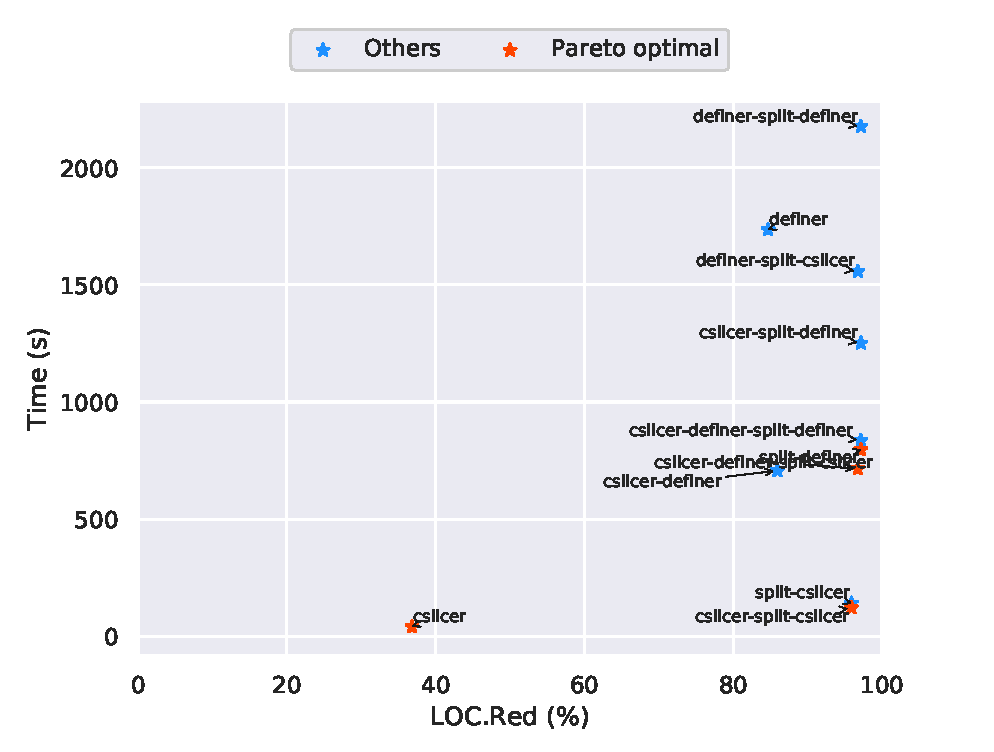
\includegraphics[scale=0.7]{plots/pareto/NET-527-pareto}
\caption{NET-527}
\end{figure}


%% Automatically generated by gen_all_configs_tables.py
\begin{table*}[t]
\begin{small}
\begin{center}
\caption{\TableCaptionSmallHistoryInfo}
\begin{tabular}{l|rr|rr}
\toprule
\TableHeadExampleId & \TableHeadNumOfFilesChanged & \TableHeadOrigHisLen & \TableHeadAvgNumOfChangedFilesPerCommit & \TableHeadAvgNumOfFeaturesPerCommit \\
\midrule
LANG-993 & \UseMacro{LANG993SplitHisLen} & \UseMacro{LANG993OrigHisLen} & \UseMacro{LANG993OrigAvgNumOfChangedFilesPerCommit} & \UseMacro{LANG993OrigAvgNumOfFeaturesPerCommit} \\
LANG-1006 & \UseMacro{LANG1006SplitHisLen} & \UseMacro{LANG1006OrigHisLen} & \UseMacro{LANG1006OrigAvgNumOfChangedFilesPerCommit} & \UseMacro{LANG1006OrigAvgNumOfFeaturesPerCommit} \\
IO-173 & \UseMacro{IO173SplitHisLen} & \UseMacro{IO173OrigHisLen} & \UseMacro{IO173OrigAvgNumOfChangedFilesPerCommit} & \UseMacro{IO173OrigAvgNumOfFeaturesPerCommit} \\
IO-275 & \UseMacro{IO275SplitHisLen} & \UseMacro{IO275OrigHisLen} & \UseMacro{IO275OrigAvgNumOfChangedFilesPerCommit} & \UseMacro{IO275OrigAvgNumOfFeaturesPerCommit} \\
IO-288 & \UseMacro{IO288SplitHisLen} & \UseMacro{IO288OrigHisLen} & \UseMacro{IO288OrigAvgNumOfChangedFilesPerCommit} & \UseMacro{IO288OrigAvgNumOfFeaturesPerCommit} \\
IO-290 & \UseMacro{IO290SplitHisLen} & \UseMacro{IO290OrigHisLen} & \UseMacro{IO290OrigAvgNumOfChangedFilesPerCommit} & \UseMacro{IO290OrigAvgNumOfFeaturesPerCommit} \\
IO-305 & \UseMacro{IO305SplitHisLen} & \UseMacro{IO305OrigHisLen} & \UseMacro{IO305OrigAvgNumOfChangedFilesPerCommit} & \UseMacro{IO305OrigAvgNumOfFeaturesPerCommit} \\
COMPRESS-327 & \UseMacro{COMPRESS327SplitHisLen} & \UseMacro{COMPRESS327OrigHisLen} & \UseMacro{COMPRESS327OrigAvgNumOfChangedFilesPerCommit} & \UseMacro{COMPRESS327OrigAvgNumOfFeaturesPerCommit} \\
COMPRESS-369 & \UseMacro{COMPRESS369SplitHisLen} & \UseMacro{COMPRESS369OrigHisLen} & \UseMacro{COMPRESS369OrigAvgNumOfChangedFilesPerCommit} & \UseMacro{COMPRESS369OrigAvgNumOfFeaturesPerCommit} \\
COMPRESS-373 & \UseMacro{COMPRESS373SplitHisLen} & \UseMacro{COMPRESS373OrigHisLen} & \UseMacro{COMPRESS373OrigAvgNumOfChangedFilesPerCommit} & \UseMacro{COMPRESS373OrigAvgNumOfFeaturesPerCommit} \\
COMPRESS-374 & \UseMacro{COMPRESS374SplitHisLen} & \UseMacro{COMPRESS374OrigHisLen} & \UseMacro{COMPRESS374OrigAvgNumOfChangedFilesPerCommit} & \UseMacro{COMPRESS374OrigAvgNumOfFeaturesPerCommit} \\
COMPRESS-375 & \UseMacro{COMPRESS375SplitHisLen} & \UseMacro{COMPRESS375OrigHisLen} & \UseMacro{COMPRESS375OrigAvgNumOfChangedFilesPerCommit} & \UseMacro{COMPRESS375OrigAvgNumOfFeaturesPerCommit} \\
CSV-159 & \UseMacro{CSV159SplitHisLen} & \UseMacro{CSV159OrigHisLen} & \UseMacro{CSV159OrigAvgNumOfChangedFilesPerCommit} & \UseMacro{CSV159OrigAvgNumOfFeaturesPerCommit} \\
CSV-175 & \UseMacro{CSV175SplitHisLen} & \UseMacro{CSV175OrigHisLen} & \UseMacro{CSV175OrigAvgNumOfChangedFilesPerCommit} & \UseMacro{CSV175OrigAvgNumOfFeaturesPerCommit} \\
CSV-180 & \UseMacro{CSV180SplitHisLen} & \UseMacro{CSV180OrigHisLen} & \UseMacro{CSV180OrigAvgNumOfChangedFilesPerCommit} & \UseMacro{CSV180OrigAvgNumOfFeaturesPerCommit} \\
NET-527 & \UseMacro{NET527SplitHisLen} & \UseMacro{NET527OrigHisLen} & \UseMacro{NET527OrigAvgNumOfChangedFilesPerCommit} & \UseMacro{NET527OrigAvgNumOfFeaturesPerCommit} \\
\bottomrule
\end{tabular}
\end{center}
\end{small}
\end{table*}

%% Automatically generated by gen_all_configs_tables.py
\begin{table*}[t]
\begin{small}
\begin{center}
\caption{\TableCaptionEndToEndTime}
\makebox[\linewidth][c]{\begin{tabular}{l|rrr|rr}
\toprule
\TableHeadExampleId & \TableHeadTimeWithoutCache & \TableHeadTimeWithPrefixCache & \TableHeadTimeWithSuffixCache & \TableHeadPrefixCacheSavingPercentage & \TableHeadSuffixCacheSavingPercentage \\
\midrule
IO-173 & \UseMacro{IO173NoOpEndToEndTime} & \UseMacro{IO173SharePrefixEndToEndTime} & \UseMacro{IO173ShareSuffixEndToEndTime} & \UseMacro{IO173SharePrefixSavingPercentage} & \UseMacro{IO173ShareSuffixSavingPercentage} \\
IO-275 & \UseMacro{IO275NoOpEndToEndTime} & \UseMacro{IO275SharePrefixEndToEndTime} & \UseMacro{IO275ShareSuffixEndToEndTime} & \UseMacro{IO275SharePrefixSavingPercentage} & \UseMacro{IO275ShareSuffixSavingPercentage} \\
IO-288 & \UseMacro{IO288NoOpEndToEndTime} & \UseMacro{IO288SharePrefixEndToEndTime} & \UseMacro{IO288ShareSuffixEndToEndTime} & \UseMacro{IO288SharePrefixSavingPercentage} & \UseMacro{IO288ShareSuffixSavingPercentage} \\
IO-290 & \UseMacro{IO290NoOpEndToEndTime} & \UseMacro{IO290SharePrefixEndToEndTime} & \UseMacro{IO290ShareSuffixEndToEndTime} & \UseMacro{IO290SharePrefixSavingPercentage} & \UseMacro{IO290ShareSuffixSavingPercentage} \\
IO-305 & \UseMacro{IO305NoOpEndToEndTime} & \UseMacro{IO305SharePrefixEndToEndTime} & \UseMacro{IO305ShareSuffixEndToEndTime} & \UseMacro{IO305SharePrefixSavingPercentage} & \UseMacro{IO305ShareSuffixSavingPercentage} \\
CSV-159 & \UseMacro{CSV159NoOpEndToEndTime} & \UseMacro{CSV159SharePrefixEndToEndTime} & \UseMacro{CSV159ShareSuffixEndToEndTime} & \UseMacro{CSV159SharePrefixSavingPercentage} & \UseMacro{CSV159ShareSuffixSavingPercentage} \\
CSV-175 & \UseMacro{CSV175NoOpEndToEndTime} & \UseMacro{CSV175SharePrefixEndToEndTime} & \UseMacro{CSV175ShareSuffixEndToEndTime} & \UseMacro{CSV175SharePrefixSavingPercentage} & \UseMacro{CSV175ShareSuffixSavingPercentage} \\
CSV-180 & \UseMacro{CSV180NoOpEndToEndTime} & \UseMacro{CSV180SharePrefixEndToEndTime} & \UseMacro{CSV180ShareSuffixEndToEndTime} & \UseMacro{CSV180SharePrefixSavingPercentage} & \UseMacro{CSV180ShareSuffixSavingPercentage} \\
NET-525 & \UseMacro{NET525NoOpEndToEndTime} & \UseMacro{NET525SharePrefixEndToEndTime} & \UseMacro{NET525ShareSuffixEndToEndTime} & \UseMacro{NET525SharePrefixSavingPercentage} & \UseMacro{NET525ShareSuffixSavingPercentage} \\
\midrule
Avg & \UseMacro{AvgNoOpEndToEndTime} & \UseMacro{AvgSharePrefixEndToEndTime} & \UseMacro{AvgShareSuffixEndToEndTime} & \UseMacro{AvgSharePrefixSavingPercentage} & \UseMacro{AvgShareSuffixSavingPercentage} \\
\bottomrule
\end{tabular}
}
\end{center}
\end{small}
\end{table*}


\end{document}
